% tm project ignores: !(/\.(?!htaccess)[^/]*|\.(tmproj|o|pyc|toc|aux|xyc|bbl|blg|lof|lot|out|synctex\.gz)|/Icon\r|/svn-commit(\.[2-9])?\.tmp)$

%   Modified   92-09-18      Add references to dissertation        D. Teale
%                            Add approval page to toc
%                            Add ref to Title Degree on approval page
%   Modified  2006-09-12     Added geometry package to set up UofC thesis margins
%                            Removed includeprompt option N. Mancell
%
% Modified  2012-04-15  T.Zhang
% 1, the ``fancy'' package is cancelled. The pagestyle is changed from ``myheadings''
%    and ``headings'' to ``plain'' to move the page number (footer) from top right to bottom centre.
% 2, The parameter  of using ``geometry'' package is changed from four different values
%     (top=1in, bottom=1.22in, left=1.40in, right=0.850in) to one single value:
%     1in (top=1in, bottom= 1in, left= 1in, right= 1in)
% 3, ``List of Figures'' is modified to ``List of Figures and Illustrations''
% 4, A new page ``List of Symbols, Abbreviations and Nomenclature'' is created.
%    Its page number is following ``List of Figures and Illustrations'' with Roman numerals.
%    A separate file ``symbols.tex'' is created for students to put content into the list.





\documentclass{ucalgthes1}
\usepackage[letterpaper,top=1in, bottom= 1in, left= 1in, right= 1in]{geometry}
%\usepackage{fancyhdr}
%\fancyhead{}
%\fancyfoot{}
%\renewcommand{\headrulewidth}{0pt}
%\fancyhead[RO,LE]{\thepage}
%Define other usepackages here

%!TEX root = /Users/gilesb/UofC/thesis/phd-thesis/phd-thesis.tex
\usepackage[T1]{fontenc}
\usepackage[utf8]{inputenc}
\usepackage{palatino,courier}
\usepackage[reqno]{amsmath}
\usepackage{amsthm}
\usepackage{amsfonts,amssymb}
\usepackage[mathscr]{euscript}
\usepackage[all]{xy}
\usepackage{stmaryrd}
\usepackage{graphicx}
\usepackage{array}
\usepackage{fancyvrb}
\usepackage{proof}
\usepackage{mchaskell}
\usepackage{float}
\usepackage{makeidx}
\usepackage{url}
\usepackage{varioref}
\usepackage{listings}

\usepackage{mylhs}
\usepackage{wrapfig}
\usepackage{subfig}
\usepackage{caption}
\usepackage{supertabular}

\usepackage{varioref}
\usepackage{xspace}
% \usepackage[colorlinks=true,citecolor=magenta]{hyperref} Causes issues!!!
\usepackage{hyperref}
%\usepackage{lqpl}
%\usepackage{prettyref}
%\usepackage{lucidabr}

\reversemarginpar

%\captionsetup{style=default,labelfont={bf}}
\def\figurename{Figure}
\def\tablename{Table}



\graphicspath{{./diagrams/}{.}}
%
%include lhs2TeX.fmt
%include lhs2TeX.sty
%format ^* = "\ltimes"
%format *^ = "\rtimes"
% captionskips do not seem to be defined in uc class
\makeatletter
%%\newlength\abovecaptionskip
%%\newlength\belowcaptionskip
\setlength\abovecaptionskip{10\p@}
\setlength\belowcaptionskip{0\p@}
\makeatother

%!TEX root = /Users/gilesb/UofC/thesis/phd-thesis/phd-thesis.tex
%\floatstyle{boxed}
%\newfloat{QuantumCircuit}{htp}{qci}[chapter]
%\floatname{QuantumCircuit}{Circuit}

%\setlength{\textheight}{8.5in}
%\setlength{\textwidth}{6.5in}
%\setlength{\oddsidemargin}{-.3in}
%\setlength{\evensidemargin}{-.3in}
% macros for processing of the literate files

% reference formats -
\labelformat{chapter}{chapter~#1}
\labelformat{section}{section~#1}
\labelformat{subsection}{sub-section~#1}
\labelformat{subsubsection}{sub-sub-section~#1}
\labelformat{equation}{equation~(#1)}
\labelformat{table}{table~#1}
\labelformat{figure}{figure~#1}


\DefineVerbatimEnvironment%
 {happycodefirst}{Verbatim}{gobble=2,numbers=left,firstnumber=1,fontsize=\footnotesize}
\DefineVerbatimEnvironment%
 {qplcodethesis}{Verbatim}{commandchars=\\\{\},numbers=left,firstnumber=1,fontsize=\footnotesize}
\DefineVerbatimEnvironment%
 {bnf}{Verbatim}{commandchars=\\\{\},fontfamily=courier,fontsize=\footnotesize}
\DefineVerbatimEnvironment%
 {happycodecont}{Verbatim}{gobble=2,numbers=left,firstnumber=last,fontsize=\footnotesize}
% import and redefinition of general macros
%!TEX root = /Users/gilesb/UofC/thesis/phd-thesis/phd-thesis.tex
\newcommand{\bproofenum}{\vspace{12pt} \hspace{-12pt} \renewcommand{\theenumi}{(\roman{enumi})}\renewcommand{\labelenumi}{\theenumi}\begin{enumerate}}
\newcommand{\eproofenum}{\end{enumerate}\renewcommand{\theenumi}{\arabic{enumi}}\renewcommand{\labelenumi}{\theenumi.}}
\newcommand{\bproofitemize}{ \vspace{12pt} \hspace{-12pt} \begin{itemize}}
\newcommand{\eproofitemize}{\end{itemize}}
\newcommand{\bproofdesc}{ \vspace{12pt} \hspace{-12pt} \begin{description}}
\newcommand{\eproofdesc}{\end{description}}
\newcommand{\bi}{\begin{itemize}}
\newcommand{\ei}{\end{itemize}}
\newcommand{\be}{\begin{enumerate}}
\newcommand{\ee}{\end{enumerate}}
\newcommand{\bd}{\begin{description}}
\newcommand{\ed}{\end{description}}
\newcommand{\itembf}[1]{\item{\textbf{#1}}}
\newcommand{\itemem}[1]{\item{\emph{#1}}}
\newcommand{\itemtt}[1]{\item{\texttt{#1}}}

\newcommand{\rone}{[\emph{\bfseries R.1}]\xspace}
\newcommand{\rtwo}{[\emph{\bfseries R.2}]\xspace}
\newcommand{\rthree}{[\emph{\bfseries R.3}]\xspace}
\newcommand{\rfour}{[\emph{\bfseries R.4}]\xspace}

\DeclareMathOperator*{\dom}{dom}
\DeclareMathOperator*{\rng}{range}
\newcommand{\nothing}{\phi}
\newcommand{\nin}{\ensuremath{\in\hspace{-0.8em}/\hspace{0.2em}}}

\newcommand{\BigO}[1]{\ensuremath{\mathscr{O}({#1})}}

\newcommand{\type}[1]{\ensuremath{\mathbf{{#1}}}\xspace}
\newcommand{\bit}{\type{bit}}
\newcommand{\qubit}{\type{qubit}}
\newcommand{\qubits}{\qubit{s}}
\newcommand{\bits}{\bit{s}}

\newcommand{\Qs}{\ensuremath{Q_{()}}\xspace}
\newcommand{\Bs}{\ensuremath{B_{()}}\xspace}

\newcommand{\mbf}{\ensuremath{\mathbf{f}}}
\newcommand{\mbg}{\ensuremath{\mathbf{g}}}
\newcommand{\mbh}{\ensuremath{\mathbf{h}}}

\newcommand{\restr}[1]{\overline{#1}}
\newcommand{\rst}[1]{\restr{#1}}
\newcommand{\cp}[1]{\amalg_{#1}}
\newcommand{\cpa}{\cp{0}}
\newcommand{\cpb}{\cp{1}}
\let\*\otimes
\let\+\oplus
\let\<\langle
\let\>\rangle
\newcommand{\uts}{\hspace{0.1pt}}


\newcommand{\spl}[2]{\ensuremath{\text{K}_{#1}(#2)}}
\newcommand{\capspl}{\ensuremath{\cap_{\text{K}}}\xspace}
\newcommand{\inv}[1]{\ensuremath{{#1}^{(-1)}}}
\newcommand{\dual}[1]{\ensuremath{{#1}^{*}}}
\newcommand{\dgr}[1]{\ensuremath{{#1}^{\dagger}}}

\newcommand{\uleft}[1]{\ensuremath{u_{#1}^l}}
\newcommand{\uright}[1]{\ensuremath{u_{#1}^r}}
\newcommand{\usl}{\uleft{\*}}
\newcommand{\usr}{\uright{\*}}
\newcommand{\upl}{\uleft{+}}
\newcommand{\upr}{\uright{+}}

\newcommand{\Xt}{\ensuremath{\widetilde{\X}}\xspace}


\newcommand{\hypXt}{\texorpdfstring{\Xt}{Xt}}
\newcommand{\hypX}{\texorpdfstring{\X}{X}}

\newcommand{\xtdmn}[2]{\ensuremath{{#1}_{|{#2}}}}


\newcommand{\xequiv}[1]{\ensuremath{\overset{\scriptscriptstyle #1}{\simeq}}}
\newcommand{\quest}[1]{\fbox{\fbox{\parbox{5in}{\footnotesize \textbf{ (Question): }#1}}}}
\newcommand{\note}[1]{\par\fbox{\fbox{\parbox{5in}{\footnotesize \textbf{(Internal Note): }#1}}}}
%\newcommand{\todo}[1]{\par\fbox{\fbox{\parbox{4in}{\footnotesize \textbf{2DO: }#1}}}}


\newcommand{\nm}{\ensuremath{n\times{}m}}
\newcommand{\mn}{\ensuremath{m\times{}n}}

\newcommand{\specialcat}[1]{\textsc{#1}\xspace}
\newcommand{\ltrcat}[1]{\ensuremath{\mathfrak{#1}}\xspace}
\newcommand{\ltrcatbb}[1]{\ensuremath{\mathbb{#1}}\xspace}
\newcommand{\B}{\ltrcatbb{B}}
\newcommand{\C}{\ltrcatbb{C}}
\newcommand{\D}{\ltrcatbb{D}}
\newcommand{\E}{\ltrcatbb{E}}
\newcommand{\Lat}{\ltrcatbb{L}}
\newcommand{\X}{\ltrcatbb{X}}

\newcommand{\Y}{\ltrcatbb{Y}}
\newcommand{\Z}{\ltrcatbb{Z}}

\newcommand{\complex}{\C}
\newcommand{\integers}{\Z}

\newcommand{\typecontext}{\ltrcatbb{T}}

\newcommand{\Hil}{\ensuremath{\mathcal{H}}\xspace}
\newcommand{\nat}{\ensuremath{\ltrcatbb{N}}\xspace}

\newcommand{\sets}{\specialcat{Sets}}
\newcommand{\rel}{\specialcat{Rel}}
\newcommand{\fdh}{\specialcat{FdHilb}}
\newcommand{\mon}{\specialcat{Mon}}
\newcommand{\ring}{\specialcat{Rng}}
\newcommand{\Par}{\specialcat{Par}}
\newcommand{\cring}{\specialcat{CRng}}
\newcommand{\cat}{\specialcat{Cat}}
\newcommand{\poset}{\specialcat{Poset}}
\newcommand{\preorder}{\specialcat{Preorder}}
\newcommand{\mcat}{\ensuremath{\mathcal{M}\text{\cat}}\xspace}

\newcommand{\Mstab}{\ensuremath{\mathcal{M}}\xspace}

\newcommand{\obj}[1]{\ensuremath{#1_{obj}}}
\newcommand{\bottom}[1]{\perp_{#1}}
\newcommand{\finpower}{\mathscr{P}_{fin}}

\newcommand{\category}[4]{%
\begin{description}%
\item{\textbf{Objects: }}{#1}%
\item{\textbf{Maps: }}{#2}%
\item{\textbf{Identity: }}{#3}%
\item{\textbf{Composition: }}{#4}%
 \end{description}%
%
}
\newcommand{\rcategory}[5]{%
\begin{description}%
\item{\textbf{Objects: }}{#1}%
\item{\textbf{Maps: }}{#2}%
\item{\textbf{Identity: }}{#3}%
\item{\textbf{Composition: }}{#4}%
\item{\textbf{Restriction: }}{#5}%
\end{description}%
%
}

\newcommand{\rcategoryequiv}[5]{%
\begin{description}%
\item{\textbf{Objects: }}{#1}%
\item{\textbf{Equivalence Classes of Maps: }}{#2}%
\item{\textbf{Identity: }}{#3}%
\item{\textbf{Composition: }}{#4}%
\item{\textbf{Restriction: }}{#5}%
\end{description}%
%
}

\newcommand{\pfcategory}[3]{%
\begin{description}%
\item{\textbf{Well-Defined: }}{#1}%
\item{\textbf{Identities: }}{#2}%
\item{\textbf{Associativity: }}{#3}%
\end{description}}


\newtheorem{theorem}{Theorem}[section]
\newtheorem{definition}[theorem]{Definition}
\newtheorem{proposition}[theorem]{Proposition}
\newtheorem{notation}[theorem]{Notation}
\newtheorem{notethm}[theorem]{Note}
\newtheorem{example}{Example}
\newtheorem{remark}{Remark}
\newtheorem{exercise}{Exercise}
\newtheorem{lemma}[theorem]{Lemma}
\newtheorem{corollary}[theorem]{Corollary}

%\theoremstyle{definition}
\newtheorem*{sltheorem}{Theorem}
\newtheorem*{sldefinition}{Definition}
\newtheorem*{slproposition}{Proposition}
\newtheorem*{slnotation}{Notation}
\newtheorem*{slexample}{Example}
\newtheorem*{slexercise}{Exercise}
\newtheorem*{sllemma}{Lemma}
% general math symbols
\newcommand{\union}{\ensuremath{\bigcup}}
\newcommand{\disjunion}{\ensuremath{\sqcup}}
\newcommand{\intersect}{\ensuremath{\bigcap}}
\newcommand{\logor}{\ensuremath{\lor}}
\newcommand{\logand}{\ensuremath{\land}}
\newcommand{\lognand}{\ensuremath{\barwedge}}
\newcommand{\natmap}{\ensuremath{\Rightarrow}}
\newcommand{\fctrmap}{\ensuremath{\to}}
\newcommand{\fnctrmap}{\fctrmap}
\newcommand{\fmap}{\ensuremath{\to}}
\newcommand{\produces}{\ensuremath{\to}}
\newcommand{\ladjoint}{\ensuremath{\dashv}}
\newcommand{\pproj}{\ensuremath{\preceq_p}}

\newcommand{\tr}[1]{\ensuremath{\text{tr}(#1)}}

\newcommand{\colvec}[1]{\ensuremath{
\begin{pmatrix}#1\end{pmatrix}}}

\newcommand{\tbtmatrix}[4]{\ensuremath{
\begin{pmatrix}
#1&#2\\
#3&#4
\end{pmatrix}
}}

\newcommand{\quadmatrix}[4]{\ensuremath{
\left(
\begin{array}{c|c}
#1&#2\\
\hline
#3&#4
\end{array}
\right)
}}


\newcommand{\nowiregate}[1]{*{\xy *+<.6em>{#1};p\save+LU;+RU **\dir{-}\restore\save+RU;+RD **\dir{-}\restore\save+RD;+LD **\dir{-}\restore\POS+LD;+LU **\dir{-}\endxy}}



\newcommand{\inflist}[1]{\ensuremath{\mathbb{IL}({#1})}}
\newcommand{\incsec}[1]{\subsection{#1}}
% end of redefinitions.
\newcommand{\incsubsec}[1]{\subsubsection{#1}}
\newcommand{\incsubsubsec}[1]{\paragraph{#1}}
\newcommand{\qplcode}[1]{\textbf{#1}}
\DefineVerbatimEnvironment%
{code}{Verbatim}{numbers=left,fontsize=\footnotesize,firstnumber=1}
\newcommand{\CodeResetNumbers}{\RecustomVerbatimEnvironment%
{code}{Verbatim}{numbers=left,fontsize=\footnotesize,firstnumber=1}}
\newcommand{\CodeContinueNumbers}{\RecustomVerbatimEnvironment%
{code}{Verbatim}{numbers=left,fontsize=\footnotesize,firstnumber=last}}
\renewcommand{\C}{\ensuremath{\mathbb{C}}}

%    Q-circuit version 2
%    Copyright (C) 2004  Steve Flammia & Bryan Eastin
%    Last modified on: 9/16/2011
%
%    This program is free software; you can redistribute it and/or modify
%    it under the terms of the GNU General Public License as published by
%    the Free Software Foundation; either version 2 of the License, or
%    (at your option) any later version.
%
%    This program is distributed in the hope that it will be useful,
%    but WITHOUT ANY WARRANTY; without even the implied warranty of
%    MERCHANTABILITY or FITNESS FOR A PARTICULAR PURPOSE.  See the
%    GNU General Public License for more details.
%
%    You should have received a copy of the GNU General Public License
%    along with this program; if not, write to the Free Software
%    Foundation, Inc., 59 Temple Place, Suite 330, Boston, MA  02111-1307  USA

% Thanks to the Xy-pic guys, Kristoffer H Rose, Ross Moore, and Daniel Müllner,
% for their help in making Qcircuit work with Xy-pic version 3.8.
% Thanks also to Dave Clader, Andrew Childs, Rafael Possignolo, Tyson Williams,
% Sergio Boixo, Cris Moore, Jonas Anderson, and Stephan Mertens for helping us test
% and/or develop the new version.

\usepackage{xy}
\xyoption{matrix}
\xyoption{frame}
\xyoption{arrow}
\xyoption{arc}

\usepackage{ifpdf}
\ifpdf
\else
\PackageWarningNoLine{Qcircuit}{Qcircuit is loading in Postscript mode.  The Xy-pic options ps and dvips will be loaded.  If you wish to use other Postscript drivers for Xy-pic, you must modify the code in Qcircuit.tex}
%    The following options load the drivers most commonly required to
%    get proper Postscript output from Xy-pic.  Should these fail to work,
%    try replacing the following two lines with some of the other options
%    given in the Xy-pic reference manual.
\xyoption{ps}
\xyoption{dvips}
\fi

% The following resets Xy-pic matrix alignment to the pre-3.8 default, as
% required by Qcircuit.
\entrymodifiers={!C\entrybox}

\newcommand{\bra}[1]{\ensuremath{\left\langle{#1}\right\vert}\xspace}
\newcommand{\ket}[1]{\ensuremath{\left\vert{#1}\right\rangle}\xspace}
    % Defines Dirac notation. %7/5/07 added extra braces so that the commands will work in subscripts.
\newcommand{\qw}[1][-1]{\ar @{-} [0,#1]}
    % Defines a wire that connects horizontally.  By default it connects to the object on the left of the current object.
    % WARNING: Wire commands must appear after the gate in any given entry.
\newcommand{\dqw}[1][-1]{\ar @{.} [0,#1]}
    % Defines a dotted wire that connects horizontally.  By default it connects to the object on the left of the current object.
    % WARNING: Wire commands must appear after the gate in any given entry.
\newcommand{\qwx}[1][-1]{\ar @{-} [#1,0]}
    % Defines a wire that connects vertically.  By default it connects to the object above the current object.
    % WARNING: Wire commands must appear after the gate in any given entry.
\newcommand{\cw}[1][-1]{\ar @{=} [0,#1]}
    % Defines a classical wire that connects horizontally.  By default it connects to the object on the left of the current object.
    % WARNING: Wire commands must appear after the gate in any given entry.
\newcommand{\cwx}[1][-1]{\ar @{=} [#1,0]}
    % Defines a classical wire that connects vertically.  By default it connects to the object above the current object.
    % WARNING: Wire commands must appear after the gate in any given entry.
\newcommand{\gate}[1]{*+<.6em>{#1} \POS ="i","i"+UR;"i"+UL **\dir{-};"i"+DL **\dir{-};"i"+DR **\dir{-};"i"+UR **\dir{-},"i" \qw}
    % Boxes the argument, making a gate.
\newcommand{\meter}{*=<1.8em,1.4em>{\xy ="j","j"-<.778em,.322em>;{"j"+<.778em,-.322em> \ellipse ur,_{}},"j"-<0em,.4em>;p+<.5em,.9em> **\dir{-},"j"+<2.2em,2.2em>*{},"j"-<2.2em,2.2em>*{} \endxy} \POS ="i","i"+UR;"i"+UL **\dir{-};"i"+DL **\dir{-};"i"+DR **\dir{-};"i"+UR **\dir{-},"i" \qw}
    % Inserts a measurement meter.
    % In case you're wondering, the constants .778em and .322em specify
    % one quarter of a circle with radius 1.1em.
    % The points added at + and - <2.2em,2.2em> are there to strech the
    % canvas, ensuring that the size is unaffected by erratic spacing issues
    % with the arc.
\newcommand{\measure}[1]{*+[F-:<.9em>]{#1} \qw}
    % Inserts a measurement bubble with user defined text.
\newcommand{\measuretab}[1]{*{\xy*+<.6em>{#1}="e";"e"+UL;"e"+UR **\dir{-};"e"+DR **\dir{-};"e"+DL **\dir{-};"e"+LC-<.5em,0em> **\dir{-};"e"+UL **\dir{-} \endxy} \qw}
    % Inserts a measurement tab with user defined text.
\newcommand{\measureD}[1]{*{\xy*+=<0em,.1em>{#1}="e";"e"+UR+<0em,.25em>;"e"+UL+<-.5em,.25em> **\dir{-};"e"+DL+<-.5em,-.25em> **\dir{-};"e"+DR+<0em,-.25em> **\dir{-};{"e"+UR+<0em,.25em>\ellipse^{}};"e"+C:,+(0,1)*{} \endxy} \qw}
    % Inserts a D-shaped measurement gate with user defined text.
\newcommand{\multimeasure}[2]{*+<1em,.9em>{\hphantom{#2}} \qw \POS[0,0].[#1,0];p !C *{#2},p \drop\frm<.9em>{-}}
    % Draws a multiple qubit measurement bubble starting at the current position and spanning #1 additional gates below.
    % #2 gives the label for the gate.
    % You must use an argument of the same width as #2 in \ghost for the wires to connect properly on the lower lines.
\newcommand{\multimeasureD}[2]{*+<1em,.9em>{\hphantom{#2}} \POS [0,0]="i",[0,0].[#1,0]="e",!C *{#2},"e"+UR-<.8em,0em>;"e"+UL **\dir{-};"e"+DL **\dir{-};"e"+DR+<-.8em,0em> **\dir{-};{"e"+DR+<0em,.8em>\ellipse^{}};"e"+UR+<0em,-.8em> **\dir{-};{"e"+UR-<.8em,0em>\ellipse^{}},"i" \qw}
    % Draws a multiple qubit D-shaped measurement gate starting at the current position and spanning #1 additional gates below.
    % #2 gives the label for the gate.
    % You must use an argument of the same width as #2 in \ghost for the wires to connect properly on the lower lines.
\newcommand{\control}{*!<0em,.025em>-=-<.2em>{\bullet}}
    % Inserts an unconnected control.
\newcommand{\controlo}{*+<.01em>{\xy -<.095em>*\xycircle<.19em>{} \endxy}}
    % Inserts a unconnected control-on-0.
\newcommand{\ctrl}[1]{\control \qwx[#1] \qw}
    % Inserts a control and connects it to the object #1 wires below.
\newcommand{\ctrlo}[1]{\controlo \qwx[#1] \qw}
    % Inserts a control-on-0 and connects it to the object #1 wires below.
\newcommand{\targ}{*+<.02em,.02em>{\xy ="i","i"-<.39em,0em>;"i"+<.39em,0em> **\dir{-}, "i"-<0em,.39em>;"i"+<0em,.39em> **\dir{-},"i"*\xycircle<.4em>{} \endxy} \qw}
    % Inserts a CNOT target.
\newcommand{\qswap}{*=<0em>{\times} \qw}
    % Inserts half a swap gate.
    % Must be connected to the other swap with \qwx.
\newcommand{\multigate}[2]{*+<1em,.9em>{\hphantom{#2}} \POS [0,0]="i",[0,0].[#1,0]="e",!C *{#2},"e"+UR;"e"+UL **\dir{-};"e"+DL **\dir{-};"e"+DR **\dir{-};"e"+UR **\dir{-},"i" \qw}
    % Draws a multiple qubit gate starting at the current position and spanning #1 additional gates below.
    % #2 gives the label for the gate.
    % You must use an argument of the same width as #2 in \ghost for the wires to connect properly on the lower lines.
\newcommand{\ghost}[1]{*+<1em,.9em>{\hphantom{#1}} \qw}
    % Leaves space for \multigate on wires other than the one on which \multigate appears.  Without this command wires will cross your gate.
    % #1 should match the second argument in the corresponding \multigate.
\newcommand{\push}[1]{*{#1}}
    % Inserts #1, overriding the default that causes entries to have zero size.  This command takes the place of a gate.
    % Like a gate, it must precede any wire commands.
    % \push is useful for forcing columns apart.
    % NOTE: It might be useful to know that a gate is about 1.3 times the height of its contents.  I.e. \gate{M} is 1.3em tall.
    % WARNING: \push must appear before any wire commands and may not appear in an entry with a gate or label.
\newcommand{\gategroup}[6]{\POS"#1,#2"."#3,#2"."#1,#4"."#3,#4"!C*+<#5>\frm{#6}}
    % Constructs a box or bracket enclosing the square block spanning rows #1-#3 and columns=#2-#4.
    % The block is given a margin #5/2, so #5 should be a valid length.
    % #6 can take the following arguments -- or . or _\} or ^\} or \{ or \} or _) or ^) or ( or ) where the first two options yield dashed and
    % dotted boxes respectively, and the last eight options yield bottom, top, left, and right braces of the curly or normal variety.  See the Xy-pic reference manual for more options.
    % \gategroup can appear at the end of any gate entry, but it's good form to pick either the last entry or one of the corner gates.
    % BUG: \gategroup uses the four corner gates to determine the size of the bounding box.  Other gates may stick out of that box.  See \prop.

\newcommand{\rstick}[1]{*!L!<-.5em,0em>=<0em>{#1}}
    % Centers the left side of #1 in the cell.  Intended for lining up wire labels.  Note that non-gates have default size zero.
\newcommand{\lstick}[1]{*!R!<.5em,0em>=<0em>{#1}}
    % Centers the right side of #1 in the cell.  Intended for lining up wire labels.  Note that non-gates have default size zero.
\newcommand{\ustick}[1]{*!D!<0em,-.5em>=<0em>{#1}}
    % Centers the bottom of #1 in the cell.  Intended for lining up wire labels.  Note that non-gates have default size zero.
\newcommand{\dstick}[1]{*!U!<0em,.5em>=<0em>{#1}}
    % Centers the top of #1 in the cell.  Intended for lining up wire labels.  Note that non-gates have default size zero.
\newcommand{\Qcircuit}{\xymatrix @*=<0em>}
\newcommand{\Qcircuitnocompile}{\xymatrixnocompile @*=<0em>}
    % Defines \Qcircuit as an \xymatrix with entries of default size 0em.
\newcommand{\link}[2]{\ar @{-} [#1,#2]}
    % Draws a wire or connecting line to the element #1 rows down and #2 columns forward.
\newcommand{\pureghost}[1]{*+<1em,.9em>{\hphantom{#1}}}
    % Same as \ghost except it omits the wire leading to the left.
 % for quantum circuits

\newcommand{\marginnote}[1]{\marginpar{\tiny #1}}



\lstdefinestyle{hskl}{language=Haskell,
%  basicstyle=\small, % swap this and the following line for prop. font
  basicstyle=\small,
%  keywordstyle=\underbar, % these look ugly
  identifierstyle=\itshape,
  commentstyle=\ttfamily,
%  commentstyle=\underbar
  flexiblecolumns=false,
  basewidth={0.5em,0.45em},
  morekeywords={Map},
  % The following replace compound charcters like ->
  % Something is missing - someone kindly sent me an email which
  % I've lost - but it's obvious how to add more.
  literate={-}{{$-$}}1 {+}{{$+$}}1 {/}{{$/$}}1
     {*}{{$\times$}}1 {=}{{$=$}}1
     {\%}{{$\%$}}1 {=}{{$=$}}1
           {>}{{$>$}}1 {<}{{$<$}}1
           {>>}{{$\gg$}}2 {<<}{{$\ll$}}2
           {=>}{{$\Rightarrow$}}2 {>=}{{$\geq$}}2 {<-}{{$\leftarrow$}}2
           {<=}{{$\leq$}}2
           {<==}{{$\Longleftarrow$}}3
           {=/=}{{$\neq$}}3
}
\lstdefinestyle{origlinqpl}{language=lqpl,basicstyle=\footnotesize\ttfamily,%
  numbers=left,%
        numberstyle=\tiny,%
        numbersep=6pt }
\lstdefinestyle{linqpl}{language=lqpl,basicstyle=\footnotesize,%
  numbers=left,%
        numberstyle=\tiny,%
        numbersep=6pt,%
  escapechar=`,%
  literate={-}{{$-$}}1 {+}{{$+$}}1 {/}{{$/$}}1%
     {*}{{$\times$}}1 {=}{{$=$}}1%
     {\%}{{$\%$}}1 {=}{{$=$}}1%
           {>}{{$>$}}1 {<}{{$<$}}1%
           {>>}{{$\gg$}}2 {<<}{{$\ll$}}2%
           {=>}{{$\Rightarrow$}}2 {>=}{{$\geq$}}2%
           {=<}{{$\leq$}}2%
           {<=}{{$\Leftarrow$}}3%
           {=/=}{{$\neq$}}3 }
\lstdefinestyle{inlinqpl}{language=lqpl,basicstyle=\footnotesize\ttfamily,%
  escapechar=`}

\newcommand{\lbl}{{\cdptr}}
\newcommand{\cd}{\ensuremath{\mathcal{C}}}
\newcommand{\lblcd}{{\cd}}
%\newcommand{\lblcd}{\ensuremath{@\lbl}}
\newcommand{\cdptr}{\ensuremath{\triangleright\cd}}
%\newcommand{\ 2 do}[1]{\begin{quote}2 do: \textbf{#1}\end{quote}}
\newcommand{\lqpl}{L-QPL}
\newcommand{\linearqpl}{Linear QPL}

\newcommand{\inlqpl}[1]{\protect{\lstinline[style=inlinqpl]!#1!}}
\newcommand{\inlhskl}[1]{\lstinline[style=hskl]!#1!}


\newcommand{\Had}{\text{Hadamard}}
\newcommand{\nottr}{\text{Not}}
\newcommand{\Cnot}{controlled{-}\nottr}

\newcommand{\stacknode}[1]{\ensuremath{\mathrm{\texttt{#1}}}}
\newcommand{\Int}{\stacknode{Int}}
\newcommand{\Datatype}{\stacknode{datatype}}
\newcommand{\Bool}{\stacknode{Bool}}

\newcommand{\vc}[1]{\ensuremath{\mathbold{#1}}}
\newcommand{\syntacticset}[1]{\ensuremath{\mathbold{#1}}}

\newcommand{\n}{\syntacticset{N}}
\newcommand{\T}{\syntacticset{T}}
\newcommand{\Q}{\syntacticset{Q}}
\newcommand{\R}{\syntacticset{R}}
\newcommand{\Data}{\syntacticset{Data}}
\newcommand{\Qloc}{\syntacticset{Qloc}}
\newcommand{\Cloc}{\syntacticset{Cloc}}
\newcommand{\Loc}{\syntacticset{Loc}}
\newcommand{\Aexp}{\syntacticset{Aexp}}
\newcommand{\Bexp}{\syntacticset{Bexp}}
\newcommand{\Cexp}{\syntacticset{Cexp}}
\newcommand{\Stm}{\syntacticset{Stm}}
\newcommand{\eval}[3]{\ensuremath{\langle{#1},{#2}\rangle\to{#3}}}
\newcommand{\true}{\ensuremath{\mathbold{true}}}
\newcommand{\false}{\ensuremath{\mathbold{false}}}


\newcommand{\qcons}[1]{\texttt{#1}}
\newcommand{\qtype}[1]{\texttt{\bf{#1}}}
\newcommand{\bms}{\specialcat{Bqsm}}
\newcommand{\lbms}{\specialcat{lBqsm}}
\newcommand{\cms}{\specialcat{Cqsm}}
\newcommand{\ms}{\specialcat{QSM}}

\newcommand{\qsp}{\ensuremath{\to}}

\newcommand{\qsnodeij}[4]{\ensuremath{#1\{{#2}\qsp {#3}\}^{#4}}}

\newcommand{\qsbit}[4]{\ensuremath{#1\{0\qsp {#2};1\qsp {#3}\}^{#4}}}



\newcommand{\qsqubit}[6]{\ensuremath{#1\{00\qsp {#2};01\qsp {#3};10\qsp {#4};11\qsp {#5}\}^{#6}}}

\newcommand{\qsbitUp}[4]{\ensuremath{#1\left\{\begin{array}{l}%
                  0\qsp {#2}\\%
                        1\qsp {#3}%
                        \end{array}%
               \right\}^{#4}}}


\newcommand{\qsqubitUp}[6]{\ensuremath{#1\left\{\begin{array}{ll}%
                  00\qsp {#2};&01\qsp {#3}\\%
                        10\qsp {#4};&11\qsp {#5}%
                        \end{array}%
               \right\}^{#6}}}
\newcommand{\qsqubitAllUp}[6]{\ensuremath{#1\left\{\begin{array}{l}%
                  00\qsp {#2}\\%
                        01\qsp {#3}\\%
                        10\qsp {#4}\\%
                        11\qsp {#5}%
                        \end{array}%
               \right\}^{#6}}}

\newcommand{\eentail}{\ensuremath{\Vdash\!\!\dashv}}
\newcommand{\ientail}{\ensuremath{\Vdash}}
\newcommand{\qentail}{\ensuremath{\vdash}}
\newcommand{\qcontext}{\ensuremath{\, |\, }}
\newcommand{\qcontrolled}[2]{\ensuremath{{#1}\Leftarrow{#2}}}
\newcommand{\qvec}[1]{\ensuremath{\widetilde{#1}}}
\newcommand{\qop}[2]{\ensuremath{{#1}\cdot{#2}}}
\newcommand{\qopseq}[2]{\ensuremath{{#1};{#2}}}

\newcommand{\qresultsind}[3]{\ensuremath{{#2}\overset{#1}{\leadsto}{#3}}}
\newcommand{\qresultsin}[2]{\qresultsind{}{#1}{#2}}
\newcommand{\qresultsindUp}[3]{\ensuremath{\begin{array}{l}%
             {#2}\overset{#1}{\leadsto}\\%
  \qquad{#3}}%
          \end{array}}
\newcommand{\qresultsinUp}[2]{\qresultsindUp{}{#1}{#2}}
\newcommand{\stackthree}[3]{\ensuremath{\begin{array}{l}{#1}\\{#2}\\{#3}\end{array}}}
\newcommand{\stackthreec}[3]{\ensuremath{\begin{array}{c}{#1}\\{#2}\\{#3}\end{array}}}
\newcommand{\stacktwo}[2]{\ensuremath{\begin{array}{l}{#1}\\{#2}\end{array}}}
\newcommand{\stacktwoc}[2]{\ensuremath{\begin{array}{c}{#1}\\{#2}\end{array}}}
\newcommand{\qmeasnob}[3]{{\begin{singlespace}\stackthree{\text{meas }{#1}:}{\quad \ket{0}=>#2}{\quad \ket{1}=>#3}\end{singlespace}}}
\newcommand{\qmeas}[3]{{\begin{singlespace}\left\{\stackthree{\text{meas }{#1}:}{\ \ket{0}=>#2}{\ \ket{1}=>#3}\right\}\end{singlespace}}}
\newcommand{\qcompose}[2]{\ensuremath{{#1};{#2}}}
\newcommand{\qtensor}[2]{\ensuremath{{#1};;{#2}}}
\newcommand{\qins}{\ensuremath{\mathscr{I}}}
\newcommand{\qmod}{\ensuremath{\mathscr{M}}}
\newcommand{\qcase}[4]{{\begin{singlespace}\left\{\stacktwo{\text{case }{#1}:}{\{{\ {#2}=>{#3}}\}_{#4}}\right\}\end{singlespace}}}
\newcommand{\quse}[2]{{\left\{\text{use }{#1}:\ \{{#2}\}\right\}}}
\newcommand{\tcls}{\ensuremath{\tau_C}}
\newcommand{\semins}[1]{\texttt{#1}}
\newcommand{\qifelse}[6]{{\begin{singlespace}\left\{\stackthree{\text{if }{#1}=>{#2}}{{\{\ {#3}=>{#4}}\}_{#5}}{\text{else }=>{#6}}\right\}\end{singlespace}}}


\newcommand{\qsmins}[1]{\texttt{#1}}

\newcommand{\qsminsparm}[1]{\ensuremath{#1}}
\newcommand{\qsminswithp}[2]{\texttt{#1}\qsminsparm{\ #2}}
\newcommand{\dmpelemqc}{\text{\texttt{Qc}}}
\newcommand{\qsmbool}[1]{\text{\texttt{#1}}}
\newcommand{\qsmfalse}{\qsmbool{False}}
\newcommand{\qsmtrue}{\qsmbool{True}}
\newcommand{\qstackMod}[1]{\texttt{#1}}

\newcommand{\terminalio}[1]{\texttt{#1}}


\newcommand{\interpsem}[1]{\ensuremath{\left\llbracket {#1} \right\rrbracket}}

\newcommand{\Inflist}{\text{Inflist}}

\newcommand{\trspace}{\ensuremath{\qquad\qquad\qquad\qquad\qquad}}
\newcommand{\trbigspace}{\ensuremath{\qquad\qquad\qquad\qquad\qquad\qquad\qquad}}

\newcommand{\trspacefour}{\ensuremath{\qquad\qquad\qquad\qquad}}
\newcommand{\trspacethree}{\ensuremath{\qquad\qquad\qquad}}
\newcommand{\trspacetwo}{\ensuremath{\qquad\qquad}}

\newcommand{\ilsep}{\ensuremath{\blacktriangleright}}

\newcommand{\lqplmodifier}[1]{\text{\texttt{#1}}}
\newcommand{\IdOnly}{\lqplmodifier{IdOnly}}
\newcommand{\Left}{\lqplmodifier{Left}}
\newcommand{\Right}{\lqplmodifier{Right}}
\title{An investigation of the underpinnings of quantum and reversible computing \\
\bigskip subtitle }
%
%            Insert the correct information between the {}
%
\author{Brett Gordon Giles}
\thesisyear{2013}
\thesis{dissertation}    % the word dissertation can be inserted between {}
\newcommand{\thesistitle}{An investigation of the underpinnings of quantum and reversible computing}
\monthname{August}
\dept{COMPUTER SCIENCE}
\degree{DOCTOR OF PHILOSOPHY}
%
%                    End of supplied information
%
\begin{document}
\makethesistitle
\pagenumbering{roman}     % resets page counter to one
\setcounter{page}{1}
%\chapter*{UNIVERSITY OF CALGARY \\ FACULTY OF GRADUATE STUDIES}
%\thispagestyle{empty}
%The undersigned certify that they have read, and recommend
%to the Faculty of Graduate Studies for acceptance, a \Thesis\ entitled
%``\thesistitle'' submitted by \Author\
%in partial fulfillment of the requirements for the degree of
%\Degree.\\

%
%                 Substitute  List of Examiners
%
%\begin{signing}{Department of Academic Computing}
%\signline
%Chairman, Dr.~John D.~Doe \\
%Department of Academic Computing \\
%Services  \\
%\signline
%Chairman, Dr.~John D.~Doe \\
%Department of Academic Computing \\
%Services  \\
%\signline
%Chairman, Dr.~John D.~Doe \\
%Department of Academic Computing \\
%Services  \\
%\signline
%Chairman, Dr.~John D.~Doe \\
%Department of Academic Computing \\
%Services  \\
%\newsigncolumn         use this command to start a new column if necessary
%\newsigncolumn
%\signline
%Chairman, Dr.~John D.~Doe \\
%Department of Academic Computing \\
%Services  \\
%\signline
%Dr.~Jane Smith \\
%Department of Academic Computing  \\

%\signline
%Dr.~A.~B.~Brown \\
%Department of Academic Computing  \\
%\end{signing}
%
\newpage
\phantomsection
\altchapter{\bf{Abstract}}

\newpage
\phantomsection
\altchapter{\bf{Acknowledgements}}


\begin{singlespace}
\newpage
\phantomsection
\tableofcontents
\pagestyle{plain}
\newpage
\phantomsection
\listoftables
\pagestyle{plain}
\newpage
\phantomsection
\listoffigures
\pagestyle{plain}
\clearpage
\clearpage          % otherwise tables will be numbered wrong
\end{singlespace}
\newpage
\phantomsection
\chapter*{\bf{List of Symbols, Abbreviations and Nomenclature}\hfill} \addcontentsline{toc}{chapter}{List of Symbols}
\listofsymbols
%\pagestyle{plain}
%\clearpage


\pagenumbering{arabic}
%!TEX root = /Users/gilesb/UofC/thesis/phd-thesis/phd-thesis.tex

\chapter{Category theory}\label{chap:category_theory}
\section{Categories} % (fold)
\label{sec:categories}

A category as a mathematical object can be defined in a variety of equivalent ways. As much of our
work will involve the exploration of partial and reversible maps, their domains and ranges, we
choose a definition that highlights the algebraic nature of these. Note that ranges are normally
referred to as codomains in category theory and we will use the codomain terminology in this
section.

\begin{definition}\label{def:category}
  A \emph{category} $\A$ is a collection of maps together with two functions, $D$ and $C$, from
  $\A$ to $\A$ and a partial associative composition of maps (written by juxtaposing maps), such
  that:
  \begin{itemize}
    \item[\catone] $D(f) f$ is defined and equals $f$,
    \item[\cattwo] $f C(f)$ is defined and equals $f$,
    \item[\catthree] $f g$ is defined iff $C(f) = D(g)$ and $D(f g) = D(f)$ and $C(f g) = C(g)$,
    \item[\catfour] $(f g) h = f (g h)$ whenever either side is defined,
    \item[\catfive] $D(C(x)) = C(X)$, $C(D(x)) = D(x)$ and $C,D$ are both idempotent.
  \end{itemize}
\end{definition}

A more familiar defintion, often used in introducing categories, is given next.

\begin{definition}\label{def:category_alt}
  A \emph{category} $\A$ is a directed graph consisting of objects $A_o$ and maps $A_m$. Each $f\in
  A_m$ has two associated objects in $A_o$, called the domain and codomain. When $f$ has domain $X$
  and codomain $Y$ we will write $f:X \to Y$. For $f, g \in A_m$, if $f:X\to Y$ and $g:Y \to Z$,
  there is a map called the \emph{composite} of $f$ and $g$, written $fg$ such that $fg:X \to Z$.
  For any $W \in A_o$ there is an \emph{identity} map $1_W:W \to W$. Additionally, these two axioms
  must hold:
  \begin{itemize}
    \item[\axiom{C'}{1}] for $f:X \to Y$, $1_X f = f = f 1_Y$,
    \item[\axiom{C'}{2}] given $f:X \to Y,\ g:Y \to Z$ and $h: Z\to W$, then $f (g h) = (f g) h$.
  \end{itemize}
  
\end{definition}

\begin{lemma}\label{lem:category_is_category_alt}
  A category as defined in Definition~\ref{def:category} is equivalent to a category as defined
  in Definition~\ref{def:category_alt} and vice versa.  
\end{lemma}
\begin{proof}
  Assume $\A$ is as in Definition~\ref{def:category}. Then set $A_o$ to the collection of all
  $D(f)$ and $C(f)$. Set $A_m$ to all the maps in $\A$. The domain of any map $f \in A_m$ is $D(f)$
  and the codomain is $C(f)$. By \catthree, for $f:X\to Y$ and $g:Y \to Z$ the composite $fg$ is
  defined. The identity map of the object $D(f)$ is the map $D(f)$ and the identity map of the
  object $C(f)$ is $C(f)$. By \catfive, we see \axiom{C'}{1} is satisfied. By \catfour, we see
  \axiom{C'}{2} is satisfied. Therefore, $\A$ satisfies Definition~\ref{def:category_alt}.
  
  Conversely, assume $\Z$ is as in Definition~\ref{def:category_alt}. Then, we already have the
  collection of maps, $Z_m$. For each $f : A \to B \in Z_m$, set $D(f) = 1_A$ and $C(f) = 1_B$. By
  the definition of the identity maps and \axiom{C'}{1}, we see \catone, \cattwo and \catfive are
  all satisfied. From the compostion requirements on $\Z$ and \axiom{C'}{2}, it follows that
  \catfour is satisfied. For \catthree, assume $f g$ is defined. Then for some $A,B,C \in Z_o$,
  $f:A \to B$ and $g:B \to C$. This gives us $1_B = C(f) = D(g)$, $1_A = D(f g) = D_f$ and $1_B =
  C(f g) = C(g)$. Next, assume we have $C(f) = D(g)$, $D(f g) = D(f)$ and $C(f g) = C(g)$. This
  tells us the codomain of $f$ is some object $B$ which is also the domain of $g$, hence we may
  form the composition $f g$ which will have domain $A$, the domain of $f$ and codomain $C$, the
  codomain of $g.$
\end{proof}

\subsection{Enrichement of categories} % (fold)
\label{sub:enrichement_of_categories}
\begin{definition}\label{def:hom-collection}
  If $\X$ is a category, then $\X(A,B)$ is called a \emph{hom-collection} of $\X$ and consists
  of all arrows $f$ with $D(f) = A$ and $C(f) = B$. 
\end{definition}

In the case where the hom-objects of a category $\X$ are all sets, we call them hom-sets. Additionally,
we say $\X$ is \emph{enriched} in \sets. We may extend this to any mathematical structure, e.g., 
enriched in partial orders, enriched in groups, etc..


Specific types of enrichment may force a specific structure on a category. For example, if $\X$ is
enriched in sets of cardinality of 0 or 1, then $\X$ must be a preorder. 
\subsection{Examples of categories} % (fold)
\label{sub:examples_of_categories}
In this section, we will offer a few examples of categories. As Definition~\ref{def:category_alt} 
tends to be a more succinct way to present the data of a category, this section will given the
examples in terms of objects and maps rather than the ``object-free'' definition.

% subsubsection categories_based_on_sets (end)

\subsubsection{Categories based on \protect{\sets}} % (fold)
\label{ssub:categories_based_on_sets}
There are three primary categories of interest to us where the objects are the collection of sets.
The first is \sets, where the maps are given by all set functions. The second is \Par, where the maps
are all partial maps. In each case, the standard definition of functions suffices to ensure indenties,
compositions and associativity are all satisfied. Domain and codomain are given by the domain and range
respectively.  

A third example, often of interest in quantum programming language semantics is \rel:
\category{Sets}{Relations: $R:X \to Y$}{$1_X = \{(x,x) | x \in X\}$}{$RS = \{(x,z) | 
\exists y, (x,y) \in R$ and $(y,z)\in S\}$}

Note that \rel is enriched in posets, via set inclusion. \Par can be viewed as a subcategory of
\rel, with the same objects, but only allowing maps which are functions, i.e., if $(x,y), (x,y')
\in R$, then $y = y'$. \Par is also enriched in posets, via the same inclusion ordering as in \rel.

\subsubsection{Matrix categories} % (fold)
\label{ssub:matrix_categories}
Given a rig $R$ (i.e., a ring minus negatives, e.g., the positive rationals), one may form the category
\specialcat{Mat}($R$).
\category{\nat}{$[r_{ij}]: n \to m$ where $[r_{ij}]$ is an $n \times m$ matrix over $R$}{
$I_n$}{Matrix multiplication}
% subsubsection matrix_categories (end)

\subsubsection{Functors and natural transformations} % (fold)
\label{ssub:functors_and_natural_transformations}

\begin{definition}\label{def:functor}
  A map $F:\X \to \Y$ between categories is called a \emph{functor}, provided it satisfies the following:
  \begin{itemize}
    \item[\axiom{F}{1}] $F(D(f)) = D(F(f))$ and $F(C(f)) = C(F(f))$;
    \item[\axiom{F}{2}] $F(f g) = F(f)F(g)$;
  \end{itemize}
\end{definition}

\begin{lemma}\label{lem:cat_is_a_category}
  The collection of categories and functors form the category \cat.
\end{lemma}
\begin{proof}
  \category{Categories.}{Functors.}{The identity functor which takes a map to the same map.}{
  $FG(x) = F(G(x))$ which is clearly associative.}
\end{proof}

\begin{definition}\label{def:natural_transformation}
  Given functors $F,G:\X \to \Y$, a \emph{natural transformation} $\alpha:F \natto G$ is a collection
  of maps in $\Y$, $\alpha_X : F(X) \to G(X)$, indexed by the objects of $\X$ such that for all
  $f:X_1 \to X_2$ in $\X$ the following diagram in $\Y$ commutes:
  \[\xymatrix @R+10pt @C+10pt{
      F(X_1) \ar[r]^{F(f)} \ar[d]_{\alpha_{X_1}} & F(X_2) \ar[d]^{\alpha_{X_2}}\\
      G(X_1) \ar[r]_{G(f)} &  G(X_2)
    }
  \]
\end{definition}
% subsubsection functors_and_natural_transformations (end)

% subsection examples_of_categories (end)
% subsection enrichement_of_categories (end)

% section categories (end)
\section{Restriction categories} % (fold)
\label{sec:restriction_categories}


Restriction categories were introduced in
 \cite{cockett2002:restcategories1} as a convenient axiomatization of partial maps.
\begin{definition}
  A \emph{restriction category} is a category \X\ together with a \emph{restriction operator} on
  maps:
  \[
    \infer{\restr{f}:A\to A}{f:A \to B}
  \]
  where $f$ is an map of \X\ and $A,B$ are objects of \X, such that the
  following four \emph{restriction identities} hold, whenever the
  compositions\footnote{Note that composition is
  written in diagrammatic order throughout this paper.} are defined.
  \begin{align*}
    &\rone\ \restr{f} f = f & &
    \rtwo\ \restr{g}  \restr{f} = \restr{f}  \restr{g}\\
    &\rthree\ \restr{\restr{f}  g} = \restr{f}   \restr{g} & &
    \rfour\  f \restr{g} = \restr{f g} f
  \end{align*}
\end{definition}

\begin{definition}
  A \emph{restriction functor} is a functor which preserves the restriction. That is,
  given a functor $F: \X \to \Y$ with \X\  and \Y\ restriction categories,
  $F$ is a restriction functor if:
  \[ 
    F(\restr{f}) = \restr{F(f)}.
  \]
\end{definition}

Any map such that $r=\restr{r}$ is an idempotent, as $\rst{r}\rst{r} = \rst{\rst{r} r} = \rst{r}$,
and is called a \emph{restriction idempotent}. All maps $\restr{f}$ are restriction idempotents as
$\rst{f}=\rst{\rst{f}}$. Below, we record some basic facts for restriction categories
shown in \cite{cockett2002:restcategories1} pp 4-5:
\begin{lemma}\label{lem:identities_involving_restriction}
  In a restriction category \X,
  \begin{multicols}{2}
    \begin{enumerate}[{(}i{)}]
      \item{}$\rst{f}$ is idempotent;
      \item{} $\rst{f g} = \rst{f g} \, \rst{f}$;\label{lemsub:restriction_identities_two}
      \item{} $\rst{f g} = \rst{f \rst{g}}$ ;
      \item{} $\rst{\rst{f}} = \rst{f}$;
      \item{} $\rst{f}\,\rst{g} = \rst{\rst{f}\,\rst{g}}$;
      \item{} $f$ monic implies $\rst{f} = 1$;
      \item{} $f = \rst{g} f \implies \rst{g}\,\rst{f} = \rst{f}$.
      \\
    \end{enumerate}
  \end{multicols}
\end{lemma}

A map $f:A\to B$ in a restriction category is said to be \emph{total} when
$\rst{f} = 1_A$. The total maps in a restriction category form a subcategory
$Total(\X) \subseteq \X$.

An example of a restriction category is \Par, the category with objects sets and arrows the 
partial functions between sets. In \Par, the restriction of $f:A\to B$ is:
\[
  \rst{f}(x) =
  \begin{cases}
    x&\text{if $f(x)$ is defined,}\\
    \uparrow&\text{if }f(x)\text{ is }\uparrow.
  \end{cases}
\]
(The symbol $\uparrow$ means that the function is undefined at that element). In \Par, the
total maps correspond precisely to the functions that are defined on all elements of the domain.


\subsection{Enrichment and meets} % (fold)
\label{sub:enrichment_and_meets}


In any restriction category, there is a partialorder on each hom-set, given by $f \le g$ iff
$\restr{f} g = f$, where $f,g:A\to B$.

\begin{lemma}\label{lem:restriction_cats_are_partial_order_enriched}
  In a restriction category \X:
  \begin{enumerate}[{(}i{)}]
    \item  $\le$ as defined  above is a partial order on each hom-set;
    \item $f \le g \implies \restr{f} \le \restr{g}$;
    \item $f \le g \implies h f \le h g$;
    \item $f \le g \implies f h \le g h$;
    \item $f \le 1 \iff f = \restr{f}$.
  \end{enumerate}
\end{lemma}
\begin{proof}
  \prepprooflist
  \begin{enumerate}[{(}i{)}]
    \item With $f,g,h$ parallel maps in \X, each of the requirements for a partial order is 
      shown below:
      \begin{description}
        \itembf{Reflexivity:} $\restr{f} f = f$ and therefore, $ f \le f$.
        \itembf{Anti-Symmetry:} Given $\restr{f}g = f$ and $\restr{g}f = g$, it follows:
          \[
            f = \restr{f} f = \restr{\restr{f} g} f = \restr{f}\, \restr{g} f
            = \restr{g}\restr{f} f =  \restr{g} f = g.
          \]
        \itembf{Transitivity:} Given $f \le g$ and $g\le h$,
          \[
            \restr{f} h = \restr{\restr{f} g} h = \restr{f}\, \restr{g} h = \restr{f} g = f
          \]
          showing that $f \le h$.
      \end{description}
    \item The premise is that $\restr{f} g = f$. From this,
      $ \restr{f}\, \restr{g} = \restr{\restr{f} g} = \restr{f}$, showing
      $\restr{f} \le \restr{g}$.
    \item $\restr{h f} hg = h \restr{f} g = h f$ and therefore $h f \le hg$.
    \item $\restr{f} g = f$, this shows  $\restr{f h} g h = \restr{\restr{f} g h} g h
      = \restr{f}\, \restr{g h} g h = \restr{f} g h = f h$ and therefore $f h \le g h$.
    \item As $f \le 1$ means precisely $\restr{f}1 = f$.
  \end{enumerate}
\end{proof}

Lemma \vref{lem:restriction_cats_are_partial_order_enriched} shows that restriction 
categories are enriched in partial orders.

\begin{definition}
  A restriction category has \emph{meets} if there is an operation $\cap$ on parallel maps:
  \[
    \infer{A\xrightarrow{f\cap g} B}
      {A\overset{f}{\underset{g}{\rightrightarrows}}B}
  \]
  such that $f\cap g \le f, f\cap g \le g, f\cap f = f, h (f\cap g) = h f \cap hg$.
\end{definition}

Meets were introduced in \cite{cockett-guo-hofstra-2012:range2}.
The following are basic results on meets:

\begin{lemma}
  \label{lem:properties_of_meets_in_restriction_categories}
  In a restriction category \X with meets, where $f, g, h$ are maps in
  \X, the following are true:
  \begin{enumerate}[{(}i{)}]
    \item $f\le g \text{ and } f \le h \iff f \le g\cap h$; 
        \label{lemsub:properties_of_meets_one}
    \item $f\cap g = g \cap f$;\label{lemsub:properties_of_meets_two}
    \item $\restr{f\cap 1} = f \cap 1$;\label{lemsub:properties_of_meets_three}
    \item $(f \cap g) \cap h = f \cap (g \cap h)$;
    \item $r(f\cap g) = r f \cap g$ where $r=\rst{r}$ is a restriction idempotent;
    \item $(f\cap g)r = f r \cap g$ where $r=\rst{r}$ is a restriction idempotent;
    \item $\restr{f\cap g} \le \restr{f}$ (and therefore $\restr{f\cap g} \le \restr{g}$);
    \item $ (f \cap 1) f = f \cap 1$;
    \item $ e(e \cap 1) = e$ where $e$ is idempotent.
  %\item $ e \cap e' = e e'$
  \end{enumerate}
\end{lemma}
\begin{proof}
  \prepprooflist
  \begin{enumerate}[{(}i{)}]
    \item $f\le g \text{ and } f \le h$ means precisely $f = \restr{f} g$ and $f = \restr{f} h$.
      Therefore,
      \[
        \restr{f} (g\cap h) =  \restr{f} g \cap \restr{f} h =  f\cap f = f
      \]
      and so $f \le g \cap h$. Conversely, given $f \le g\cap h$, we have 
      $f = \restr{f} (g\cap h) = \restr{f} g \cap \restr{f} h \le \restr{f} g $. But 
      $f \le \restr{f} g$ means $f = \restr{f}\,\restr{f} g = \restr{f}g$ and therefore 
      $f \le g$. Similarly, $f \le h$.
    \item From \vref{lemsub:properties_of_meets_one}, as by definition, $f\cap g \le g$ and 
      $f \cap g \le f$.
    \item $f\cap 1 = \restr{f\cap 1} (f \cap 1)= (\restr{f \cap 1} f ) \cap (\restr{f \cap 1})
      \le \restr{f \cap 1}$ from which the result follows. %def of $\le$, \rthree and \rone
    \item By definition and transitivity, $(f\cap g)\cap h \le f, g, h$ therefore by 
      \vref{lemsub:properties_of_meets_one} $(f \cap g) \cap h \le f \cap (g \cap h)$. Similarly, 
      $f \cap (g \cap h) \le(f \cap g) \cap h$ giving the equality.
    \item Given  $r f \cap g \le r f$, calculate:
      \[
        r f\cap g
        = \restr{r f\cap g} r f
        = \restr{r (r f\cap g)} f
        = \restr{r r f\cap r g} f
        = \restr{r (f\cap g)} f
        = r \restr{f\cap g} f
        = r (f\cap g).
      \]
    \item Using the previous point with the restriction idempotent $\restr{f r}$,
      \begin{equation*}
        \begin{split}
          f r \cap g
          = f \restr{r} \cap g   %%r rest id
          = \restr{f r }f \cap g  %% R.4
          = \restr{f r}(f\cap g)   %Prev
          = \restr{f r}\, \restr{f\cap g} f \\ % meet <=
          = \restr{f\cap g}\, \restr{f r} f % R2
          = \restr{f\cap g} f \restr{r}  %R4
          = (f\cap g) r. % meet, r rest id
        \end{split}
      \end{equation*}
    \item For the first claim,
      \[
        \restr{f\cap g}\, \restr{f} =\restr{\restr{f}(f\cap g)}\\
        =\restr{(\restr{f}f)\cap g} =\restr{f\cap g}.
      \]
      The second claim then follows by \vref{lemsub:properties_of_meets_two}.
    \item Given $ f \cap 1 \leq f$:
      \[ 
        f \cap 1 \leq f \iff  \restr{f \cap 1} f = f \cap 1 \iff  (f \cap 1) f = f \cap 1
      \]
      where the last step is by item \vref{lemsub:properties_of_meets_three} of this lemma.
    \item As $e$ is idempotent, $e (e\cap 1) = (e e \cap e) = e$.
  \end{enumerate}
\end{proof}
% subsection enrichment_and_meets (end)
\subsection{Partial monics, sections and isomorphisms} % (fold)
\label{sub:restricted_monics_sections_and_partial_isomorphisms}

Partial isomorphisms play a central role in this paper and below we develop
some their basic properties.

\begin{definition} 
  A map $f$ in a restriction category \X is said:
  \begin{itemize}
    \item To be a \emph{partial isomorphism} when there is a \emph{partial inverse}, written 
      $\inv{f}$ with $f\inv{f} =\restr{f}$ and $\inv{f}f = \restr{\inv{f}}$;
    \item To be a \emph{partial monic} if $h f = k f \implies h \restr{f} = k \restr{f}$;
    \item To be a \emph{partial section} if there exists an  $h$ such that $f h = \restr{f}$;
    \item To be a \emph{restriction monic} if it is a section $s$ with a retraction
      $r$ such that $r s = \restr{r s}$.
  \end{itemize}
\end{definition}

\begin{lemma}
  \label{lem:rcs_partial_monic_section_inverse_properties}
  In a restriction category:
  \begin{enumerate}[{(}i{)}]
    \item $f,\ g$ partial monic implies $f g$ is partial monic;
    \item $f$ a partial section implies $f$ is partial monic;
    \item $f,\ g$ partial sections implies $f g$ is a partial section;
    \item The partial inverse of $f$, when it exists, is unique;
    \item If $f,\ g$ have partial inverses and $f\,g$ exists, then $f\,g$ has a partial inverse;
    \item A restriction monic $s$ is a partial isomorphism.
  \end{enumerate}
\end{lemma}
\begin{proof}
  \prepprooflist
  \begin{enumerate}[{(}i{)}]
    \item Suppose $h f g = k f g$. As $g$ is partial monic, $h f \restr{g} = k f \restr{g}$. 
      Therefore:
      \begin{align*}
        h \restr{f g} f &= k \restr{f g} f &\rfour\\
        h \restr{f g}\,\restr{f} &= k \restr{f g}\, \restr{f} & f\text{partial monic}\\
        h \restr{fg}&= k \restr{fg} & \text{Lemma \ref{lem:identities_involving_restriction}, 
          \ref{lemsub:restriction_identities_two}}
      \end{align*}
    \item Suppose $g f = k f$. Then, $g\restr{f} = g f h = k f h = k \restr{f}$.
    \item We have $f h = \restr{f}$ and $g h' = \restr{g}$. Therefore,
      \begin{align*}
        f g h' h &= f \restr{g} h & g \text{ partial section}\\
        &= \restr{f g} f h & \rfour\\
        &= \restr{f g}\, \restr{f} & f \text{ partial section}\\
        &= \restr{f}\, \restr{f g} & \rtwo\\
        &= \restr{\restr{f}f g} & \rthree\\
        &= \restr{f g} & \rone
      \end{align*}
    \item Suppose both $\inv{f}$ and $f^*$ are partial inverses of $f$. Then,
      \begin{multline*}
        \inv{f}
        = \restr{\inv{f}}\inv{f} %R.1
        =\inv{f}f\inv{f}  %Assumption, inverse is \inv{f}
        = \inv{f} \restr{f}   %Assumption, inverse is \inv{f}
        = \inv{f} f f^*   %Assumption, inverse is f^*
        = \inv{f} f \restr{f^*} f^*  \\ %R.1
        = \restr{\inv{f}}\restr{f^*} f^*   %Assumption, inverse is \inv{f}
        = \restr{f^*}\restr{\inv{f}} f^* %R.2
        = f^* f \restr{\inv{f}}  f^* %Assumption, inverse is f^*
        = f^* f \inv{f} f f^* %Assumption, inverse is \inv{f}
        = f^* f f^* %Assumption, inverse is \inv{f} and R.1
        = f^* %Assumption, inverse is f^*
      \end{multline*}
    \item For $f:A\to B,\ g:B\to C$ with partial inverses $\inv{f}$ and $\inv{g}$ respectively, 
      the partial inverse of $f g$ is $\inv{g} \inv{f}$. Calculating $f g \inv{g} \inv{f}$
      using all the restriction identities:
      \[
        f g \inv{g} \inv{f} = f \restr{g} \inv{f} = \restr{f g} f \inv{f} =
        \restr{f g}\, \restr{f} = \restr{f}\, \restr{f g} = \restr{\restr{f} f g} = \restr{f g}.
      \]
      The calculation of $\inv{g} \inv{f} f g = \restr{\inv{g} \inv{f}}$ is similar.
    \item The partial inverse of $s$ is $\restr{r s}\,r$. First, note
      that $\restr{\restr{r s}\,r}
      = \restr{r s}\,\restr{r}
      = \restr{r}\, \restr{r s}
      = \restr{\restr{r}\,r s}
      = \restr{r s}$.
      Then, it follows that $(\restr{r s}\,r) s
      = r s\,= \restr{r s}
      = \restr{\restr{r s}r} $ and
      $s (\restr{r s}\,r)
      = s r \restr{s} %sr = 1 as r is the retraction of the section s
      = \restr{s}$.
  \end{enumerate}
\end{proof}


A restriction category in which every map is a partial
isomorphism is called an \emph{inverse category}.

An interesting property of inverse categories:

\begin{lemma}
  \label{lem:inverse_idempotents_are_restriction_idempotents}
  In an inverse category, all idempotents are restriction idempotents.
\end{lemma}
\begin{proof}
  Given an idempotent $e$,
  \[
    \rst{e} = e\inv{e} = e e \inv{e} = e \rst{e} = \rst{e e} e = \rst{e} e = e.
  \]
\end{proof}
% subsection restricted_monics_sections_and_partial_isomorphisms (end)
\subsection{Split restriction categories} % (fold)
\label{sub:split_restriction_categories}

The split restriction category, $\spl{E}{\X}$  is defined as: 
\category{$(A,e)$, where $A$ is an object of \X, $e:A\to A$ and $e\in E$.}
  {$f:(A,d)\to(B,e)$ is given by $f:A\to B$ in \X, where $f = d\uts f e$.}
  {The map $e$ for $(A,e)$.}
  {inherited from \X.}
This is the standard idempotent splitting construction, also known as the Karoubi
envelope.

Note that for $f:(A,d)\to(B,e)$, by definition, in \X we have $f=d\uts f e$, giving
\[
  d\uts f = d(d\uts f e) = d\uts d\uts f e = d\uts f e =f\ 
  \text{ and }\  f e = (d\uts f e)e = d\uts f e\uts e = d\uts f e = f.
\]
When \X is a restriction category, there is an immediate candidate for a restriction in
$\spl{E}{\X}$. If $f\in\spl{E}{\X}$ is $e_1 f e_2$ in $\X$, then define $\restr{f}$ as 
given by $e_1 \restr{f}$ in \X. Note that for $f:(A,d)\to(B,e)$, in \X we have:
\[
  d\uts\restr{f} = \restr{d\uts f} d = \restr{f} d.
\]
\begin{proposition}\label{prop:spleisarestrictioncat}
  If \X is a restriction category and $E$ is a set of idempotents, then
  the restriction as defined above makes $\spl{E}{\X}$ a restriction category.
\end{proposition}
\begin{proof}
  The restriction takes $f:(A,e_1)\to (B,e_2)$ to an endomorphism of $(A,e_1)$. The restriction 
  is in $\spl{E}{\X}$ as
  \[
    e_1 (e_1\restr{f}) e_1 = e_1 \restr{f} e_1
    = \restr{e_1 f} e_1 e_1
    = \restr{e_1 f} e_1
    = e_1 \restr{ f}.
  \]

  Checking the 4 restriction axioms:
  \begin{align*}
    &[\text{{\bfseries R.1}}]\  \llbracket\restr{f}f\rrbracket = e_1 \restr{f} f
    = e_1 f = \llbracket f\rrbracket\\
    %
    & [\text{{\textbf{R.2}}}]\ \llbracket\restr{g}\restr{f}\rrbracket =
    e_1\restr{g}  e_1\restr{f}
    = e_1 e_1\restr{g}  \restr{f} = e_1 e_1\restr{f}  \restr{g}
    = e_1\restr{f}  e_1\restr{g}  = \llbracket\restr{f}\restr{g}\rrbracket\\
    %
    & [\text{{\textbf{R.3}}}]\ \llbracket\restr{\restr{f} g } \equiv
    e_1 \restr{e_1 \restr{f}  g}
    =  \restr{e_1 e_1 \restr{f} g} e_1
    =  \restr{e_1 \restr{f} g} e_1
    =  e_1 \restr{\restr{f} g}
    = e_1 \restr{f}\restr{g}
    = e_{1}e_{1}\restr{f}\restr{g}
    = e_1 \restr{f}e_1\restr{g}
    = \llbracket\restr{f}\, \restr{g}\rrbracket\\
    %
    &[\text{{\textbf{R.4}}}]\  \llbracket f \restr{g} \rrbracket =
     e_1f e_2 \restr{g}
    = \restr{e_1 f e_2 g} e_1 f e_2
    = \restr{e_1 e_1 f e_2 g} e_1 e_1 f e_2 \\
    & \qquad \qquad \qquad \qquad \qquad \qquad \qquad \qquad \qquad \quad
    = e_1 \restr{ e_1 f e_2 g} e_1 f e_2
    = e_1 \restr{f g} e_1 f e_2
    = \llbracket\restr{f g} f\rrbracket
  \end{align*}
\end{proof}

Given this, provided all identity maps are in $E$, $\spl{E}{\X}$ is a
restriction category with $\X$ as a full sub-restriction category, via
the embedding defined by taking an object $A$ in \X to  the object $(A,1)$ 
in $\spl{E}{\X}$.  Furthermore, the property of being an inverse category is 
preserved by splitting.

\begin{lemma}\label{lem:the_idempotent_splitting_of_an_inverse_category_is_an_inverse_category}
  When \X is an inverse category, $\spl{E}{X}$ is an inverse category.
\end{lemma}
\begin{proof}
  The inverse of $f:(A,e_1)\to(B,e_2)$   in \spl{E}{\X} is $e_2\inv{f}e_1$ as
  \[
    \llbracket f \inv{f} \rrbracket = e_1 f e_2 e_2 \inv{f} e_1
    = e_1 e_1 f e_2 \inv{f} e_1
    = e_1 f  \inv{f} e_1
    = e_1 e_1 \restr{f} e_1
    = e_1 \restr{f}
    = \llbracket\restr{f}\rrbracket
  \]
  and
  \begin{multline*}
    \llbracket \inv{f} f\rrbracket=
    e_2 \inv{f} e_1 e_1 f e_2
    = e_2 \inv{f} e_1 f e_2 e_2
    = e_2 \inv{f} f  e_2\\
    = e_2 e_2 \restr{\inv{f}}  e_2
    = e_2 \restr{\inv{f}}
    = \llbracket\restr{\inv{f}}\rrbracket
  \end{multline*}

\end{proof}

\begin{proposition}\label{pro:in_rc_x_with_meets_split_x_is_cong_to_split_r_x}
  In a restriction category \X, with meets, let $R$ be the set of restriction idempotents.
  Then, $\spl{}{\X} \cong \spl{R}{\X}$(where \spl{}{\X} is the split of \X over all idempotents). 
  Furthermore, $\spl{R}{\X}$ has meets.
\end{proposition}
\begin{proof}
  The proof below first shows the equivalence of the two categories, then addresses the claim 
  that $\spl{R}{\X}$ has meets.

  For equivalence, we require two functors,
  \[
    U:\spl{R}{\X}\to\spl{}{\X}\text{ and }V:\spl{}{\X}\to\spl{R}{\X},
  \]
  with:
  \begin{align}
    U V \cong I_{\spl{R}{\X}}\\
    V U \cong I_{\spl{}{\X}}.
  \end{align}


  $U$ is the standard inclusion functor. $V$ will take the object $(A,e)$ to
  $(A,e\cap 1)$ and the map $f:(A,e_1)\to (B,e_2)$ to $(e_1\cap 1)f $.

  $V$ is a functor as:
  \begin{description}
    \itembf{Well Defined:} If  $f:(A,e_1) \to (B,e_2)$, then
      $(e_1\cap 1) f $ is a map in \X from $A$ to $B$ and
      $ (e_1\cap 1)(e_1\cap 1) f  (e_2 \cap 1) =
      (e_1\cap 1) (f  e_2 \cap f ) = (e_1\cap 1) (f \cap f)= (e_1\cap 1) f$, therefore,
      $V(f):V((A,e_1)) \to V((B,e_2))$.
    \itembf{Identities:} $V(e) = (e\cap 1 ) e = e \cap 1$ by
      lemma \vref{lem:properties_of_meets_in_restriction_categories}.
    \itembf{Composition:} $V(f) V(g)
      = (e_1\cap 1 ) f (e_2 \cap 1) g
      = (e_1\cap 1 ) f e_2 (e_2 \cap 1) g
      = (e_1\cap 1 ) f  (e_2 \cap e_{2}) g
      = (e_1\cap 1 ) f e_2 g
      = (e_1\cap 1 ) f g
      = V(f g)$.
  \end{description}

  Recalling from Lemma \vref{lem:properties_of_meets_in_restriction_categories}, $(e\cap 1)$ 
  is a restriction idempotent. Using this fact, the commutativity of restriction idempotents
  and the general idempotent identities from  
  \vref{lem:properties_of_meets_in_restriction_categories}, the composite functor $U V$ is 
  the identity on $\spl{r}{\X}$ as when $e$ is a restriction idempotent,
  $e = e (e\cap 1) = (e\cap 1) e = (e\cap 1)$.

  For the other direction,  note that for a particular idempotent $e:A\to A$,  this gives the 
  maps $e:(A,e)\to(A,e\cap 1)$ and $e\cap 1 : (A,e\cap 1) \to (A,e)$, again by 
  \vref{lem:properties_of_meets_in_restriction_categories}. These maps give the natural 
  isomorphism between $I$ and $V U$ as
  \[
    \xymatrix{
      (A,e)\ar[r]^e \ar[dr]_{e} &(A,e\cap 1)\ar[d]^{e\cap 1}\\
      &(A,e) 
    }\qquad \text{ and  }\qquad
    \xymatrix{
      (A,e\cap 1)\ar[r]^{e\cap 1} \ar[dr]_{e\cap 1} &(A,e)\ar[d]^{e}\\
      &(A,e\cap 1) 
    }
  \]
  both commute. Therefore, $U V = I$ and $V U \cong I$, giving an equivalence of the categories.

  For the rest of this proof, the bolded functions, e.g., $\mbf$ are in $\spl{R}{\X}$.
  Italic functions, e.g., $f$ are in \X.

  To show that $\spl{R}{\X}$ has meets,  designate the meet in $\spl{R}{\X}$ as \capspl
  and define $\mbf \capspl \mbg$ as the map given by the \X map $f \cap g$, where
  $\mbf,\mbg:(A,d)\to(B,e)$ in $\spl{R}{\X}$ and $f,g:A\to B$ in \X . This is
  a map in $\spl{R}{\X}$ as
  $d(f \cap g)e = (d\uts f \cap d\uts g) e = (f \cap g) e = (f e \cap g) = f\cap g$
  where the penultimate equality is by 
  \vref{lem:properties_of_meets_in_restriction_categories}. 
  By definition $\restr{\mbf \capspl \mbg }$ is $d\restr{f\cap g}$.

  It is necessary to show \capspl satisfies the four meet properties.
  \begin{itemize}
    \item{$\mbf\capspl \mbg \le \mbf$: } We need to show
      $\rst{\mbf \capspl \mbg} \mbf =  \mbf \capspl \mbg$.  Calculating now in \X:
      \begin{align*}
        d \rst{f \cap g} f&= \rst{d(f\cap g)} d f\\
        & = \rst{df \cap dg} df \\
        & = \rst{f \cap g} f \\
        & = f \cap g
      \end{align*}
      which is the definition of $\mbf \capspl \mbg$.
    \item{$\mbf\capspl \mbg \le \mbg$: } Similarly and once again calculating in \X,
      \begin{align*}
        d \rst{f \cap g} g&= \rst{d(f\cap g)} d g\\
        & = \rst{df \cap dg} dg \\
        & = \rst{f \cap g} g \\
        & = f \cap g
      \end{align*}
      which is the definition of $\mbf \capspl \mbg$.
    \item{$\mbf\capspl \mbf = \mbf$: } From the definition, this is $f \cap f = f$ which
      is just $ \mbf$.
    \item{$\mbh(\mbf\capspl \mbg) = \mbh\mbf \capspl \mbh\mbg$: }
      From the definition, this is given in \X by $ h (f \cap g) =
      h f \cap h g$ which in $\spl{R}{\X}$ is $\mbh\mbf \capspl \mbh\mbg$.
  \end{itemize}
\end{proof}
% subsection split_restriction_categories (end)



\subsection{Partial Map Categories} % (fold)
\label{sub:partial_map_categories}

In \cite{cockett2002:restcategories1}, it is shown that split restriction categories are 
equivalent to \emph{partial map categories}. The main definitions and results related to 
partial map categories are given below.

\begin{definition}
  A collection $\Mstab$ of monics is \emph{a stable system of monics}
  when it includes all isomorphisms, is closed under composition and is
  pullback stable.
\end{definition}

\emph{Stable} in this definition means that if $m:A\to B$ is in \Mstab, then for arbitrary 
$b$ with codomain $B$, the pullback
\[
  \xymatrix{
    A'\ar[r]^a \ar[d]_{m'} &A\ar[d]^{m}\\
    B' \ar[r]_{b} & B
  }
\]
exists and $m' \in \Mstab$. A category that has a stable system of monics
is referred to as an \Mstab-category.

\begin{lemma}
  If $nm \in \Mstab$, a stable system of monics, and $m$ is monic, then $n \in \Mstab$.
\end{lemma}
\begin{proof}
  The commutative square
  \[
    \xymatrix{
      A\ar[d]_n \ar[r]^{1} &A\ar[d]^{nm}\\
      A' \ar[r]_{m} & B
    }
  \] 
  is a pullback.
\end{proof}

Given a category \C and a stable system of monics, the \emph{partial map category}, 
$\text{Par}(\C,\Mstab)$ is:
  \rcategoryequiv{$A\in\C$}
    {$(m,f):A\to B$  with $m:A' \to A$ is in \Mstab and $f:A' \to B$ is a map in \C. i.e.,
      $\xymatrix @R-15pt @C-15pt{&A'\ar[dl]_{m} \ar[dr]^{f}\\A&&B}$.}
    {$1_A,1_A:A \to A$}
    {via a pullback, $(m,f)(m',g) = (m'' m, f' g)$ where
      \[
        \xymatrix @C-15pt @R-15pt{
          &&A''\ar[dl]_{m''}\ar[dr]^{f'}\\
          &A'\ar[dl]_{m}\ar[dr]_{f}&\text{{\tiny (pb)}}&B'\ar[dl]^{m'}\ar[dr]^{g}\\
          A&&B&&C
        }
      \]
    }
    {$\restr{(m,f)} = (m,m)$}

For the maps, $(m,f) \sim (m',f')$ when there is an isomorphism $\gamma : A'' \to A'$ 
such that $\gamma m' = m$ and $\gamma f' = f$.

In \cite{cockettlack2003:restcategories2}, it is shown that:
\begin{theorem}[Cockett-Lack]
  Every restriction category is a full subcategory of a partial map category.
\end{theorem}
% subsection partial_map_categories (end)
\subsection{Restriction products and Cartesian restriction categories} % (fold)
\label{sub:restriction_products_and_cartesian_restriction_categories}


Restriction categories have analogues of products and terminal objects.

\begin{definition}
  In a restriction category \X\, a \emph{restriction product}  of two objects $X, Y$ is an 
  object $X\times Y$ equipped with \emph{total} projections 
  $\pi_0:X\times Y\to X, \pi_1:X\times Y\to Y $ where:
  \begin{quote}
    $\forall f:Z\to X, g: Z\to Y,\quad \exists$ a unique $\<f,g\>:Z \to X\times Y$ such that
    \begin{itemize}
      \item $\<f,g\> \pi_0 \le f$,
      \item $\<f,g\> \pi_1 \le g$ and
      \item $\restr{\<f,g\>} = \restr{f}\, \restr{g} ( = \restr{g}\, \restr{f})$.
    \end{itemize}
  \end{quote}
\end{definition}

\begin{definition}
  In a restriction category \X\, a \emph{restriction terminal object}
  is an object $\top$ such that $\forall X$, there is a
  unique total map $!_X : X \to \top$ and the diagram
  \[
    \xymatrix @C=40pt @R=25pt{
      X \ar[r]^{\restr{f}} \ar[d]^{f} & X \ar[r]^{!_X}  &\top  \\
      Y \ar[urr]_{!_Y}
    }
  \]
  commutes. That is,  $f\, !_Y = \restr{f}\, !_X$. Note this implies
  that a restriction terminal object is unique up to a unique isomorphism.
\end{definition}

\begin{definition}
  A restriction category \X\ is \emph{Cartesian} if it has all restriction products
  and a restriction terminal object.
\end{definition}

\begin{definition}
  An object $A$ in a Cartesian restriction category is \emph{discrete}
  when the diagonal map,
  \[
    \Delta:A \to A \times A
  \]
  is a partial isomorphism.

  A Cartesian restriction category is \emph{discrete} when every object is discrete.
\end{definition}

\begin{theorem}\label{thm:a_crc_is_discrete_iff_it_has_meets}
  A Cartesian restriction category \X is discrete if and only if it has meets.
\end{theorem}
\begin{proof}
  If \X has meets, then
  \[
    \Delta(\pi_0 \cap \pi_1) = \Delta\pi_0 \cap \Delta\pi_1 = 1\cap 1 = 1
  \]
  and as $\<\pi_0,\pi_1\>$ is identity,
  \begin{align*}
    \restr{\pi_0 \cap \pi_1} &= \restr{\pi_0 \cap \pi_1} \<\pi_0, \pi_1\> \\
    &=\<\rst{\pi_0 \cap \pi_1}\pi_0, \rst{\pi_0 \cap \pi_1}\pi_1\>\\
    &=\<\pi_0 \cap \pi_1,\pi_0 \cap \pi_1\>\\
    &=(\pi_0 \cap \pi_1 )\Delta
  \end{align*}
  and therefore, $\pi_0 \cap \pi_1$ is $\inv{\Delta}$.

  For the other direction, set $f\cap g = \<f,g\>\inv{\Delta}$.
  By the definition of the restriction product:
  \[
    f \cap g =  \<f,g\>\inv{\Delta} =\<f,g\>\inv{\Delta} \Delta \pi_0 =
      \<f,g\>\restr{\inv{\Delta}}\pi_0 \le \<f,g\>\pi_0 \le f
  \]
  Similarly, substituting $\pi_1$ for $\pi_0$ above, this gives $f \cap g \le g$.
  For the left distributive law,
  \[
    h(f \cap g) = h \<f,g\>\inv{\Delta} =  \<h f,h g\>\inv{\Delta} = h f \cap h g
  \]
  and finally an intersection of a map with itself is
  \[
    f\cap f = \<f,f\> \inv{\Delta} = (f \Delta) \inv{\Delta} = f \restr{\Delta} = f 
  \]
  as $\Delta$ is total. This shows that $\cap$ as defined above is a meet for the
  Cartesian restriction category \X.

\end{proof}

We shall refer to a Cartesian restriction category in which every object is
discrete as simply a discrete restriction category.
% subsection restriction_products_and_cartesian_restriction_categories (end)

\subsection{Graphic Categories} % (fold)
\label{sub:graphic_categories}


In a Cartesian restriction category, a map $A\xrightarrow{f}B$ is
called \emph{graphic} when the maps
\[
  A\xrightarrow{\<f,1\>}B\times A\qquad \text{and}\qquad
  A\xrightarrow{\<\rst{f},1\>}A\times A
\]
have partial inverses. A Cartesian restriction category is \emph{graphic} when all of its maps
are graphic.
\begin{lemma}\label{lem:graphic_maps_are_closed_in_a_cartesian_restriction_category}
  In a Cartesian restriction category:
  \begin{enumerate}[{(}i{)}]
    \item Graphic maps are closed under composition;
    \item Graphic maps are closed under the restriction;
    \item An object is discrete if and only if its identity map is graphic.
  \end{enumerate}
\end{lemma}
\begin{proof}
  \prepprooflist
  \begin{enumerate}[{(}i{)}]
    \item To show closure, it is necessary to show that $\<f g,1\>$ has a partial inverse.
      By Lemma \vref{lem:rcs_partial_monic_section_inverse_properties}, the uniqueness of the 
      partial inverse gives
      \[
        \inv{(\<f,1\> ; \<g,1\>\times 1)} = \inv{\<g,1\>} \times 1 ; \inv{\<f,1\>} .
      \]
      By the definition of the restriction product, $\rst{\<f g,1\>} = \rst{f g}$. Additionally,
      a straightforward calculation shows that 
        $\rst{\<f,1\>;\<g,1\> \times 1} = 
          \rst{\<f\<g,1\>, 1\>} = \rst{f ;\< g,1\>}
          = \rst{\<f;g, f\>} = \rst{f g}\,\rst{f} = \rst{f g}
        $ 
      where the last equality is by \rtwo, \rthree and finally \rone.

    Consider the diagram
    \[
      \xymatrix @C+35pt @R+20pt{
        A \ar[r]^{\<f,1\>} \ar[drr]_{\<f g,1\>} &
           B \times A  \ar[r]^{\<g,1\> \times 1}
           &  C \times B \times A \\
        &&C \times A \ar[u]_{1 \times \<f,1\>}
      }
    \]

    From this:
    \begin{align*}
      \<f g,1\>  (1\times \<f,1\>) ( \inv{\<g,1\>}\times 1) \inv{\<f,1\>}
      &=\<f,1\>(\<g,1\>\times 1 ) (\inv{\<g,1\>}\times 1) \inv{\<f,1\>}\\
      &=\<f,1\> (\rst{g\times 1}) \inv{\<f,1\>}\\
      &=\rst{\<f,1\> (g\times 1)}  \<f,1\> \inv{\<f,1\>}\\
      &=\rst{\<f,1\> (g\times 1)}  \rst{\<f,1\>}\\
      &= \rst{\<f,1\>} \rst{\<f,1\>(g\times 1)}\\
      &= \rst{\<f,1\> (g\times 1)}\\
      &= \rst{\<f g,1\>}(=\restr{f g})\\
    \end{align*}
    showing that $1\times \<f,1\>  (\inv{\<g,1\>}\times 1 ) \inv{\<f,1\>}$ is
    a right inverse for $\<f g,1\>$.

    For the other direction, note that in general $\inv{h k} = \inv{k}\inv{h}$ and that
    we have $\<f g,1\> = \<f,1\> (\<g,1\>\times 1)  (1 \times \inv{\<f,1\>})$, thus
    $(1\times \<f,1\>)  (\inv{\<g,1\>}\times 1) \inv{\<f,1\>}$ will also be a left inverse and
    $\<f g,1\>$ is a restriction isomorphism.

    \item This follows from the definition of graphic and that
       $\rst{\<f,1\>} = \rst{f} = \restr{\rst{f}}$.

    \item Given a discrete object $A$, the map $1_A$ is graphic as $\<1_A,1\> = \Delta$ 
      and therefore $\inv{\<1,1\>} = \inv{\Delta}$. Conversely, if $\<1_A,1\>$ has an inverse, 
      then $\Delta = \<1_A,1\>$ has that same inverse and therefore the object is discrete.
  \end{enumerate}
\end{proof}

\begin{lemma}\label{lem:a_discrete_crc_is_precisely_a_graphic_crc}
  A discrete restriction category is precisely a graphic Cartesian restriction category.
\end{lemma}
\begin{proof}
  The requirement is that $\<f,1\>$ (and $\<\rst{f},1\>$) each have partial inverses. For
  $\<f,1\>$, the inverse is $\rst{(1 \times f)\inv{\Delta}} \pi_1$.

  To show this, calculate  the two compositions. First,
  \[
    \<f,1\> \rst{1 \times f \inv{\Delta}} \pi_1 = 
      \rst{\<f,f\> \inv{\Delta}}\<f,1\>\pi_1 % use R.4
    = \rst{f \Delta \inv{\Delta}}\<f,1\>\pi_1 % product
    = \rst{f}\<f,1\>\pi_1 % Delta total
    = \rst{f}.% product
  \]
  The other direction is:
  \begin{align*}
    \rst{(1 \times f)\inv{\Delta}} \pi_1 \<f,1\>
      &= \< \rst{(1 \times f)\inv{\Delta}} \pi_1 f , 
      \rst{(1 \times f)\inv{\Delta}}\pi_1 \>\\ %pdt defn
    &= \< \rst{(1 \times f)\inv{\Delta}} (1 \times f) \pi_1, 
      \rst{(1 \times f)\inv{\Delta}}\pi_1 \>\\ %pi total, natural
    &= \< (1 \times f )\rst{\inv{\Delta}} \pi_1 ,
      \rst{(1 \times f)\inv{\Delta}}\pi_1 \>\\ %R.4
    &= \< (1 \times f) \rst{\inv{\Delta}} \pi_0 ,
      \rst{(1 \times f)\inv{\Delta}}\pi_1 \>\\ %below
    &= \< \rst{(1 \times f)\inv{\Delta}} (1 \times f) \pi_0, 
      \rst{(1 \times f)\inv{\Delta}}\pi_1 \>\\ %R.4
  %  &= \< \rst{(1 \times f)\inv{\Delta}}\, 
  %     \rst{(1 \times f)} \pi_0, \rst{(1 \times f)\inv{\Delta}}\pi_1 \>\\
    &= \< \rst{(1 \times f)\inv{\Delta}} \pi_0, 
      \rst{(1 \times f)\inv{\Delta}}\pi_1 \>\\ %(a x b);pi0 = a
    &= \rst{(1 \times f)\inv{\Delta}} \< \pi_0, \pi_1 \>\\ % products
    &= \rst{(1 \times f)\inv{\Delta}}
  \end{align*}
  The one tricky step is to realize
  \begin{align*}
    \rst{\inv{\Delta}} \pi_1
      &= \inv{\Delta} \Delta \pi_1\\
      &= \inv{\Delta}\\
      &= \inv{\Delta} \Delta \pi_0\\
      &= \rst{\inv{\Delta}} \pi_0
  \end{align*}

  For $\<\rst{f},1\>$, the inverse is $\rst{(1 \times \rst{f})\inv{\Delta}} \pi_1$. Similarly 
  to above,
  \[
    \<\rst{f},1\> \rst{1 \times \rst{f} \inv{\Delta}} \pi_1 = 
      \rst{\<\rst{f},\rst{f}\> \inv{\Delta}}\<\rst{f},1\>\pi_1 % use R.4
    = \rst{\rst{f} \Delta \inv{\Delta}}\<\rst{f},1\>\pi_1 % product
    = \rst{\rst{f}}\<\rst{f},1\>\pi_1 % Delta total
    = \rst{f}.% product
  \]
  The other direction follows the same pattern as for $\<f,1\>.$
\end{proof}
% subsection graphic_categories (end)

% section restriction_categories (end)

%!TEX root = /Users/gilesb/UofC/thesis/phd-thesis/phd-thesis.tex

\chapter{Reversible computation}\label{chap:reversible_computation}

Bennet, in \cite{bennett:1973reverse}, showed that it was possible to
emulate a standard Turing machine via a reversible Turing machine and
vice-versa. This showed the equivalence of  standard and reversible
Turing machines. We reproduce the essence of this proof below.

\section{Reversible Turing machines} % (fold)
\label{sec:reversible_turing_machines}

Turing machines consist of a tape, a read-write head positioned over
the tape, a machine state and a set of instructions. The set of instructions
may be given as a set of transitions determining the movement of the
read-write head, what it writes and the resulting state of the machine.

\begin{definition}\label{def:standard_tape}
  Given an alphabet $A$ which does not contain a space, a tape is in \emph{standard
  format} when:
  \begin{enumerate}
    \item The tape head is positioned directly over a blank space;
    \item The spaces to the left (the $+1$ direction) contain only
    elements of $A$.
    \item All other spaces of the tape are blank.
  \end{enumerate}
\end{definition}

\begin{definition}\label{def:turing_quintuple}
  A \emph{turing quintuple} is a quintuple $(s,\alpha,\alpha',\delta,s')$ where:
  \begin{enumerate}
    \item $s,s' \in S$, where $S$ is a predefined set of states;
    \item $\alpha, \alpha'\in A$ is predefined set of glyphs;
    \item $\delta \in \{-1,0,1\}$.
  \end{enumerate}
\end{definition}

\begin{definition}
  A \emph{standard turing quintuple set} $Q$ consists of a set of turing quintuples
  such that:
  \begin{enumerate}
    \item If $q_1 = (s_1,\alpha_1,\alpha'_1,\delta_1,s'_1)$ and
      $q_2 = (s_2,\alpha_2,\alpha'_2,\delta_2,s'_2)$ are in $Q$, then either
      $s_1 \ne s_2$ or $\alpha_1\ne \alpha_2$ or both are not equal.
    \item There are two special  quintuples contained in $Q$:
      \begin{enumerate}
        \item $(s_1,\blank,\blank,+1,s_2)$\footnote{Here, $\blank$ is used to signify a blank.},
          the \emph{start quintuple};
        \item $(s_{t-1}, \blank, \blank, 0, s_{t})$, the \emph{end quintuple} where
        $t$ is the number of states and is the final state of the machine.
      \end{enumerate}
  \end{enumerate}
\end{definition}

\begin{definition}\label{def:turing_machine}
  A \emph{standard Turing machine} is given by
  \begin{itemize}
    \item a standard turing quintuple set;
    \item a tape that starts in standard format;
    \item and the condition that   and if the machine halts, it will halt in state
      $s_t$, the final state of the end quintuple and the output will be in standard format.
  \end{itemize}
\end{definition}

The turing quintuples may also be regarded as giving the data for a partial
function in \sets: $\tau:S\times A \to A\times\{-1,0,1\}\times S$.
\begin{remark}
  A multi-tape Turing machine with $n$ tapes and read-write heads
  can be described by modifying
  definition \vref{def:turing_machine} such that $\alpha$ is an $n$-tuple
  of the set of glyphs for the Turing machine and $\delta$ is an
  $n$-tuple of movement directions.
\end{remark}

\begin{example}\label{exa:simple_turing_program}
  Suppose $S=\{start,run,reset,done\}$, $A=\{0,1,\blank\}$ and the Turing machine
  program is given by the quintuples
  \begin{align*}
    &(start,\blank,\blank,+1,run),\\
    &(run,0,1,+1,run), (run,1,0,+1,run),\\
    &(run,\blank,\blank,-1,reset),\\
    &(reset,0,0,-1,reset),(reset,1,1,-1,reset),\\
    &(reset,\blank,\blank,0,done).
  \end{align*}
  This program will perform a ``bit-flip'' of all $0$s and $1$s on the tape
  until it reads a space, reposition the read head to the standard format
  and then it will halt.
\end{example}

As we see in example \vref{exa:simple_turing_program}, it is \emph{possible}
that a Turing machine program is reversible. If we had chosen the second
quintuple to be $(run,0,0,+1,run)$ instead, the program would not have been
reversible.

The essential property that a Turing machine program needs to be reversible
is that the function $\tau$ defined from the quintuples is injective. In order
to simplify the discovery the function being injective, we reformulate the
turing quintuples as quadruples.

\begin{definition}\label{def:turing_quadruple}
  A \emph{turing quadruple} is given by a quadruple
  \[(s,[b_1,b_2,\ldots,b_n],[b'_1,b'_2,\ldots,b'_n],s')\]
  such that:
  \begin{itemize}
    \item $s,s'\in S$, some set of states;
    \item $b_\jay\in A  \cup \{\phi\}$ where $A$ is some alphabet;
    \item $b'_\jay\in A  + \{-1,0,1\}$ ;
    \item $b'_\jay \in \{-1,0,1\}$ if and only if $b_\jay = \phi$.
  \end{itemize}
  In this definition, $b_\jay = \phi$ means that the value of tape
  \jay is ignored.
\end{definition}

A turing quadruple explicitly splits the read/write action of the
Turing machine away from the movement. In a particular step for
tape $k$, the
turing machine will either read and write an item or it will not
read and then move.

\begin{remark}\label{rem:quintuple_to_quadruple}
  Any turing quintuple may be split into two
  turing quadruples by the addition of a new state $a''$ in $A$, where the
  first quadruple will consist of all the read-write operations and
  leave the Turing machine in state $a''$. The second quadruple will start
  in state $a''$ and all the $b_\jay$ will be $\phi$, with $b'_\jay$ being
  movements on each of the $n$ tapes.
\end{remark}

\begin{definition}\label{def:reversible_turing_quadruple}
  A set of turing quadruples $Q$ is called \emph{reversible set of turing
  quadruples} when given $q_1,q_2\in Q$, with $q_1=(a,[b_\jay], [b'_\jay], a')$ and
  $q_2=(c,[d_\jay], [d'_\jay], c')$:
\begin{itemize}
  \item  if $a=c$, then there is a \kay where $b_\kay, d_\kay \in A$ and
    $b_\kay \ne d_\kay$;
  \item if $a' = c'$, then there is a \jay with $b'_\jay, d'_\jay \in A$ and
    $b'_\jay \ne d'_\jay$.
\end{itemize}
\end{definition}

Similarly to turing quintuples, turing quadruples may be taken as the
data for a function in \sets:
\[\rho:S\times(A  \cup \{\phi\}) \to (A  + \{-1,0,1\}) \times S.\]
We can see by inspection that $\rho$ is a reversible partial function when
the set of turing quadruples that give $\rho$ is a reversible set of turing
quadruples.

\begin{definition}\label{def:reversible_turing_machine}
  A \emph{reversible Turing machine} is one that is described by a
  set of reversible turing quadruples.
\end{definition}

We will show that a reversible Turing machine with three tapes can emulate
a Turing machine.

\begin{theorem}[Bennet\cite{bennett:1973reverse}]\label{thm:reversible_turing_machine_emulates_standard}
  Given a standard Turing Machine $M$, it may be emulated by a three tape reversible
  Turing machine $R$. In this case, emulated means:
  \begin{itemize}
    \item $M$ halts on standard input $I$ if and only if $R$ halts on standard input $(I,\blank,\blank)$.
    \item $M$ halts on standard input $I$ producint standard output $O$,
      if and only if $R$ halts on input ($I,\blank,\blank$) producing standard output $(I,\blank,O)$.
  \end{itemize}
\end{theorem}
\begin{proof}
  (Sketch only).

  The crux of the proof is to convert the quintuples of $M$ to the quadruples of
  $R$ as noted in remark \vref{rem:quintuple_to_quadruple}. Explicitly for a single
  tape machine, we have
  \begin{align}
    (s,a,a,\delta,s') \mapsto \left((s,a,a',s''),
          (s'',\phi,\delta,s')\right).\label{eq:quint_to_quad}
  \end{align}
  
  In Equation~\eqref{eq:quint_to_quad}, $s''$ is a new state for the machine $M$, 
  not in the current set of states.

  Assign an order to the $n$ quintuples of $M$, where the start
  quintuple is the first in the order and the end quintuple comes last. Convert these to
  quadruples as in Equation~\eqref{eq:quint_to_quad}. 
  
  We then proceed to create three groups of quadruples for $R$.
  We call these \emph{emulation, copy,} and \emph{restore}.

  To create the emulation phase quadruples, we examine the pairs of quadruples of $M$
  in the sorted order and produce a pair of quadruples for $R$.
  \begin{align*}
    \text{Pair 1}\quad (s_1,\blank,\blank,s_1'') & \mapsto (s_1,[\blank,\phi,\blank],[\blank,+1,\blank],e_1)\\
    (s_1'',\phi,\delta,s_2) & \mapsto
          (e_1,[\phi,\blank,\phi],[\delta,1,0],s_2)\\
          & \vdots \\
    \text{Pair \jay}\quad  (s_\kay,a_\jay,a'_\jay,s''_\kay) & 
          \mapsto (s_\kay,[a_\jay,\phi,\blank],[a'_\jay,+1,\blank],e_\jay)\\
     (s_\kay'',\phi,\delta,s_i) & \mapsto
          (e_\jay,[\phi,\blank,\phi],[\delta_\jay,\jay,0],s_i)\\
          & \vdots \\
    \text{Pair }n \quad (s_\ell,\blank,\blank,s_\ell'') & \mapsto (s_\ell,[\blank,\phi,\blank],[\blank,+1,\blank],e_n)\\
     (s_\ell'',\phi,0,s_f) & \mapsto
          (e_n,[\phi,\blank,\phi],[0,n,0],s_f).
  \end{align*}
  By inspection, one can see that even if the quadruples of $M$ were not a reversible set, the
  set created for $R$ is a reversible set, due to the writing of the quadruple index on tape 2.
  Upon completion of the emulation phase, tape 1 will be the same as $M$ would have produced on
  its single tape, tape 2 will be $[1,2,\dots,n]$ and tape 3 will be blanks.
  
  For the copy phase, we create the following quadruples:
  \begin{align*}
    (s_f,[\blank,n,\blank],&[\blank,n,\blank],c_1 )\\
    (c_1,[\phi,\phi,\phi],&[+1,0,+1],c'_1 )\\
    (c'_1,[x,n,\blank],&[x,n,x],c_1 )\quad \text{when } x \ne \blank\\
    (c'_1,[\blank,n,\blank],&[\blank,n,x],c_2 )\\
    (c_2,[\phi,\phi,\phi],&[-1,0,-1],c'_2 )\\
    (c'_2,[x,n,x],&[x,n,x],c_2 )\quad \text{when }x \ne \blank\\
    (c'_2,[\blank,n,_],&[\blank,n,\blank],r_\ell).
  \end{align*}
  In these quadruples, the states $\{c_1,c'_1,c_2,c'_2\}$ should be chosen to be
  distinct from the states in the emulation phase. As an example, set them as follows:
  \[
    c_1 = (\{c\},s_1)\quad c'_1 = (\{c'\},s_1)\quad c_2 = (\{c\},s_f)\quad c'_1 = (\{c'\},s_f).
  \]
  At the completion of this phase, tapes 1 and 2 will be unchanged and tape 3 will be a copy
  of tape 1. 

  Finally we perform the restore phase where the history will be erased and tape 1 reset to
  the input. The quadruples that will accomplish this are:
  \begin{align*}
      \text{Pair }n \quad (r_n,[\phi,n,\phi],&[0,\blank,0],r'_n)\\
      (r'_n,[\blank,\phi,\blank],&[\blank,-1,\blank],r_{n-1})\\
      &\vdots\\
      \text{Pair }\jay \quad (r_\kay,[\phi,\jay,\phi],&[-\delta_\jay,\blank,0],r'_\jay)\\
      (r'_\jay,[a'_\jay,\phi,\blank],&[a_\jay,-1,\blank],r_i)\\
      &\vdots\\
      \text{Pair 1} \quad (r_2,[\phi,1,\phi],&[-1,\blank,0],r'_1)\\
      (r'_1,[\blank,\phi,\blank],&[\blank,-1,\blank],r_1).
  \end{align*}
  The $r$ states are derived from the $s$ states of the emulation phase.
  \[
    r_\jay = (\{r\},s_\jay) \qquad    r'_\jay = (\{r'\}, s_\jay).
  \]
  In this restore phase, the indexes of the states $r$ match up to the indexes of states $s$. The
  quadruples reverse the actions of the emulate phase on tape 1, erase the history on tape 2 and
  make no change to tape 3.

\end{proof}


% section reversible_turing_machines (end)

\section{Reversible automota and linear combinatory algebras} % (fold)
\label{sec:reversible_automota_and_linear_combinatory_algebras}
While reversible Turing machines, as described in Section~\ref{sec:reversible_turing_machines},
show that reversible computing is as powerful as standard computing, they do not 
give us a sense of what may be considered to be happening at a higher level. 

To accomplish that task we examine the results of the paper 
``A Structural Approach to Reversible Computation''\cite{abramsky05:reversible}. In this paper,
Abramsky gives a description of a reversible automaton together with a linear combinatory 
algebra. We will begin by revisiting some definitions and constructions necessary for 
discussing automota. The next subsection will introduce combinatory algebras, after which we will
describe the reversible automata of \cite{abramsky05:reversible} and add a short proof that 
it can emulate a reversible turing machine.

\subsection{Automota} % (fold)
\label{sub:automota}
We will describe the automota as a term-rewriting system. This requires, of course, giving a 
few basic definitions. See, e.g., \cite{termrewriting2003}.
\begin{definition}\label{def:arity}
  An \emph{arity} is a function from a function to the natural numbers. The arity of
  $F$ is the number of inputs (arguments) required by $F$.
\end{definition} 
\begin{definition}\label{def:signature}
  A \emph{signature} $\Sigma$ is a set of \emph{function symbols} $F,G,\ldots$, each of which
  has an arity.  
\end{definition}

\begin{remark}
  We refer to functions with low arity in the following ways:
  \begin{itemize}
    \item $Arity = 0$.  These are known as \emph{nullary} functions or constants.
    \item $Arity = 1$.  These are known as \emph{unary} functions.
    \item $Arity = 2$.  These are known as \emph{binary} functions.
  \end{itemize}
\end{remark}

\begin{definition}\label{def:term_alphabet}
  A \emph{term alphabet} is a set $A$ containing a signature $\Sigma$ and a countably infinite 
  set $X$, the variables. Furthermore, $\Sigma \cap X = \phi$.
\end{definition}

\begin{definition}\label{def:term_algebra}
  A \emph{term algebra} of the term alphabet  $\Sigma \cup X$ is denoted by $T_\Sigma(X)$ and 
  defined as follows:
  \begin{itemize}
    \item $x\in V \implies x \in T_\Sigma$ and
    \item For any $F\in\Sigma$, with $arity(F) = n$, and $\{t_1,\ldots,t_n\} \subseteq T_\Sigma$,
    then $F(t_1,\ldots,t_n)\in T_\Sigma$. In the case where $arity(F) = 0$, we write 
    $F \in T_\Sigma$.
  \end{itemize}
\end{definition}

\begin{definition}\label{def:ground_terms}
  The \emph{ground terms} of a term algebra are those terms that do not contain any variable.
  The set of these terms is designated as $T_\Sigma.$
\end{definition}

\begin{remark}
  Note the ground terms consist of the constants and recursively applying the function
  symbols of $\Sigma$ to them.
\end{remark}

As we are considering rewrite systems, we will need to consider aspects of substitution and 
unification.

\begin{definition}\label{def:substitution}
  A \emph{substitution} is a map $\sigma:\tavar \to \tavar$ which is natural for all function
  symbols in $\Sigma$. In particular if $arity(c) = 0$ then $\sigma(c) = c$.
\end{definition}

Note that given the above definition a substitution $\sigma$ is completely determined by its action
on variables. If $\sigma:X\to X$ and is injective, we call $\sigma$ a renaming. Moreover, if 
$\sigma$ restricted to the variables in a term $t$ is an injective map of $X$ on those variables,
we call $sigma$ a renaming of $t$.

Substitution allows us to define a partial order on $\tavar$, as follows:
\begin{definition}\label{def:subsumption_order}
  In $\tavar$, let $\sigma(t) = s$. Then we say $s$ is an \emph{instance} of $t$, written 
  $s\preceq t$. Moreover, if $\sigma$ is not just a renaming for $t$, then we write $s\prec t$. If
  $\sigma$ is a renaming of $t$, we write $s\simeq t$.
\end{definition}

\begin{lemma}\label{lem:subsumption_is_a_partial_order}
  Subsumption, as defined in \vref{def:subsumption_order} is a partial order, i.e., it is
  transitive and reflexive.
\end{lemma}
\begin{proof}
  % TODO - Prove that subsumption (term algebra substitution is partial order)
\end{proof}

\begin{lemma}\label{lem:most_general_instance}
  Given terms $r,t$ such that there is at least one $s$ with $s\preceq r$ and $s\preceq t$, 
  then there exists a $g$ such that $g\preceq r$ and $g\preceq t$ and for any 
  $s'$ with $s'\preceq r$ and $s'\preceq t$ we will have $s' \preceq g$.
\end{lemma}
\begin{proof}
  % TODO Prove most general instance of terms with common instance
  \begin{enumerate}
    \item Algorithm to compute supremum of $p,q$ terms.
    \item Strict $\prec$ has no infinite ascending chains.
    \item Shows main part - there exists.
    \item Can now show it is unique up to renaming.
  \end{enumerate}
\end{proof}

The subsumption ordering can be used to derive a similar ordering on substitutions:
\begin{definition}\label{def:substituion_ordering}
  $\sigma \preceq \tau$ if and only if there is a $\rho$ with $\sigma = \tau \rho$, where
  $\tau \rho$ is the diagrammatic order composition of the two substitutions.
\end{definition}

\begin{definition}\label{def:unifier}
  For terms $s,t$, if $\sigma(t) = \sigma(s)$, then the substitution $\sigma$ is called a 
  \emph{unifier} for the terms $s,t$.
\end{definition}

\begin{lemma}\label{lem:most_general_unifier}
  If $s,t$ are terms with a unifier $\sigma$, there exists a substitution $\tau$ that 
  unifies $s,t$ such that $\tau \preceq \rho$ whenever $\rho$ unifies $s,t$. $\rho$ is called 
  the \emph{most general unifier} of $s$ and $t$.
\end{lemma}
\begin{proof}
  % TODO Prove most general unifier exists
  Follows from \vref{lem:most_general_instance}.
\end{proof}

\begin{notation}
  Following \cite{abramsky05:reversible}, we write \uniftus if $\sigma$ is the 
  most general unifier of terms $t,u$. 
\end{notation}
% subsection automota (end)

\subsection{Combinatory Algebra} % (fold)
\label{sub:combinatory_algebra}

\begin{definition}\label{def:combinatory_algebra}
  A \emph{combinatory algebra} is an algebra with one binary operation, $\cdot$ written in infix
  notation. The operation is not assumed to be associative. Multi-element expressions such as 
  $a \. b \. c$ are to be taken as associating to the left, that is,
  \[
    a \. b \. c = (a \.b)\.c.
  \]
  The combinatory algebra may possess distinguished elements that are subject to 
  specific rewrite rules.
\end{definition}

\begin{definition}\label{def:combinatory_logic}
  \emph{Combinatory logic} is the combinatory algebra with two distinguished elements, \Kc and \Sc,
  such that the following hold:
  \begin{singlespace}
    \begin{align*}
      &\Kc \cdot x \cdot y &&= x\\
      &\Sc \cdot x \cdot y \cdot z &&= x \cdot z \cdot (y \cdot z).
    \end{align*}
  \end{singlespace}
\end{definition}

Note that combinatory logic does not require a specific set that must be used for the algebra,
simply that it has the two distinguished elements. 

Combinatory logic was shown to be equivalent to the $\lambda$ calculus by 
% TODO Get reference for who showed CL = lambda, and who did it.

For example, we may define the identity combinator \Ic as $\Ic = \Sc \. \Kc \. \Kc$. 
Further combinators may be defined, such as the \Bc combinator, defined by
$\Bc \. a \. b \. c = a \. (b\. c)$. The \Sc and \Kc combinators are complete, in that other
combinators such as \Bc may be defined from them. E.g., $\Bc = \Sc\.(\Kc\.\Sc)\.\Kc$. 
In fact, we may define an alternate combinatory algebra that is equivalent to Combinatory Logic.

\begin{definition}\label{def:bckw_algebra}
  A \emph{BCKW-Combinatory algebra} is a Combinatory Algebra with four distinguish elements, 
  \Bc, \Cc, \Kc, and \Wc subject to the following equations:
  \begin{singlespace}
    \begin{align*}
      &\Bc \. a\.b\.c   &&=a\.(b\.c)&\qquad\qquad\qquad\qquad\qquad\qquad\\
      &\Cc \. a\.b\.c   &&=a\.c\.b\\
      &\Kc \. a\.b      &&=a\\
      &\Wc\. a\.b       && = a\.b\.b
    \end{align*}
  \end{singlespace}
\end{definition}

In fact, a BCKW-Combinatory algebra is equivalent to a Combinatory logic.

\begin{lemma}\label{lem:bckw_combinatory_is_sk_combinatory}
  The distinguished elements of a BCKW-Combinatory algebra may be represented by \Sc and \Kc. 
  Conversly, the \Sc and \Kc of a Combinatory logic may be created from \Bc,\Cc,\Kc and \Wc.
\end{lemma}
\begin{proof}
  For the first statement, we have:
  \begin{singlespace}
    \begin{align*}
      &\Bc &&= \Sc\. (\Kc\.\Sc)\.\Kc\qquad\qquad\qquad\qquad\qquad\qquad\qquad\qquad\\
      &\Cc &&= \Sc\.(\Sc\.(\Kc\.(\Sc\.(\Kc\.\Sc)\.\Kc))\.\Sc)\.(\Kc\.\Kc)\\
      &\Kc &&= \Kc\\
      &\Wc &&= \Sc\.\Sc\.(\Sc\.\Kc).\\
      \\
      \text{Going the other direction, we have:}\\
      &\Ic &&= \Wc\.\Kc\\
      &\Kc &&= \Kc\\
      &\Sc &&= \Bc\.(\Bc\.(\Bc\.\Wc)\.\Cc)\.(\Bc\.\Bc) \text{ and}\\
      &    &&= \Bc\.(\Bc\.\Wc)\.(\Bc\.\Bc\.\Cc).
    \end{align*}
  \end{singlespace}
  
  We show the computations of \Bc and \Sc in detail.
  \begin{singlespace}
    \begin{align*}
      \Bc\.a\.b\.c &=\Sc\. (\Kc\.\Sc)\.\Kc \.a\.b\.c \\
       &= (\Kc\.\Sc)\.a\.(\Kc\.a)\.b\.c\\
       &= \Sc\.(\Kc\.a)\.b\.c\\
       &= \Kc\.a\.c\.(b\.c)\\
       &= a\.(b\.c)\\
       \\
      \Sc\.a\.b\.c&=\Bc\.(\Bc\.\Wc)\.(\Bc\.\Bc\.\Cc)\.a\.b\.c\\
      &=(\Bc\.\Wc)\.((\Bc\.\Bc\.\Cc)\.a)\.b\.c\\
      &=\Bc\.\Wc\.((\Bc\.\Bc\.\Cc)\.a)\.b\.c\\
      &=\Wc\.(((\Bc\.\Bc\.\Cc)\.a)\.b)\.c\\
      &=(((\Bc\.\Bc\.\Cc)\.a)\.b)\.c\.c\\
      &=\Bc\.\Bc\.\Cc\.a\.b\.c\.c\\
      &=\Bc\.(\Cc\.a)\.b\.c\.c\\
      &=(\Cc\.a)\.(b\.c)\.c\\
      &=\Cc\.a\.(b\.c)\.c\\
      &=a\.c\.(b\.c)
    \end{align*}
  \end{singlespace}
\end{proof}

If we use the notation $a^n \. b$ to mean $a\.a\.\cdots\.a\.b$ where $a$ is repeated $n$ times,
then we can terms which correspond to the Church numbers of lambda calculus:
\[
  \bar{n}\equiv (\Sc\.\Bc)^n\.(\Kc\.\Ic)
\]
% TODO find or create definition of B combinator from S and K

\begin{definition}\label{def:functions_representable_in_combinatory_logic}
  A partial function $f:\nat \to \nat$ is \emph{representable} in combinatory logic if there is a
  term $M_f$ such that $M_f\.\bar{n} = \bar{m}$ whenever $f(n) = m$ and $M_f\.\bar{n} $ does
  not have a normal form if $f(n)\uparrow$.
\end{definition}

When we say that combinatory logic with \Sc and \Kc is complete, we mean the following theorem:
\begin{theorem}\label{thm:combinatory_logic_is_complete}
  The partial functions that are representable in combinatory logic are exactly the partial 
  recursive functions.  
\end{theorem}

% subsection combinatory_algebra (end)

\subsection{Linear Combinatory Algebra} % (fold)
\label{sub:linear_combinatory_algebra}

\begin{definition}\label{def:linear_combinatory_algebra}
  A \emph{Linear Combinatory Algebra} $(A,\.,!)$ is an algebra $A$ with an applicative binary 
  operation $\.$, an unary operator $!:A\to A$ and eight distinquished elements: \Bc, \Cc, \Ic,
  \Kc, \Dc, \dc, \Fc and \Wc in $A$ which satisfy the following rules:
  \begin{singlespace}
    \begin{align*}
      &1.\ \Bc\. a\.b\.c     &&=a\.(b\.c)&\qquad\qquad\qquad\qquad\qquad\qquad\\
      &2.\ \Cc \. a\.b\.c    &&=a\.c\.b\\
      &3.\ \Ic \. a          &&=a\\
      &4.\ \Kc \. a\.{!}b    &&=a\\
      &5.\ \Dc\.{!}a         &&=a\\
      &6.\ \dc\.{!}a         &&={!!}a\\
      &7.\ \Fc\.{!}a\.{!}b   &&={!}(a\.b)\\
      &8.\ \Wc\. a\.{!}b     && = a\.{!}b\.{!}b
    \end{align*}
  \end{singlespace}
\end{definition}

Note that a Linear Combinatory Algebra always contains a BCKW-Combinatory algebra.

Define $\Dc' = \Cc\.(\Bc\.\Bc\.\Ic)\.(\Bc\.\Dc\.\Ic)$ and the binary operator $\bullet$ on $A$ such
that $a\bullet b \equiv a\.{!}b$. Then, define the following:
\begin{align*}
  &\Bc_s  &&=\Cc\.(\Bc\.(\Bc\.\Bc\.\Bc)\.(\Dc'\.\Ic))\.(\Cc\.((\Bc\.\Bc)\.\Fc)\.\dc)\\
  &\Cc_s  &&=\Dc'\.\Cc\\
  &\Kc_s  &&=\Dc'\.\Kc\\
  &\Wc_s  &&=\Dc'\.\Wc.
\end{align*}

\begin{lemma}\label{lem:linear_combinatory_algebra_has_a_bckw_algebra}
  Given and Linear Combinatory Algebra $(A,\.,{!})$, then $(A,\bullet)$ is a BCKW-Combinatory
  algebra with $\Bc,\Cc,\Kc,\Wc$ set to $\Bc_s,\Cc_s,\Kc_s,\Wc_s$ from above.
\end{lemma}
\begin{proof}
  We show the calculation for $\Kc_s$, the others are similar.
  \begin{singlespace}
    \begin{align*}
      \Kc\bullet a\bullet b &\equiv\Dc'\. \Kc \. {!}a \. {!}b\\
       &= \Cc\.(\Bc\.\Bc\.\Ic)\.(\Bc\.\Dc\.\Ic)\. \Kc \. {!}a \. {!}b\\
       &= (\Bc\.\Bc\.\Ic\. \Kc)\.(\Bc\.\Dc\.\Ic) \. {!}a \. {!}b\\
       &= \Bc\.(\Ic\. \Kc)\.(\Bc\.\Dc\.\Ic) \. {!}a \. {!}b\\
       &= (\Ic\. \Kc)\.((\Bc\.\Dc\.\Ic) \. {!}a) \. {!}b\\
       &= \Kc\.((\Bc\.\Dc\.\Ic) \. {!}a) \. {!}b\\
       &= (\Bc\.\Dc\.\Ic) \. {!}a\\
       &= \Dc\.(\Ic \. {!}a)\\
       &= \Dc\. {!}a\\
       &= a\\
    \end{align*}
  \end{singlespace}
  
\end{proof}

% subsection linear_combinatory_algebra (end)

% section reversible_automota_and_linear_combinatory_algebras (end)



























%!TEX root = /Users/gilesb/UofC/thesis/phd-thesis/phd-thesis.tex

\chapter{Quantum computation and circuits}\label{chap:quantumcompandcircuits}

\section{Linear algebra} % (fold)
\label{sec:linear_algebra}

Quantum computation requires  familiarity with
the basics of linear algebra. This section will give definitions of the
terms used throughout this thesis.
\subsection{Basic definitions} % (fold)
\label{sub:basic_definitions}


The first definition needed is that of a \emph{vector space}.

\begin{definition}[Vector Space]
  Given a field $F$, whose elements will be referred to as scalars, a \emph{vector space} over $F$
  is a non-empty set $V$ with two operations, \emph{vector addition} and \emph{scalar
  multiplication}. \emph{Vector addition} is defined as ${+}:V\times V \to V$ and denoted as
  $\vc{v}+\vc{w}$ where $\vc{v},\vc{w}\in V$. The set $V$ must be an abelian group under $+$.
  \emph{Scalar multiplication} is defined as ${}:F\times V \to V$ and denoted as $c\vc{v}$ where
  $c\in F, \vc{v} \in V$. Scalar multiplication distributes over both vector addition and scalar
  addition and is associative. $F$'s multiplicative identity is an identity for scalar
  multiplication.

\end{definition}
The specific algebraic requirements are:
\begin{enumerate}
  \item{}$\forall \vc{u},\vc{v},\vc{w} \in V,\ (\vc{u} +\vc{v}) +\vc{w} =
    \vc{u}+ (\vc{v}+\vc{w})$;
  \item{}$\forall \vc{u},\vc{v} \in V,\ \vc{u} +\vc{v} =
    \vc{v}+ \vc{u}$;
  \item{}$\exists  \vc{0} \in V \mathrm{\ such\ that\ } \forall \vc{v} \in V,
    \vc{0} +\vc{v} =  \vc{v}$;
  \item{}$\forall \vc{u} \in V, \exists \vc{v} \in V \mathrm{\ such\ that\ }
    \vc{u}+ \vc{v} = \vc{0}$;
  \item{}$\forall \vc{u},\vc{v} \in V, c\in F,\
    c(\vc{u}+ \vc{v}) = c\vc{u} + c\vc{v}$;
  \item{}$\forall \vc{u} \in V, c,d\in F,\
    (c+d)\vc{u} = c\vc{u} + d\vc{u}$;
  \item{}$\forall \vc{u} \in V, c,d\in F,\
    (c d)\vc{u} = c(d\vc{u})$;
  \item{}$\forall \vc{u} \in V,\
    1\vc{u} = \vc{u}$.
\end{enumerate}

Examples of vector spaces over $F$ are: $F^{n\times m}$ -- the set of $n\times m$ matrices over
$F$; and $F^n$ -- the $n{-}$fold Cartesian product of $F$. $F^{n\times 1}$, the set of $n\times 1$
matrices over $F$ is also called the space of column vectors, while $F^{1\times n}$, the set of row
vectors. Often, $F^n$ is identified with $F^{n\times 1}$.


This thesis  shall identify $F^n$ with the column vector space over $F$.

\begin{definition}[Linearly independent]
  A subset of vectors $\{\vc{v}_i\}$ of the vector space $V$ is said to be \emph{linearly
  independent} when no finite linear combination of them, $\sum a_j\vc{v}_j$ equals \vc{0} unless
  all the $a_j$ are zero.

\end{definition}

\begin{definition}[Basis]
  A \emph{basis} of a vector space $V$ is a linearly independent subset of $V$ that generates $V$.
  That is, any vector $u \in V$ is a linear combination of the basis vectors.
\end{definition}
% subsection basic_definitions (end)
\subsection{Matrices} % (fold)
\label{sub:matrices}


As mentioned above, the set of $n\times m$ matrices over a field is a vector space. Additionally,
matrices compose and the tensor product of matrices is defined.

Matrix composition is defined as usual. That is, for $A = [a_{ij}] \in F^{m\times n}, B =
[b_{jk}]\in F^{n \times p}$: 
  \[
    A \, B = \left[\left(\sum_{j}a_{ij}b_{jk}\right)_{ik}\right] \in F^{m \times p}.
  \]



\begin{definition}[Diagonal matrix]
  A \emph{diagonal matrix} is a matrix where the only non-zero entries are those where the column
  index equals the row index.
\end{definition}

The diagonal matrix $n\times n$ with only $1$'s on the diagonal is the identity for matrix
multiplication, and is designated by $I_n$.

\begin{definition}[Transpose]
  The \emph{transpose} of an $n\times m$ matrix $A=[a_{ij}]$ is an $m\times n$ matrix $A^{t}$ with
  the $i,j$ entry being $a_{ji}$.
\end{definition}

When the base field of a matrix is \complex, the complex numbers, the \emph{conjugate transpose}
(also called the \emph{adjoint}) of an $n\times m$ matrix $A=[a_{ij}]$ is defined as the $m\times
n$ matrix $A^{*}$ with the $i,j$ entry being $\overline{a}_{ji}$, where $\overline{a}$ is the
complex conjugate of $a\in\complex$.

When working with column vectors over \complex, note that $\vc{u} \in \complex^n \implies
\vc{u}^{*} \in \complex^{1\times n}$ and that $\vc{u}^{*}\times \vc{u} \in \complex^{1\times 1}$.
This thesis will use the usual identification of \complex{} with $\complex^{1\times1}$. A column
vector \vc{u} is called a \emph{unit vector} when $\vc{u}^{*}\times \vc{u} = 1$.

\begin{definition}[Trace]
  The \emph{trace}, $Tr(A)$ of a square matrix $A=[a_{ij}]$ is $\sum a_{ii}$.
\end{definition}

\subsubsection{Tensor Product} % (fold)
\label{ssub:tensor_product}


The tensor product of two matrices is the usual Kronecker product:
  \[
    U\otimes V =
    \begin{bmatrix}
      u_{11}V&u_{12}V & \cdots &u_{1m}V\\
      u_{21}V&u_{22}V & \cdots &u_{2m}V \\
      \vdots&\vdots&\ddots\\
      u_{n1}V&u_{n2}V & \cdots &u_{nm}V
    \end{bmatrix}
    =
    \begin{bmatrix}
      u_{11}v_{11}&\cdots&u_{12}v_{11} & \cdots& u_{1m}v_{1q} \\
      u_{11}v_{21}&\cdots&u_{12}v_{21} & \cdots& u_{1m}v_{2q} \\
      \vdots&\vdots&\vdots&\ddots \\
      u_{n1}v_{p1}&\cdots&u_{n2}v_{p1} & \cdots& u_{nm}v_{pq} \\
    \end{bmatrix}
  \]
% subsubsection tensor_product (end)

\subsubsection{Special matrices} % (fold)
\label{ssub:special_matrices}

When working with quantum values certain types of matrices over the complex numbers are of special
interest. These are:
\begin{description}
  \item[Unitary Matrix]: Any $n \times n$  matrix $A$ with $A A^{*} = I\ (= A^{*} A)$.
  \item[Hermitian Matrix]: Any  $n \times n$ matrix $A$ with $A=A^{*}$.
  \item[Positive Matrix]: Any Hermitian matrix $A$ in  $\complex^{n\times n}$
    where $\vc{u}^{*} A \vc{u} \ge 0$ for all vectors  $\vc{u}\in \complex^n$. Note
    that for any Hermitian matrix $A$ and vector $u$,  $\vc{u}^{*} A \vc{u}$ is real.
  \item[Completely Positive Matrix]: Any positive matrix $A$ in  $\complex^{n\times n}$
    where $I_m \otimes A$ is positive.
\end{description}
The matrix
  \[
    {\begin{singlespace}
      \begin{bmatrix}
        0&-i\\
        i&0
      \end{bmatrix}
    \end{singlespace}}
  \]
is an example of a matrix that is \emph{unitary}, \emph{Hermitian}, \emph{positive} and
\emph{completely positive}.


% subsubsection special_matrices (end)

\subsubsection{Superoperators} % (fold)
\label{ssub:superoperators}

A \emph{Superoperator} $S$ is a matrix over \complex{} with the following restrictions:
\begin{enumerate}
  \item{} $S$ is \emph{completely positive}. This implies that $S$ is positive as well.
  \item{} For all positive matrices $A$, $Tr(S\,A) \leq Tr(A)$.
\end{enumerate}
% subsubsection superoperators (end)
% subsection matrices (end)

% section linear_algebra (end)


\section{Basic quantum computation} % (fold)
\label{sec:basic_quantum_computation}

\subsection{Quantum bits} % (fold)
\label{sub:quantum_bits}

Quantum computation deals with operations on \qubit{}s. A \qubit{} is typically represented in the
literature on quantum computation as a complex linear combination of \ket{0} and \ket{1},
respectively identified with (1,0) and (0,1) in $\C^2$. Because of the identification of the basis
vectors, any \qubit{} can be identified with a non-zero vector in $\C^2$. In standard quantum
computation, the important piece of information in a \qubit{} is its direction rather than
amplitude. In other words, given $q=\alpha\ket{0}+\beta\ket{1}$ and
$q'=\alpha'\ket{0}+\beta'\ket{1}$ where $\alpha = \gamma\alpha'$ and $\beta = \gamma\beta'$, then
$q$ and $q'$ represent the same quantum state.

A \qubit{} that has either $\alpha$ or $\beta$ zero is said to be in a \emph{classical state}. Any
other combination of values is said to be a \emph{superposition}.

\Vref{sec:quantum_circuits} will introduce quantum circuits which act on \qubits{}. This section
will have some forward references to circuits to illustrate points introduced here.

% subsection quantum_bits (end)

\subsection{Quantum entanglement} % (fold)
\label{sub:quantum_entanglement}

Consider what happens when working with a pair of \qubit{}s, $p$ and $q$. This can be considered as
the a vector in $\C^4$ and written as
\begin{equation}
  \alpha_{00}\ket{00}+\alpha_{01}\ket{01}+\alpha_{10}\ket{10}+
  \alpha_{11}\ket{11}.\label{eq:appTwoqubits}
\end{equation}
In the case where $p$ and $q$ are two independent \qubit{}s, with $p=\alpha\ket{0}+\beta\ket{1}$
and $q=\gamma\ket{0}+\delta\ket{1}$,
\begin{equation}
  p \otimes q = \alpha\gamma\ket{00}+\alpha\delta\ket{01}+\beta\gamma\ket{10}+\beta\delta\ket{11}
\end{equation}
where $p \otimes q$ is the standard tensor product of $p$ and $q$ regarded as vectors. There are
states of two \qubits{} that cannot be written as a tensor product. As an example, the state
\begin{equation}
  \frac{1}{\sqrt{2}}\ket{00} + \frac{1}{\sqrt{2}}\ket{11}\label{eq:appEntangledqubits}
\end{equation}
is not a tensor product of two distinct \qubit{}s. In this case the two \qubit{}s are said to be
\emph{entangled}.

% subsection quantum_entanglement (end)

\subsection{Quantum gates} % (fold)
\label{sub:quantum_gates}

\emph{Quantum gates} operate on \qubit{}s. These gates are conceptually similar to logic gates in
the classical world. In the classical world the only non-trivial single \bit{} gate is the Not gate
which sends $0$ to $1$ and $1$ to $0$. However, there are infinitely many non-trivial quantum gates.

An $n{-}\qubit{}$ quantum gate is represented by a $2^n \times 2^n$ matrix. A necessary and
sufficient condition for such a matrix to be a quantum gate is that it is \emph{unitary}.

The entanglement of two \qubits{}, $p$ and $q$, is accomplished by applying a \Had{} transformation
to $p$ followed by a \nottr{} applied to $q$ controlled by $p$. The circuit in
\vref{qc:appEntangle} shows how to entangle two \qubit{}s that start with an initial state of
$\ket{00}$. See %todo {reference for lqpl teleportation} %\vref{fig:stackTeleportation} for how
this can be done in \lqpl.

A list of some common gates, together with their usual quantum circuit representation is given in
the next section in \vref{tab:qgatesAndRep}.
% subsection quantum_gates (end)

\subsection{Measurement} % (fold)
\label{sub:measuerment}

The other allowed operation on a \qubit{} or group of \qubit{}s is measurement. When a \qubit{} is
measured it assumes only one of two possible values, either \ket{0} or \ket{1}. Given
\begin{equation} q=\alpha\ket{0}+\beta\ket{1}\label{eq:appSinglequbit} \end{equation} where
$|\alpha|^2+|\beta|^2 = 1$, then measuring $q$ will result in \ket{0} with probability $|\alpha|^2$
and \ket{1} with probability $|\beta|^2$. Once a \qubit{} is measured, re-measuring will always
produce the same value.

In multi-\qubit{} systems the order of measurement does not matter. If $p$ and $q$ are as in
\vref{eq:appTwoqubits}, let us suppose measuring $p$ gives \ket{0}. The measure will result in that
value with probability $|\alpha_{00}|^2 + |\alpha_{01}|^2$, after which the system collapses to the
state:
\begin{equation}
  \alpha_{00}\ket{00} + \alpha_{01}\ket{01}\label{eq:appCollapsedFirstBit}
\end{equation}

Measuring the second \qubit{}, $q$, will give \ket{0} with probability $|\alpha_{00}|^2$ or \ket{1}
with probability $|\alpha_{01}|^2$.

Conversely, if $q$ was measured first and gave us \ket{0} (with a probability of $|\alpha_{00}|^2 +
|\alpha_{10}|^2$) and then $p$ was measured, $p$ will give us \ket{0} with probability
$|\alpha_{00}|^2$ or \ket{1} with probability $|\alpha_{10}|^2$.

Thus, when measuring both $p$ and $q$, the probability of getting \ket{0} from both measures is
$|\alpha_{00}|^2$, regardless of which \qubit{} is measured first.

Considering states such as in \vref{eq:appEntangledqubits}, measuring either \qubit{} would actually
force the other \qubit{} to the same value. This type of entanglement is used in many quantum
algorithms such as quantum teleportation.
% subsection measurement (end)

\subsection{Mixed states} % (fold)
\label{sub:mixed_states}

The notion of \emph{mixed states} refers to an outside observer's knowledge of the state of a
quantum system. Consider a $1$ \qubit{} system
\begin{equation}
  \nu = \alpha\ket{0} + \beta\ket{1}.\label{eq:appOnequbitSystem}
\end{equation}

If $\nu$ is measured but the results of the measurement are not examined, the state of the system
is either \ket{0} or \ket{1} and is no longer in a superposition. This type of state is written as:
\begin{equation}
  \nu = |\alpha|^2\{\ket{0}\} + |\beta|^2\{\ket{1}\}.\label{eq:appMixedState}
\end{equation}

An external (to the state) observer knows that the state of $\nu$ is as expressed in
\vref{eq:appMixedState}. Since the results of the measurement were not examined, the exact state
($0$ or $1$) is unknown. Instead, a probability is assigned as expressed in the equation. Thus, if
the \qubit{} $\nu$ is measured and the results are not examined, $\nu$ can be treated as a
probabilistic \bit{} rather than a \qubit.

% subsection mixed_states (end)

\subsection{Density matrix notation} % (fold)
\label{sub:density_matrix_notation}

The state of any quantum system of \qubit{}s may be represented via a \emph{density matrix}. In
this notation, given a \qubit{} $\nu$, the coefficients of \ket{0} and \ket{1} form a column vector
$u$. Then the density matrix corresponding to $\nu$ is $uu^{*}$. If $\nu=\alpha\ket{0} +
\beta\ket{1}$,
\begin{equation}
  \begin{singlespace}
    \nu = 
    \begin{pmatrix}
      \alpha \\
      \beta
    \end{pmatrix}
    \begin{pmatrix}
      \overline{\alpha} & \overline{\beta}
    \end{pmatrix}
    =
    \begin{pmatrix}
      \alpha\overline{\alpha} & \alpha\overline{\beta}\\
      \beta\overline{\alpha} & \beta\overline{\beta}
    \end{pmatrix}.
  \end{singlespace}
\end{equation}

When working with mixed states the density matrix of each component of the mixed state is added.
For example, the mixed state shown in \vref{eq:appMixedState} would be represented by the density
matrix

\begin{equation}
  \begin{singlespace}
    |\alpha|^2
    \begin{pmatrix}
      1&0 \\
      0&0
    \end{pmatrix}
    +
    |\beta|^2
    \begin{pmatrix}
    0&0 \\
    0&1
    \end{pmatrix}
    =
    \begin{pmatrix}
      |\alpha|^2&0 \\
      0&|\beta|^2
    \end{pmatrix}.\label{eq:appDensityOfMixedState}
  \end{singlespace}
\end{equation}

Note that since the density matrix of mixed states is a linear combination of other density
matrices, it is possible to have two different mixed states represented by the same density matrix.

The advantage of this notation is that it becomes much more compact for mixed state systems.
Additionally, scaling issues are handled by insisting the density matrix has a trace = 1. During a
general quantum computation, as we shall see, the trace can actually fall below 1 indicating that
the computation is not everywhere total.

% subsection density_matrix_notation (end)

\subsection{Gates and density matrices} % (fold)
\label{sub:gates_and_density_matrices}

When considering a \qubit{} $q$ as a column vector and a unitary transform $T$ as a matrix, the
result of applying the transform $T$ to $q$ is the new vector $T q$. The density matrix of the
original \qubit{} is given by $q\, q^{*}$, while the density matrix of the transformed \qubit{} is
$(T q) ( T q)^{*}$, which equals $ T (q q^{*}) T^{*}$. Thus, when a \qubit{} $q$ is represented by
a density matrix $A$, the formula for applying the transform $T$ to $q$ is $T A T^{*}$.
% subsection gates_and_density_matrices (end)


% section basic_quantum_computation (end)





\section{Quantum circuits} % (fold)
\label{sec:quantum_circuits}

\subsection{Contents of quantum circuits} % (fold)
\label{sub:contents_of_quantum_circuits}


Currently a majority of quantum algorithms are defined and documented using \emph{quantum
circuits}. These are wire-type diagrams with a series of \qubit{}s input on the left of the diagram
and output on the right. Various graphical elements are used to describe quantum gates,
measurement, control and classical \bits.

\subsubsection{Gates and \qubit{}s} % (fold)
\label{ssub:gates_and_qubits}

The simplest circuit is a single wire with no action:
\[
  \Qcircuit @C=1em @R=.7em {
    & \qw& \qw_x&\qw\\
  }
\]
The next simplest circuit is one \qubit{} and one gate. The \qubit{} is represented by a single
wire, while the gate is represented by a box with its name, $G$, inside it. This is shown in the
circuit in \vref{qc:simpleqcircuit}. In general, the name of the wire which is input to the gate
$G$ may be different from the name of $G$'s output wire. Circuit diagrams may also contain constant
components as input to gates as in the circuit in \vref{qc:cnotcircuit}.

\begin{figure}[htbp]
  \centerline{%
    \Qcircuit @C=1em @R=.7em {
      &\qw_x& \gate{G}  & \qw& \qw_y\\
    }
  }
  \caption{Simple single gate circuit}\label{qc:simpleqcircuit}
\end{figure}


\begin{figure}[htbp]
  \centerline{%
    \Qcircuit @C=1em @R=.7em {
      &\qw_x & \gate{H} &\qw_{\quad x'} & \ctrl{1} & \qw_{\ x'}\\
      &\qw_y  & \qw & \qw & \targ & \qw_{\ y'}\\
    }
  }
  \caption{Entangling two \qubit{}s.}
  \label{qc:appEntangle}
\end{figure}


\begin{figure}[htbp]
  \centerline{%
    \Qcircuit @C=1em @R=.7em {
      \lstick{\ket{1}} & \targ & \rstick{\ket{0}} \qw \\
      \lstick{\ket{1}}  & \ctrl{-1} & \rstick{\ket{1}} \qw \\
    }
  }
  \caption{\cnot{} of $\ket{1}$ and $\ket{1}$}
  \label{qc:cnotcircuit}
\end{figure}

Future diagrams will drop the wire labels except when they are important to the concept under
discussion.

Controlled gates, where the gate action depends upon another \qubit, are shown by attaching a wire
between the wire of the control \qubit{} and the controlled gate. The circuit in
\vref{qc:appEntangle} shows two \qubit{}s, where a \Had{} is applied to the top \qubit{}, followed
by a \cnot{} applied to the second \qubit{}. In circuits, the control \qubit{} is on the vertical
wire with the solid dot. This is then connected via a horizontal wire to the gate being controlled.

A list of common gates, their circuits and corresponding matrices is given in
\vref{tab:qgatesAndRep}.

\begin{table}
  \centerline{
    \begin{tabular}{|l|c|l|}
      \hline
      \text{\textbf{Gate}}&\text{\textbf{Circuit}}&\text{\textbf{Matrix}}\\
      \hline
      & & \\
      Not ($X$) &
      $\Qcircuit @C=1em @R=.7em {
      & \targ & \qw
      }$ & $
      \begin{bmatrix}
        0&1\\
        1&0
      \end{bmatrix}$ \\ 
      & & \\\hline
      & &  \\
      $Z$ &
      $\Qcircuit @C=1em @R=.7em {
        & \gate{Z} & \qw
      }$ & $
      \begin{bmatrix}
        1&0\\
        0&-1
      \end{bmatrix}$ \\ 
      & & \\\hline
      & &  \\
      Hadamard &
      $\Qcircuit @C=1em @R=.7em {
        & \gate{H} & \qw
      }$ & $
      \frac{1}{\sqrt{2}}
      \begin{bmatrix}
        1&1\\
        1&-1
      \end{bmatrix}$ \\ & & \\\hline
      & & \\
      Swap &
      $\Qcircuit @C=1em @R=.7em {
        & \qswap & \qw \\
        & \qswap \qwx & \qw
      }$ & $
      \begin{bmatrix}
        1&0&0&0\\
        0&0&1&0\\
        0&1&0&0\\
        0&0&0&1
      \end{bmatrix}$ \\ 
      & & \\\hline
      & & \\
      Controlled-Not &
      $\Qcircuit @C=1em @R=.7em {
        & \ctrl{1} & \qw \\
        & \targ & \qw
      }$ & $
      \begin{bmatrix}
        1&0&0&0\\
        0&1&0&0\\
        0&0&0&1\\
        0&0&1&0
      \end{bmatrix}$ \\ 
      & & \\\hline
      & &  \\
      Toffoli &
      $\Qcircuit @C=1em @R=.7em {
        & \ctrl{1} & \qw \\
        & \ctrl{1} & \qw \\
        & \targ & \qw
      }$ & $
      \begin{bmatrix}
        1&0&0&0&0&0&0&0\\
        0&1&0&0&0&0&0&0\\
        0&0&1&0&0&0&0&0\\
        0&0&0&1&0&0&0&0\\
        0&0&0&0&1&0&0&0\\
        0&0&0&0&0&1&0&0\\
        0&0&0&0&0&0&0&1\\
        0&0&0&0&0&0&1&0
      \end{bmatrix}$ \\ 
      & & \\\hline
    \end{tabular}
  } % end centerline
  \caption{Gates, circuit notation and matrices}\label{tab:qgatesAndRep}
\end{table}

% subsubsection gates_and_qubits (end)

\subsubsection{Measurement} % (fold)
\label{ssub:measurement}

Measurement is used to transform the quantum data to classical data so that it may be then used in
classical computing (e.g. for output). The act of measurement is placed at the last part of the
quantum algorithm in many circuit diagrams and is sometimes just implicitly considered to be there.

While there are multiple notations used for measurement in quantum circuit diagrams, this thesis
will standardize on the \emph{D-box} style of measurement as shown in \vref{qc:dboxmeasure}.

%\begin{figure}[htbp]
%\centerline{%
%\Qcircuit @C=1em @R=.7em {
% & \gate{H} &\ctrl{1} & \meter & \cw &\rstick{\text{meter}}\\
% & \ctrl{1} & \targ & \measure{\mbox{bit}}& \cw  &\rstick{\text{oval}}\\
% & \gate{V} &\qw & \measuretab{M}  & &\rstick{\text{tab}}\\
% & \gate{W} & \qw & \measureD{\chi}& &\rstick{\text{D-box}}
% }}
%\caption{Examples of different measure notations}
%\label{qc:manymeasures}
%\end{figure}

\begin{figure}[htbp]
  \centerline{%
    \Qcircuit @C=1em @R=.7em {
      & \gate{W} & \qw & \measureD{\chi}& \cw & &\rstick{\text{D-box}}
    }
  }
  \caption{Measure notation in quantum circuits}
  \label{qc:dboxmeasure}
\end{figure}

A measurement may have a double line leaving it, signifying a \bit, or nothing, signifying a
destructive measurement.

Operations affecting multiple \qubit{}s at the same time are shown by extending the gate or measure
box to encompass all desired wires. In the circuit in \vref{qc:multibox}, the gate $U$ applies to
all of the first three \qubits{} and the measurement applies to the first two \qubits{}.
\begin{figure}[htbp]
  \centerline{%
    \Qcircuit @C=1em @R=.7em {
      & \multigate{2}{U} & \multimeasureD{1}{\mbox{bits}} & \cw \\
      & \ghost{U} &  \ghost{\mbox{bits}} &\cw \\
      & \ghost{U} & \qw &\qw 
    }
  }
  \caption{Examples of multi-\qubit{} gates and measures}
  \label{qc:multibox}
\end{figure}

% subsubsection measurement (end)

\subsubsection{$0$-control and control by \protect{\bits}} % (fold)
\label{ssub:_0_control_and_control_by_bits}


The examples above have only shown control based upon a \qubit{} being \ket{1}. Circuits also allow
control on a \qubit{} being \ket{0} and upon classical values. These forms of control are illustrated
by the circuit 
in \vref{qc:zctrlAndClassicalControl} with four \qubit{}s $(r_1, r_2, p$ and $q)$.

At $g_1$, a \Had{} is $1-$controlled by $r_2$ and is applied to each of $r_1$ and $p$. This is
followed in column $g_2$ with the \nottr{} transform applied to $r_2$ being $0-$controlled by $r_1$
. In the same column, a $Z$ gate is $0-$controlled by $q$ and applied to $p$. $p$ and $q$ are then
measured in column $g_3$ and their corresponding classical values are used for control in $g_4$. In
$g_4$, the $U_R$ gate is applied to both $r_1$ and $r_2$, but only when the measure result of $p$
is $0$ and the measure result of $q$ is $1$.

\begin{figure}[htbp]
  \centerline{%
    \Qcircuit @C=1em @R=.7em {
      &\qw_{r_1} & \gate{H} &\ctrlo{1} & \qw & \qw & \multigate{1}{U_R} & \qw \\
      &\qw_{r_2} & \ctrl{-1} \qwx[1] &\targ & \qw  & \qw & \ghost{U_R} & \qw \\
      &\qw_{p} & \gate{H} & \gate{Z} &\qw & \multimeasureD{1}{M_{p,q}} & \controlo \cw \cwx \\
      &\qw_{q} & \qw & \ctrlo{-1} &\qw & \ghost{M_{p,q}} & \control \cwx \cw\\
      &&\lstick{g_1}&\lstick{g_2}&&\lstick{g_3}&\lstick{g_4}
    }
  }
  \caption{Other forms of control for gates}
  \label{qc:zctrlAndClassicalControl}
\end{figure}


% subsubsection _0_control_and_control_by_bits (end)

\subsubsection{Multi-\protect{\qubit} lines} % (fold)
\label{ssub:multi_qubit_lines}


It is common to represent multiple \qubit{}s on one line. A gate applied to a multi-\qubit{} line
must be a tensor product of gates of the correct dimensions. The circuit in
\vref{qc:manyqubitsOneLine} shows $n$ \qubit{}s on one line with the \Had{} gate (tensored with
itself $n$ times) applied to all of them. That is followed by a unary gate $U_R$ tensored with
$I^{\otimes (n-2)}$ and tensored with itself again. This will have the effect of applying an $U_R$
gate to the first and last \qubits{} on the line.

\begin{figure}[htbp]
  \centerline{
    \Qcircuit @C=1em @R=.7em {
    & {/^{{}^n}} \qw  & \gate{H^{\otimes n}} & \gate{U_R\otimes I^{\otimes (n-2)} \otimes U_R} & \qw
    }
  }
  \caption{$n$ \qubit{}s on one line}
  \label{qc:manyqubitsOneLine}
\end{figure}

% subsubsection multi_qubit_lines (end)

\subsubsection{Other common circuit symbols} % (fold)
\label{ssub:other_common_circuit_symbols}

Two other symbols that are regularly used are the swap and controlled-\Z, shown in the circuit in
\vref{qc:swapAndCtrlZ}. Note that swap is just shorthand for a series of three controlled-\nottr{}
gates with the control \qubit{} changing. This can also be seen directly by multiplying the
matrices for the controlled-\nottr{} gates as shown in \vref{eq:cnotcnotcnot}.

\begin{figure}[htbp]
  \centerline{
    \begin{tabular}{c}
      \Qcircuit @C=1em @R=.7em {
        & \qswap & \qw &  \raisebox{-3.5ex}{=} & & \ctrl{1} & \targ &\ctrl{1}  &\qw \\
        & \qswap \qwx &\qw &  & & \targ &\ctrl{-1} & \targ &\qw \\
      } \\
      \\
      \Qcircuit @C=1em @R=.7em {
        & \ctrl{1} &\qw  & \raisebox{-3.5ex}{=} & & \Box \qw &\qw \\
        & \gate{Z} & \qw & & & \Box \qw \qwx & \qw
      }
    \end{tabular}
  }
  \caption{Swap and controlled-Z}
  \label{qc:swapAndCtrlZ}
\end{figure}

\begin{equation}
  \begin{singlespace}
    \begin{bmatrix}
      1&0&0&0\\
      0&0&1&0\\
      0&1&0&0\\
      0&0&0&1
    \end{bmatrix} =
    \begin{bmatrix}
      1&0&0&0\\
      0&1&0&0\\
      0&0&0&1\\
      0&0&1&0
    \end{bmatrix}
    \begin{bmatrix}
      1&0&0&0\\
      0&0&0&1\\
      0&0&1&0\\
      0&1&0&0
    \end{bmatrix}
    \begin{bmatrix}
      1&0&0&0\\
      0&1&0&0\\
      0&0&0&1\\
      0&0&1&0
    \end{bmatrix}.\label{eq:cnotcnotcnot}
  \end{singlespace}
\end{equation}
% subsubsection other_common_circuit_symbols (end)

% subsection contents_of_quantum_circuits (end)

\subsection{Syntax of quantum circuits} % (fold)
\label{sub:syntax_of_quantum_circuits}


Quantum circuits were originally introduced by David Deutsch in \cite{deutsch89:qciruits}. He
extended the idea of standard classical based gate diagrams to encompass the quantum cases. In his
paper, he introduced the concepts of quantum gates, sources of \bit{}s, sinks and universal gates.
One interesting point of the original definition is that it \emph{does} allow loops. Currently, the
general practice is not to allow loops of \qubit{}s. The commonly used elements of a circuit are
summarized in \vref{tab:qcdSyntax}.

\begin{table}
  \setlength\extrarowheight{4pt}
  \begin{tabular}{|>{\raggedright\hspace{0pt}}p{.9in}|p{3in}|>{$}c<{$}|}
    \hline
    \textbf{Desired element} & \textbf{Element in a quantum circuit diagram.} & 
    \mbox{\textbf{Example}}\\
    \hline \hline
    \qubit{} & A single horizontal line. &
    \Qcircuit @C=1em @R=.7em {
      & \qw
    } \\\hline
    Classical \bit{} & A double horizontal line.
    &\Qcircuit @C=1em @R=.7em {
      & \cw
    } \\\hline
    Single-\qubit{} gates & A box with the gate name ($G$) inside it, one wire attached on its left
    and one wire attached on the right. &
    \Qcircuit @C=1em @R=.7em {
      & \gate{G} & \qw
    }  \\[4pt]\hline
    Multi-\qubit{} gates & A box with the gate name ($R$) inside it, $n$ wires on the left side and
    the same number of wires on the right. &
    \Qcircuit @C=1em @R=.7em {
      & \multigate{1}{R} & \qw \\
      & \ghost{R} & \qw
    }  \\[4pt]\hline
    Controlled \qubit{} gates & A box with the gate name ($H$, $W$) inside, with a solid
    (1-control) or open (0-control) dot on the control wire with a vertical wire between the dot
    and the second gate.
    &\Qcircuit @C=1em @R=.7em {
      & \ctrl{1} & \gate{W} & \qw \\
      & \gate{H} & \ctrlo{-1} &\qw
    }  \\[4pt]\hline
    Controlled-Not gates & A \emph{target} $\oplus$, with a solid (1-control) or open (0-control)
    dot on the control wire with a vertical wire between the dot and the gate.
    &\Qcircuit @C=1em @R=.7em {
      & \ctrl{1} & \qw \\
      & \targ &\qw
    }  \\[4pt]\hline
    Measurement & A \emph{D} shaped node with optional names or comments inside. One to $n$
    single wires are attached on the left (\qubit{}s coming in) and $0$ to $m$ classical \bit{}
    wires on the right where $m\le n$. Classical \bits{} may be dropped as desired.
    &\Qcircuit @C=1em @R=.7em {
      & \ctrl{1} & \multimeasureD{1}{q,r} & \cw \\
      & \gate{H} & \ghost{q,r}
    }  \\[4pt]\hline
    Classical control & Control bullets are attached to horizontal classical wires, with vertical
    classical wires attached to the controlled gate.
    &\Qcircuit @C=1em @R=.7em {
      &  \measureD{r} & \control \cw \cwx[1] \\
      & \qw & \gate{X} & \qw
    }  \\[4pt]\hline
    Multiple \qubit{}s & Annotate the line with the number of \qubit{}s and use tensors on gates.
    &\Qcircuit @C=1em @R=.7em {
      & {/^{{}^n}} \qw  & \gate{H^{\otimes n}} & \qw
    }  \\[4pt]\hline
  \end{tabular}
  \caption{Syntactic elements of quantum circuit diagrams}\label{tab:qcdSyntax}
\end{table}

A valid quantum circuit must follow certain restrictions. As physics requires \qubits{} must not be
duplicated, circuits must enforce this rule. Therefore, three restrictions in circuits are the
\emph{no fan-out}, \emph{no fan-in} and \emph{no loops} rules. These conditions are a way to
express the \emph{linearity} of quantum algorithms. Variables (wires) may not be duplicated, may
not be destroyed without a specific operation and may not be amalgamated.
% subsection syntax_of_quantum_circuits (end)

\subsection{Examples of quantum circuits} % (fold)
\label{sub:examples_of_quantum_circuits}


This section will present three quantum algorithms and the associated circuits. Each of these
circuits presented may be found in \cite{neilsen2000:QuantumComputationAndInfo}.

First, \emph{quantum teleportation}, an algorithm which sends a quantum bit across a distance via
the exchange of two classical bits. This is followed by the \emph{Deutsch-Jozsa algorithm}, which
provides information about the global nature of a function with less work than a classical
deterministic algorithm can. The third example is circuits for the \emph{quantum Fourier
transformation} and its inverse.

\subsubsection{Quantum teleportation} % (fold)
\label{ssub:quantum_teleportation}

The standard presentation of this algorithm involves two participants $A$ and $B$. (Henceforth
known as Alice and Bob). Alice and Bob first initialize two \qubit{}s to \ket{00}, then place them
into what is known as an \emph{EPR} (for Einstein, Podolsky and Rosen) state. This is accomplished
by first applying the \Had{} gate to Alice's \qubit{}, followed by a \cnot{} to the pair of
\qubits{} controlled by Alice's \qubit{}.

Then, Bob travels somewhere distant from Alice, taking his \qubit{} with him\footnote{Notice that
all other physical constraints are ignored in this algorithm. There is no concern about how one
separates the \qubit{}s, transports the \qubit{} or potential decoherence of the \qubit{}s.}.

At this point, Alice receives a \qubit{}, $\nu$, in an unknown state and has to pass $\nu$ on to
Bob. She then uses $\nu$ as the control and applies a {\cnot{}} transform to this new pair. Alice
then applies a \Had{} transform applied to $\nu$.

Alice now measures the two \qubit{}s and sends the resulting two \bits{} of classical information
to Bob.

Bob then examines the two \bits{} that he receives from Alice. If the \bit{} resulting from
measuring Alice's original bit is $1$, he applies the \nottr{} (also referred to as $X$) gate
($\begin{singlespace}=\begin{bmatrix}0&1\\1&0\end{bmatrix}\end{singlespace}$) to his \qubit{}. If
the measurement result of $\nu$ is one, he applies the $Z$ gate
($\begin{singlespace}=\begin{bmatrix}1&0\\0&-1\end{bmatrix}\end{singlespace}$). Bob's \qubit{} is
now in the same state as the \qubit{} Alice wanted to send. The circuit for this is shown in
\vref{qc:quantumTeleportation}.

\begin{figure}[htbp]
  \centerline{%
    \Qcircuit @C=1em @R=.7em {
      \lstick{\ket{\nu}} & \ctrl{1} & \gate{H} & \measureD{M_1} & \cw &  \control \cw  \cwx[2] \\
      \lstick{\mbox{A}}  & \targ & \qw & \measureD{M_2} & \control \cw  \cwx[1] \\
      \lstick{\mbox{B}} & \qw &\qw & \qw & \gate{X} & \gate{Z} & \qw & \rstick{\ket{\nu}}\\
      & \rstick{\ket{s_1}}& \rstick{\ket{s_2}} & & \lstick{\ket{s_3}} & &
      \lstick{\ket{s_4}} 
    }
  }
  \caption{Quantum teleportation}
  \label{qc:quantumTeleportation}
\end{figure}
For comparison , see % todo lqpl program for \vref{fig:stackTeleportation} 
showing how this would be implemented in
\lqpl{}.

% subsubsection quantum_teleportation (end)

\subsubsection{Deutsch-Jozsa algorithm} % (fold)
\label{ssub:deutsch_jozsa_algorithm}

The Deutsch-Jozsa algorithm describes a way of determining whether a function $f$\footnote{The
obvious pre-condition for the Deutsch-Jozsa algorithm is that the function $f$ is \emph{either}
balanced or constant and not some general function. The results are not well-defined if $f$ does
not fit into one of the two possible categories.} is \emph{constant} (i.e. always $0$ or $1$) or
\emph{balanced} (i.e. produces an equal number of $0$ or $1$ results) based on applying it to one
quantum bit. The function takes $n$ \bit{}s as input and produces a single \bit.

$f$ is assumed to be an expensive function, therefore, a desired effect is to evaluate $f$ as few
times as possible before determining if $f$ is balanced or constant. The worst case scenario when
evaluating $f$ classically is that determining the result requires $2^{n-1} + 1$ invocations of the
function. The best possible case is $2$ invocations, which occurs when $f$ is balanced and the
first two inputs chosen produce different results.

The quantum circuit requires only one application of the function to $n+1$ \qubits{} which have
been suitably prepared to make the decision.

The algorithm relies on being able to construct an $n+1$ order unitary operator based upon $f$. In
general, a unitary operator like this may be constructed by mapping the state $\ket{a,b}$ to
$\ket{a,b\oplus f(a)}$ where $\oplus$ is the exclusive-or operator and $a$ is $n$ \bit{} values. If
we name this operator $U_f$, the circuit in \vref{qc:djAlgorithm} will solve the problem with just
one application. See the appendix, %todo lqpl program {vref{appsubsec:djalgorithm}} 
for how this would be done in \lqpl.
\begin{figure}[htbp]
  \centerline{%
    \Qcircuit @C=1em @R=.7em {
      \lstick{\ket{0}} & {/^{{}^n}} \qw & \gate{H^{\otimes n}} & \multigate{1}{U_f} & \gate{H^{\otimes n}}& \qw &\multimeasureD{1}{DJ} \\
      \lstick{\ket{1}} & \qw  & \gate{H} & \ghost{U_f} & \qw & \qw&\ghost{DJ}
    }
  }
  \caption{Circuit for the Deutsch-Jozsa algorithm}
  \label{qc:djAlgorithm}
\end{figure}

The idea of quantum parallelism is what makes this and many other quantum algorithms work. The
initial state of the system is set to $\ket{0^{\otimes n} \otimes 1}$ after which the \Had{} gate
is applied to all of the \qubit{s}. This places the input \qubit{}s into a superposition of all
possible input values and the answer \qubit{} is a superposition of 0 and 1. At this point, the
unitary transformation $U_f$ is applied to the \qubit{}s. Then the \Had{} transform is applied
again to the input \qubit{}s.

To complete the algorithm, measure \emph{all} the \qubit{}s. It can be shown that if $f$ is
constant, the input \qubit{}s will all measure to 0, while if it is balanced, at least one of those
\qubit{}s will be 1.

% subsubsection deutsch_jozsa_algorithm (end)

\subsubsection{Quantum Fourier transform} % (fold)
\label{ssub:quantum_fourier_transform}

The circuits for the quantum Fourier transformation and its inverse are in \vref{qc:qft} and
\vref{qc:inverseqft} respectively. These transforms are used extensively in many quantum algorithms,
including Shor's factoring algorithm.

%For comparison, we first review the algorithm for the classical
fast Fourier transform. (FFT) \marginnote{Is this a good idea or too much
digression?}

The FFT allows one to compute the \emph{Discrete Fourier Transform} -- 
$\mbox{DFT}_\omega$, a linear map from $\C^n \rightarrow \C^n$
which maps a polynomial $f$ to its evaluation at powers of $\omega$ which 
is a primitive $n^{th}$ root of unity. ($f$ is identified with the 
$n-$tuple of its coefficients for the purposes of the map). The algorithm is
presented in \vref{fig:classicalfft}.

\begin{figure}
\begin{description}
\item{Calling:} $r_k = \mbox{DFT}_\omega(n, [\omega, \ldots, \omega^{n-1}], [f_0, f_1, \ldots, f_{n-1}])$
\item{Inputs:} \begin{itemize}
\item{} The powers of $\omega$, where $\omega$ is a primitive  $n^{th}$ root of unity.
\item{} The value of $n$.
\item{} The coefficients of $f=f_0+f_1x+f_2x^2+\cdots+f_{n-1}x^{n-1}$.
\end{itemize}
\item{Output: } $(f(1), f(\omega), \ldots , f(\omega^{n-1})$.
\item{Method: } \begin{enumerate}
\item{} if $n=1$, return $f_0$. (Base of recursion).
\item{} Set $g=\sum_{0\le i \le n/2}(f_i + f_{i+n/2})x^i$
\item{} Recursively call: $gr_k = \mbox{DFT}_\omega(n/2, [\omega^2, \ldots, (\omega^2)^{n-1/2}], [g_0, \ldots, g_{n/2-1}])$
\item{} Set $h=\sum_{0\le i \le n/2}(f_i - f_{i+n/2})\omega^i x^i$
\item{} Recursively call: $hr_k = \mbox{DFT}_\omega(n/2, [\omega^2, \ldots, (\omega^2)^{n-1/2}], [h_0, \ldots, h_{n/2-1}])$
\item{} return $(gr_0, hr_0, gr_1, hr_1, \ldots, gr_{n/2}, hr_{n/2})$
\end{enumerate}
\end{description}
\caption{Algorithm for classical FFT.}\label{fig:classicalfft}
\end{figure}

The FFT algorithm can be used to reduce the time of polynomial multiplication
from \BigO{n^2} to \BigO{n\log n}. 


The quantum Fourier transform is definable on an arbitrary number of \qubits. This is typically
presented by eliding the $3^{\text{rd}}$ to the $n-3^{\text{rd}}$ lines and interior processing.
The \lqpl{} code for the quantum Fourier transform is in the appendix, 
%todo lqpl for quantum fourier transform {vref{fig:qft}}. 
In this circuit, the parametrized transform $R_n$ is the rotation transform, given by:
\[
  R_n=
  \begin{singlespace}
    \begin{bmatrix}1&0\\
      0&e^{\frac{2\pi i}{2^n}}
    \end{bmatrix}
  \end{singlespace}
\]
\begin{figure}[htbp]
  \centerline{%
    \Qcircuit @C=1em @R=.7em {
      &\qw & \gate{H} & \gate{R_2} & \cdots& &\gate{R_{n-1}}&\gate{R_{n}}&\qw&\qw&\qw&\qw&\qw&\cdots& &\qw&\qw&\qw\\
      &\qw & \qw & \ctrl{-1} & \cdots& &\qw&\qw&\gate{H} & \cdots& &\gate{R_{n-2}}&\gate{R_{n-1}}&\cdots& &\qw&\qw&\qw\\
      &\vdots &  & \vdots & & & & & &\vdots & & & & & & & &\\
      &\qw & \qw & \qw & \qw&\qw&\ctrl{-3}&\qw&\qw & \cdots& &\ctrl{-2}&\qw&\cdots& &\gate{H}&\gate{R_2}&\qw\\
      &\qw & \qw & \qw & \qw&\qw&\qw&\ctrl{-4}&\qw & \cdots& &\qw&\ctrl{-3}&\cdots& &\qw&\ctrl{-1}&\gate{H}
    }
  }
  \caption{Circuit for the quantum Fourier transform}
  \label{qc:qft}
\end{figure}


The inverse of a circuit is determined by traversing the circuit from right to left. This process
changes the original quantum Fourier circuit to its inverse as shown in \vref{qc:inverseqft}. The
\lqpl{} code for the inverse quantum Fourier transform is in the appendix, 
%todo lqpl code for {vrefrange{fig:inverseqft}{fig:inverserotate}}.
\begin{figure}[htbp]
  \centerline{%
    \Qcircuit @C=1em @R=.7em {
      &\qw & \qw & \qw & \cdots& &\qw&\qw&\qw&\qw&\qw&\gate{R_{n}^{-1}}&\gate{R_{n-1}^{-1}}&\cdots& &\gate{R_2^{-1}}&\gate{H}&\qw\\
      &\qw & \qw & \qw& \cdots & &\gate{R_{n-1}^{-1}}&\gate{R_{n-2}^{-1}}&\cdots& &\gate{H}&\qw&\qw& \cdots& &\ctrl{-1}&\qw&\qw\\
      &\vdots & & & \vdots & & & &\vdots& & & & & &  & &\\
      &\qw &\gate{R_2^{-1}}&\gate{H} & \cdots & & \qw & \ctrl{-2} & \cdots& &\qw&\qw&\ctrl{-3}&\qw  &\qw&\qw&\qw  &\qw\\
      &\gate{H}&\ctrl{-1}&\qw & \cdots & &\ctrl{-3} & \qw & \cdots& &\qw&\ctrl{-4}&\qw&\qw  &\qw&\qw&\qw  &\qw
    }
  }
  \caption{Circuit for the inverse quantum Fourier transform}
  \label{qc:inverseqft}
\end{figure}

% subsubsection quantum_fourier_transform (end)

% subsection examples_of_quantum_circuits (end)

% section quantum_circuits (end)



\section{Extensions to quantum circuits} % (fold)
\label{sec:extensions_to_quantum_circuits}
To facilitate the transition to the programming language \lqpl, this section introduces three
extensions to quantum circuits. The extensions are \emph{renaming}, \emph{wire bending and
crossing}, and \emph{scoped control}. Each extension adds expressive power to quantum circuits but
does not change the semantic power. For each of the extensions, examples of how to re-write the
extension in standard quantum circuit terminology will be provided.

\subsection{Renaming} % (fold)
\label{sub:renaming}


Quantum circuits currently allow renaming to be an implicit part of any gate. The circuit in
\vref{qc:renaming} gives an operation to explicitly do this and its rewriting in standard circuit
notation.

\begin{figure}[htbp]
  \centerline{%
    \Qcircuit @C=1em @R=.7em {
      &\qw_y& \gate{x:=y}  & \qw& \qw_x &\equiv &  &\qw_y& \gate{I} & \qw& \qw_x
    }
  }
  \caption{Renaming of a \protect{\qubit} and its equivalent diagram}\label{qc:renaming}
\end{figure}
% subsection renaming (end)

\subsection{Wire crossing} % (fold)
\label{sub:wire_crossing}

Crossing and bending of wires in a circuit diagram is added to allow a simpler presentation of
algorithms. The circuit in \vref{qc:benditbaby} illustrates the concept of re-organizing and
bending of wires.

\begin{figure}[htbp]
  \[
    \begin{array}{c}
      \Qcircuit @C=1em @R=.7em {
        &\qw& \multigate{1}{U_1}&\qw \ar @{-} [ddr]\\
        &\qw& \ghost{U_1}  & \qw & \qw & \qw & \qw & \qw & \qw \\
        &   &              &                & &\qw & \multigate{1}{U_3} &\qw \\
        &\qw& \multigate{1}{U_2}  & \qw \ar @{-} [dr] & &  \qw &\ghost{U_3} & \qw \\
        &\qw& \ghost{U_2}&\qw \ar @{-}  [ur]&&\qw &\qw &\qw
      }
    \end{array}
  \]
  \caption{Bending}\label{qc:benditbaby}
\end{figure}

% subsection wire_crossing (end)

\subsection{Scoped control} % (fold)
\label{sub:scoped_control}

This extension allows us to group different operations in a circuit and show that all of them are
controlled by a particular \qubit. This is the same as attaching separate control wires to each of
the gates in the grouped operations. Measurements are not affected by control.
\Vref{qc:scopedcontrol} shows a scoped control box on the left which includes a measure. The right
hand side of the same figure shows the circuit translated back to standard circuit notation, with
the measure not being affected by the control.

\begin{figure}[htbp]
  \[
    \begin{array}{ccc}
      \Qcircuit @C=1em @R=.7em {
        &\qw& \gate{H}\gategroup{1}{2}{4}{4}{1.25em}{-}  & \gate{Z}& \qw&\qw\\
        &\qw& \qswap  & \qw& \qw&\qw\\
        &\qw& \qswap \qwx  & \qw& \qw&\qw\\
        &\qw& \qw  & \measureD{M}& \cw&\cw\\
        &  &    &      &     &  \\
        &\qw&  \control \ar @{-} [-1,0]+<0ex,.1ex> \qw& \qw&\qw&\qw
      }
      & \qquad \raisebox{-3em}{$\equiv$} \qquad \qquad &
      \Qcircuit @C=1em @R=.7em {
        & \gate{H} &\qw& \gate{Z}& \qw&\qw\\
        &\qw& \qswap  & \qw& \qw&\qw\\
        &\qw& \qswap \qwx  & \qw& \qw&\qw\\
        &\qw& \qw  & \qw&\measureD{M}& \cw\\
        &  &    &      &     &  \\
        &\ctrl{-5}&\ctrl{-3}&  \ctrl{-5}&\qw&\qw
      }
    \end{array}
  \]
  \caption{Scope of control}\label{qc:scopedcontrol}
\end{figure}

Scoping boxes correspond to procedures and blocks in \lqpl.

Naturally, both scoping and bending may be combined as in \vref{qc:allexts}.


\begin{figure}[htbp]
  \[
    \begin{array}{c}
      \Qcircuit @C=1em @R=.7em {
        &\qw& \multigate{1}{U_1}&\qw&\qw&\qw&\multigate{1}{U_3}\gategroup{1}{7}{3}{8}{.8em}{-}  & \gate{Z}& \qw&\qw&\qw\\
        &\qw& \ghost{U_1}  & \multigate{1}{U_2}&\qw \ar @{-}  [dddr]&&\ghost{U_3} &\measureD{M} &\controlo \cw \cwx[1] &\control \cw \cwx[1] &\cw\\
        &\qw& \qw  & \ghost{U_2}&\qw \ar @{-}  [ur]&& & &\nowiregate{U_4} &\gate{U_5} &\qw \\
        &  &    &      &  & & & &   &  \\
        & & & & & & \control \ar @{-} [-2,0]-<0ex,.9ex> \qw &\qw \ar @{-} @/_/ [uur] &
      }
    \end{array}
  \]
  \caption{Extensions sample}\label{qc:allexts}
\end{figure}

However, note that exchanging wires is not the same as swap. Exchanging a pair of wires is not
affected by control, but a swap is affected by control, as shown in \vref{qc:bendisnotswap}.
%TODO - consider rewriting qcircuits in tikz
\begin{figure}[htbp]
  \[
    \Qcircuitnocompile @C=1em @R=1.5em {
      &\qw&\qswap  &\qw \\
      &\qw&\qswap \qwx &\qw\\
      &\qw& \control \qwx \qw & \qw
    }
    \quad \raisebox{-1.9em}{$\equiv$} \quad
    \Qcircuitnocompile @C=1em @R=1.5em {
      &\qw&\qswap \ghost{U} {\POS"1,2"."2,2"."1,3"."2,3"!C*+<2ex>\frm{-}} 
      &\qw &\raisebox{-4em}{$\neq$}& 
      &\qw \ar @{-} [dr] & {\hphantom{ }} \gategroup{1}{7}{2}{8}{2ex}{-} &\qw\\
      &\qw&\qswap \qwx &\qw & &&\qw \ar @{-}[ur] &&\qw\\
      &\qw& \control \ar @{-} [-1,0]-<0ex,1.1ex> \qw &\qw & &
      &\qw&\control \ar @{-} [-1,0]-<0ex,1.1ex> \qw &\qw
    }
    \quad \raisebox{-1.9em}{$\equiv$} \quad
    \Qcircuitnocompile @C=1em @R=1.5em {
      &\qw \ar @{-} [dr] &  &\qw\\
      &\qw \ar @{-}[ur] &&\qw\\
      &\qw&\qw &\qw
    }
  \]
  \caption{Swap in control vs. exchange in control}\label{qc:bendisnotswap}
\end{figure}

% subsection scoped_control (end)

\subsection{Circuit identities} % (fold)
\label{sub:circuit_identities}

Circuits allow the writing of the same algorithm in multiple ways. This sub-section will list some
of the circuit identities that hold with the extended notation.

First, note that although a measure may appear inside a control box, it is not affected by the
control, as in \vref{qc:measurenotaffectedbycontrol}. Conversely, a measurement commutes with
control of a circuit as in \vref{qc:measurenotaffectedbycontrol}.

\begin{figure}[htbp]
  \centerline{%
    \Qcircuitnocompile @C=1em @R=1.5em {
      &\qw&\measureD{M}\gategroup{1}{2}{1}{3}{2ex}{-} &\qw &\raisebox{-4em}{$\equiv$}& &\qw&\measureD{M}& \qw\\
      &\qw& \control \ar @{-} [-1,0]-<0ex,2.35ex> \qw &\qw & &&\qw&\qw&\qw
    }
  }
  \caption{Measure is not affected by control}\label{qc:measurenotaffectedbycontrol}
\end{figure}


\begin{figure}[htbp]
  \centerline{%
    \Qcircuitnocompile @C=1em @R=1.5em {
      &\qw & \measureD{M} & \control \cwx[1] \cw &\cw & & \raisebox{-4em}{$\equiv$}& &\qw &\ctrl{1}  & \measureD{M}& \cw\\
      &\qw& \qw & \gate{C_1} & \qw & & & & \qw & \gate{C_1} &\qw &\qw
    }
  }
  \caption{Control  is not affected by measure}\label{qc:controlnotaffectedbymeasure}
\end{figure}

One of the notations introduced earlier was that of \emph{0-control}. This type of control is the
same as applying a $Not$ transform before and after a \emph{1-control}, as shown in
\vref{qc:zctrlisonecontrol}.


\begin{figure}[htbp]
  \centerline{%
    \Qcircuitnocompile @C=1em @R=1.5em {
      &\qw & \gate{U} & \qw & & \raisebox{-4em}{$\equiv$}& &\qw &\qw & \gate{U} &\qw & \qw \\
      &\qw& \ctrlo{-1} & \qw & & & & \qw & \targ & \ctrl{-1} &\targ  &\qw
    }
  }
  \caption{Zero control is syntactic sugar}\label{qc:zctrlisonecontrol}
\end{figure}


\Vref{qc:scopedctrleqparallelcontrol} shows that scoped control of multiple transforms is the same
as controlling those transforms individually.
\begin{figure}[htbp]
  \centerline{%
    \Qcircuitnocompile @C=1em @R=1.5em {
      &\qw&\gate{U_1}\gategroup{1}{2}{2}{3}{1ex}{-} &\qw &\raisebox{-4em}{$\equiv$}& &\qw&\gate{U_1}&\qw&\qw\\
      &\qw&\gate{U_2}&\qw & &&\qw&\qw&\gate{U_2}&\qw\\
      &\qw& \control \ar @{-} [-1,0]-<0ex,2.1ex> \qw &\qw & &&\qw&\ctrl{-2}&\ctrl{-1}&\qw
    }
  }
  \caption{Scoped control is parallel control}\label{qc:scopedctrleqparallelcontrol}
\end{figure}
\Vref{qc:scopedctrleqserialcontrol} similarly shows that scoped control of multiple transforms of
the same \qubit{} is the same as controlling those transforms serially.
\begin{figure}[htbp]
  \centerline{%
    \Qcircuitnocompile @C=1em @R=1.5em {
    &\qw&\gate{U_1}\gategroup{1}{2}{1}{4}{1ex}{-} &\gate{U_2}&\qw &\raisebox{-2em}{$\equiv$}& &\qw&\gate{U_1}&\gate{U_2}&\qw\\
    &\qw& \control \ar @{-} [-1,0]-<0ex,2.1ex> \qw &\qw &\qw &&&\qw&\ctrl{-1}&\ctrl{-1}&\qw
    }
  }
  \caption{Scoped control is serial control}\label{qc:scopedctrleqserialcontrol}
\end{figure}

Multiple control commutes with scoping as shown in
\vrefrange{qc:scopecommutecontrolone}{qc:scopecommutecontroltwo}.
\begin{figure}[htbp]
  \centerline{%
    \Qcircuitnocompile @C=1em @R=1.5em {
      &\qw&\gate{U_1}\gategroup{1}{2}{2}{3}{2ex}{-} &\qw &\raisebox{-4em}{$\equiv$}& &\qw&\gate{U_1}&\qw\\
      &\qw&\ctrl{-1}&\qw & &&\qw&\ctrl{-1}&\qw\\
      &\qw& \control \ar @{-} [-1,0]-<0ex,1.1ex> \qw &\qw & &&\qw&\ctrl{-1}&\qw
    }
  }
  \caption{Multiple control}\label{qc:scopecommutecontrolone}
\end{figure}
\begin{figure}[htbp]
  \centerline{%
    \Qcircuitnocompile @C=1em @R=1.5em {
      &\qw&\ctrl{1}\gategroup{1}{2}{2}{3}{2ex}{-} &\qw &\raisebox{-4em}{$\equiv$}& &\qw&\control \ar @{-} [1,0]+<0ex,2.5ex> \qw&\qw\\
      &\qw&\gate{U_1}&\qw & &&\qw&\gate{U_1}\gategroup{2}{7}{3}{8}{2ex}{-} &\qw\\
      &\qw& \control \ar @{-} [-1,0]-<0ex,2.6ex> \qw &\qw & &&\qw&\ctrl{-1}&\qw
    }
  }
  \caption{Control scopes commute}\label{qc:scopecommutecontroltwo}
\end{figure}
% subsection circuit_identities (end)

% section extensions_to_quantum_circuits (end)





\section{An alternate description of quantum circuits} % (fold)
\label{sec:an_alternate_description_of_quantum_circuits}

In order to explore transforms of quantum circuits, it is helpful to have a algebraic description
which will allow manipulation of the circuits. The goals of the algebraic description are:
\begin{itemize}
  \item Represent \qubits and \bits;
  \item represent gates;
  \item allow algorithmic manipulations of the circuit;
  \item allow proving that correctness of manipulations.
\end{itemize}

Note that measurement is not included in this representation.

\subsection{Base types} % (fold)
\label{sub:base_types}
The base types \bit and \qubit are needed for any circuit. These will be taken as elemental and
correspond to the classical notions of ``bit'' (i.e., $0$ or $1$) and ``qubit'' (i.e.,
$\alpha\ket{0} + \beta\ket{1}$).
% subsection basic_types (end)
\begin{definition}\label{def:endpoint}
  The type \type{endpoint} is either \bit or \qubit.
\end{definition}

\begin{definition}\label{def:qarity}
  The type \type{Q-Arity} is a partial map from $W\subset\nat$ to \type{Endpoint}.
\end{definition}

\begin{definition}\label{def:wire}
  A \emph{wire} is an element of $W\subset\nat$. A \emph{typed wire} is a wire together with a
  specified \type{Q-Arity}.
\end{definition}

\begin{definition}\label{def:control}
  A \emph{control wire} is a pair $(w,b)$ where $w$ is a typed wire and $b::\type{Bool}$.
\end{definition}

A quantum program uses \emph{typed wire}s as its data.

\begin{definition}\label{def:gate}
  A \emph{gate} is a function from $W_1$, a set of typed wires, to $W_2$, another set of typed
  wires. The gate function must be a superoperator as defined in \cite{selinger04:qpl}.
\end{definition}

\subsection{Types and Shapes} % (fold)
\label{sub:types_and_shapes}
Although circuits, gates and low level subroutines are defined at the level of wires,
programmatically, we would like to refer to groupings of wires. For example, a list of \qubit or a
register (tuple) of \qubit. These groupings may have a required leaf type (e.g., \qubit or \bit) or
it may be considered polymorphic. Additionally, the leaf type may be mixed or homogenous.

%todo {Read and work on definitions of shapes and QCData}

\begin{definition}\label{def:singletons}
  The singleton type \type{B} is defined as having the instance \Bs and the singleton type \type{Q}
  is defined as having the singleton instance \Qs.
\end{definition}

\begin{definition}\label{def:qcdata}
  The type family \type{QCData} consists of algebraic data types built up from \bit or \qubit.
\end{definition}

Examples of \type{QCData} include $(\bit,\qubit,[\qubit])$ and $\bit$.

\begin{definition}\label{def:shape}
  Given an instance $I$ of a type \type{T} in \type{QCData}, the \emph{shape} of $I$ is the
  instance $I_s$ obtained from $I$ by replacing all terms of type \bit by \Bs and all terms of type
  \qubit by \Qs.
\end{definition}

For example, a 2 element list of \qubits has shape $[\Qs,\Qs]$ while a pair of a \qubit and \bit
has shape $(\Qs,\Bs)$


The concepts of shape and the type \type{QCData} allow us to group the wires of a quantum circuit
into higher order types.
% subsection types_and_shapes (end)
% section an_alternate_description_of_quantum_circuits (end)

%!TEX root = /Users/gilesb/UofC/thesis/phd-thesis/phd-thesis.tex
\chapter{Transformations of Quantum Programs}\label{chap:transformations_of_quantum_programs}



\section{Subroutines} % (fold)
\label{sec:subroutines}
In the following, we will assume \emph{gate} as above is a given
and that $W\subset\nat$ is fixed and  finite. We
will use typing notation to show membership in $W$ --- $w\in W$
is equivalent to $w::W$.


\subsection{Definition of a Subroutine} % (fold)
\label{sub:definition_of_a_subroutine}
The concept of \emph{subroutine} as defined below is intended
to capture the essence of a describable computation
in a quantum language. The low level subroutine is considered in
isolation, meaning that it contains no information regarding
how it fits into a larger circuit.

\begin{definition}\label{def:bare_subroutine}
  A \emph{bare subroutine} is defined as a list of gates, written as
   $[g_0,g_1,\ldots,g_{n}]$. The list of
  gates must satisfy the following:
  \begin{itemize}
    \item $\rng{g_i} = \dom{g_{i+1}}$ for $i\in\{0,1,\ldots,n-1\}$.
  \end{itemize}
\end{definition}

A bare subroutine $B$ can then be viewed as a function from $\dom{g_0}$
to $\rng{g_n}$ by
applying each gate in order to $\dom{g_0}$.

\begin{definition}\label{def:low_level_subroutine}
  A \emph{low level subroutine} is a bare subroutine with a
  triple $(C,I,O)$ where each of $C,I,O$ are of type \type{Arity} and
  \begin{align}
    \dom C \cap \dom I &= \phi\\
    \dom C \cap \dom O &= \phi
  \end{align}
\end{definition}

In the definition of the low level subroutine, the triple $(C,I,O)$
describes the inputs and outputs of the subroutine. $C$
describes the control wires, which are inputs and outputs without
change, $I$ the input wires and $O$ the output wires.


The above data together with three additional flags provides
everything we need to know regarding a subroutine:
\begin{definition}\label{def:subroutine}
  A \emph{subroutine} is a low level subroutine together with a tripartite
  flag $c$ with values in $\{N,B,Q\}$, and two boolean flags, $r$ and $n$.
\end{definition}
The three flags describe the ways this subroutine may be used. Each of
these flags
provide information that the calling quantum program uses to
determine the ways the subroutine may be called:
\begin{itemize}
  \item \emph{Controllable}: When $c$ is $B$, a calling program may make this
  subroutine the target of one or more \emph{control wire}s with type \bit.
  When $c$ is $Q$, the control wires my be of type \bit or \qubit.
  When $c$ is $N$, no control wires may be used. Note this is separate from
  the $C$ wires of the subroutine, which may be used for internally
  controlling portions of the subroutine.
  \item \emph{Reversible}: A calling program may specify the
  subroutine run normally or reversed.
  \item \emph{No-controllable}: In the case where this subroutine is
  part of a preparation / unpreparation in a (prep, transform, unprep)
  sequence and that sequence is controlled, then the control wires may
  be ignored for this subroutine.
\end{itemize}

Noting that the domains of $C$ and $I$ and the domains of $C$ and $O$ do
not overlap, we can also provide an ordering of the inputs and outputs for
a low level subroutine. This ordering is used for display purposes and
has no additional semantic content.

\begin{definition}\label{def:low_level_subroutine_ordering}
  An \emph{ordering} of a low level subroutine is a pair of bijections,
  $(i,o)$ such that:
  \begin{align}
    i: \dom C \cup \dom I \leftrightarrow \{0,1,\ldots,n-1\}\\
    o: \dom C \cup \dom O \leftrightarrow \{0,1,\ldots,m-1\}
  \end{align}
  where $|\dom C \cup \dom I| = n$ and $|\dom C \cup \dom O| = m$.
\end{definition}

% subsection definition_of_a_subroutine (end)


\subsection{Subroutine Calls} % (fold)
\label{sub:subroutine_calls}

In this section, we describe the permissible bindings given two
sets of wires, where the first set will be considered as control wires and
the second as either input or output wires.
\begin{definition}\label{def:permissible_bindings}
  Given $C$ and $K$ are \type{Arity}
  functions over the same set of typed wires $V$,
  then $f$ is a \emph{permissible binding} to a
  set of typed wires $W$ with \type{Arity} $T_w$ when:
  \bi
  \item $f: \dom C + \dom K \to W$,
  \item $\forall x, y\in \dom f, f(x)=f(y) \implies x=y \vee x,y\in \dom C$,
  \item $x\in \dom C \wedge C(x) = \qubit
  \implies T_w(f(x)) = \bit \vee T_w(f(x)) = \qubit$,
  \item $x\in \dom C \wedge C(x) = \bit \implies T_w(f(x)) = \bit$,
  \item $x\in \dom K  \implies T_w(f(x)) = K(x)$.
  \ei
\end{definition}

We denote the permissible bindings to $W$ of $C$ and $K$ by $F(C,K,W)$.

\begin{definition}\label{def:subroutine_call}
  In a context of typed wires $W_1$,
  a \emph{subroutine call}, resulting in the typed wires $W_2$,
  of the subroutine $([gates],C,I,O,r,c,n)$
  is a tuple $(f,g,h,i,ncf,ctrls)$ consisting of three functions,
  two boolean flags and a list of control wires.
  The functions $f,g,h$ must satisfy:
  \bi
  \item $f:\dom C \to W_1 \cap W_2$
  \item $g:\dom I \to W_1$
  \item $h:\dom O \to W_2$
  \item $f + g \in F(C,I,W_1)$
  \item $f + h \in F(C,O,W_2)$.
  \ei
  The two flags must satisfy:
  \bi
  \item $i \implies r$
  \item $ncf \implies n$.
  \ei
  The control list must satisfy:
  \begin{itemize}
    \item $\forall w_c \in ctrls, \text{fst}(w_c) \in W_1 \cap W_2$,
    \item $N = c \implies \text{length}(ctrls) = 0$,
    \item $B = c \implies \forall w_c \in ctrls, T_1(\text{fst}(w_c)) = \bit$.
  \end{itemize}
\end{definition}


% subsection subroutine_calls (end)

\subsection{High Level Structure} % (fold)
\label{sub:high_level_structure}

Let $s,t$ be of type of the family \type{QCData}
and $a$ be of shape $s$, $b$ be of shape $t$.
Further, let $A = \{qt|qt::a, qt \text{ has shape }s\}$
and $B = \{qt|qt::b, qt \text{ has shape }t\}$, that is,
$A$ and $B$ are the sets of quantum terms of shape $s$
(respectively $t$) and type $a$ (respectively $b$).

\begin{definition}\label{def:high_level_structure}
  A \emph{high level structure} for a call to the subroutine
  $([gates],C,I,O,r,c,n)$ starting in context $W_1$ and
  ending in context $W_2$ is a
  pair of maps $(i_s,o_s)$ with $i_s:A \to F(C,I,W_1)$
  and $o_s:F(C,O,W_2)\to B$.
\end{definition}

\begin{definition}\label{def:structured_subroutine_call}
  Given the data for a subroutine call as above in 
  \vref{def:subroutine_call}, a \emph{structured subroutine call} is a
  high level structure as in \vref{def:high_level_structure}
  and a pair of quantum terms $(a,b)$ such that:
  \begin{itemize}
    \item $i_s(a) = f+g$ and
    \item $o_s(f+h) = b$.
  \end{itemize}

\end{definition}

% subsection high_level_structure (end)

% section subroutines (end)

\section{Subroutine Calls and Transformers} % (fold)
\label{sec:subroutine_calls_and_transformers}

We are interested in two transformed calls of subroutines. Iteration and
folding. We provide the necessary information for creating either a
transformed call or first transforming the subroutine and then doing a
standard call as in \vref{sub:subroutine_calls}.

\subsection{Iteration} % (fold)
\label{sub:iteration}
Iteration of subroutines means to call the same subroutine
within a quantum circuit some positive number of times.
Discussion points:
\begin{itemize}
  \item Can we handle the case of zero iterations? Would this
  just mean doing a direct mapping of the I to the O
  in numerical sequence?
  \item Can we handle the case of negative iterations? This could
  mean calling the inverse of the subroutine in the case
  where it is reversible and then iterating.
  \item Does iteration affect the no-control or other flags?
  \item The analysis below assumes that ``non-linear safety'' is
  an important property to preserve during iteration.
  If we remove that requirement, iteration becomes more flexible,
  e.g., the bijections $c_b$ and $io_b$ could be
  replaced with a single bijection $cio_b : C\cup O \leftrightarrow C\cup I$.
  This would allow a \qubit that was
  affected by the subroutine on one iteration to be used as the
  control on the next iteration. (Or is this the simple
  case that has already been handled?)
\end{itemize}
\begin{definition}\label{def:iterated_subroutine_call}
  Given a subroutine as in \vref{sub:subroutine_calls},
  and a subroutine call $(f,g,h,i,ncf,ctrls)$
  an \emph{iterated call} of the subroutine
  $S = ([gates],C,I,O,r,c,n)$ consists of all elements of a
  subroutine call excepting $f$ plus another
  tuple of five elements $(f_{in},f_{out},c_b,io_b,i_{count})$
  where:
  \begin{itemize}
    \item $f_{in}:\dom C \to W_1\cap W_2$
    \item $f_{out}:\dom C \to W_1\cap W_2$
    \item $i_{count}$ is a positive integer,
    \item $c_b$ is a bijection (permutation) of $C$ to $C$,
    \item $io_b$ is a bijection between $I$ and $O$.
    \item $f_{in}+ g \in F(C,I,W_1)$
    \item $f_{out}+ h \in F(C,O,W_2)$
    \item The relation $f_{out} \circ c_b^{i_{count}} \circ f_{in}^{-1}$
    is a function.
  \end{itemize}
  Note these requirements mean that $|I| = |O|$.
\end{definition}

\begin{definition}\label{def:structured_iterated_call}
  Given the data for an iterated call,
  a \emph{structured iterated call} is a high level structure as in
  \vref{def:high_level_structure} and a pair of quantum
  terms $(a,b)$ such that:
  \begin{itemize}
    \item $i_s(a) = f_{in}+g$ and
    \item $o_s(f_{out}+h) = b$.
  \end{itemize}

\end{definition}

From the definition, note the $C$ wires may be permuted as
desired, but the combination of the $f_{in}^{-1}$ and
the permutation must leave the wires in a state where $f_{out}$
is well-defined. See below for an example.
Note the disposition of the wires due to calling the iterated
subroutine is given by:
\begin{itemize}
  \item Control mapping: $f_{out} \circ c_b^{i_{count}}\circ f_{in}^{-1}$,
  \item In-out mapping: $h \circ io_b^{i_{count}} \circ g^{-1}$.
\end{itemize}


\begin{example}[Single call]
\end{example}
  For this example, we will elide the details relating to high level
  structure, invertability, control wires and the no-control flag.

  Suppose $C=[c_1,c_2,c_3], I=[i_1,i_2]$ and $O=[o_1,o_2]$.
  For the first part of the example, assume we are calling $S$
  from a context of $W_1=[w_1,w_2,w_3,w_4]$, resulting in the
  same context (i.e., $W_1 = W_2$).
  In this case, the call of $S$ can be given by:
  \begin{itemize}
    \item $f = \{c_1\mapsto w_1, c_2 \mapsto w_1, c_3 \mapsto w_4\}$,
    \item $g = \{i_1 \mapsto w_2, i_2 \mapsto w_3\}$
    \item $h = \{o_1 \mapsto w_3, o_2 \mapsto w_2\}$
  \end{itemize}
  Hence we are calling $S$ which will use $w_1$ as its
  first two control inputs and $w_4$ as the third. The
  inputs will use $w_2$ and $w_3$, while the output will
  ``switch'' those to $w_3$ and $w_2$.

\begin{example}[Iterated call]
\end{example}
Assume $S$ is as above and we are using the call as above.
To aid in distinguishing input and output wires of the calling circuit,
we will use $w'$ for naming the output wires, so we may write
$W_1 = [w_1,w_2,w_3,w_4]$ and $W_2=[w'_1,w'_2,w'_3,w'_4]$, noting that
$w_i = w'_i$ for $i\in\{1,2,3,4\}$. A call iterated 5 times of
$S$ is $(g,h,i,ncf,ctrls)$ plus
the tuple $(f_{in},f_{out},c_b,io_b,5)$ where
\begin{itemize}
  \item $f_{in} = \{c_1\mapsto w_1, c_2 \mapsto w_1, c_3 \mapsto w_4\}$,
  \item $f_{out} = \{c_1\mapsto w'_4, c_2 \mapsto w'_1, c_3 \mapsto w'_1\}$,
  \item $c_b = (c_1,c_2,c_3)$,
  \item $io_b = \{o_1\mapsto i_2, o_2\mapsto i_1\}$
\end{itemize}
If we calculate the movement of the wires for this iterated call, we see
\begin{align}
  (w_1,w_4)\xrightarrow{f_{in}^{-1}} &C=(w_1,w_1,w_4) \xrightarrow{(1,2,3)^5}
    C=(w_4,w_1,w_1) \xrightarrow{f_{out}} (w'_1(=w_1),w'_4(=w_4))\\
  (w_2,w_3)\xrightarrow{g^{-1}} &I=(w_2,w_3) \xrightarrow{io_b^5\circ S}
    O=(w_3,w_2) \xrightarrow{h} (w'_3(=w_3),w'_3(=w_3))
\end{align}


In this above example, the choice of $f_{in}$ and $f_{out}$
worked correctly with $c_b$ such that the mappings were
well defined. Consider however, if $f_{out}$ were defined
as $\{c_1\mapsto w'_1, c_2 \mapsto w'_1, c_3 \mapsto w'_4\}$.
We would then be expected to map / combine $w_1$ and $w_4$
into $w'_1$ and duplicate $w_1$ into both $w'_1$ and $w'_4$.


% subsection iteration (end)

\subsection{Iteration transformation of a subroutine} % (fold)
\label{sub:iteration_transformation_of_a_subroutine}

The data required to transform a subroutine is similar to that of an iterated
subroutine call.

\begin{definition}\label{def:iteration_transform}
  The \emph{iteration transform} of a subroutine is a function $S_i$ with
  parameters $(n,c_p,io_b)$ which takes the subroutine $(gates,C,I,O,r,c,n)$
  to the subroutine $(gates',C',I',O',r,c,n)$.
  The parameters have the following types:
  \begin{align*}
    n&::\type{Int}, n>0;\\
    c_p&::\type{Perm_C}, \text{Permutations of the elements of }C\\
    io_b&::\type{bijection(I\leftrightarrow O)}
  \end{align*}
\end{definition}

The function $S_i$ performs the following actions:
\begin{itemize}
  \item Type checking:
  \begin{itemize}
    \item Ensure  $c_p$ is a permutation of the appropriate number of wires.
    \item Ensure $n$ is a positive number greater than 0.
    \item Ensure $io_b$ is a bijection between the $O$ and $I$ wires.
  \end{itemize}
  \item Create $n$ copies of $gates$.
  \item Connect the $O$ wires or copy $i-1$ to the $I$ wires of copy $i$,
  using the bijection $io_b$.
  \item Apply the permutation $c_p$ to the $C$ out wires of copy $i-1$
  and connect to the input $C$ wires of copy $I$.
  \item Apply the permutation $c_p^k$ to the $C$ out wires of copy $n$
  where $c_p^{n-1+k} = Id$. Connect those wires to the $C'$ output.
  \item Connect the $C'$ input wires to the $C$ input wires of copy 1.
  \item Connect the $I'$ wires to the $I$ wires of copy 1.
  \item Connect the $O$ wires of copy $n$ to the $O'$ wires.
\end{itemize}

The intended effect of this transform may be seen in
\vref{fig:transforming_a_subroutine_to_an_iterated_subroutine}
\begin{figure}[htbp]
  \centering
     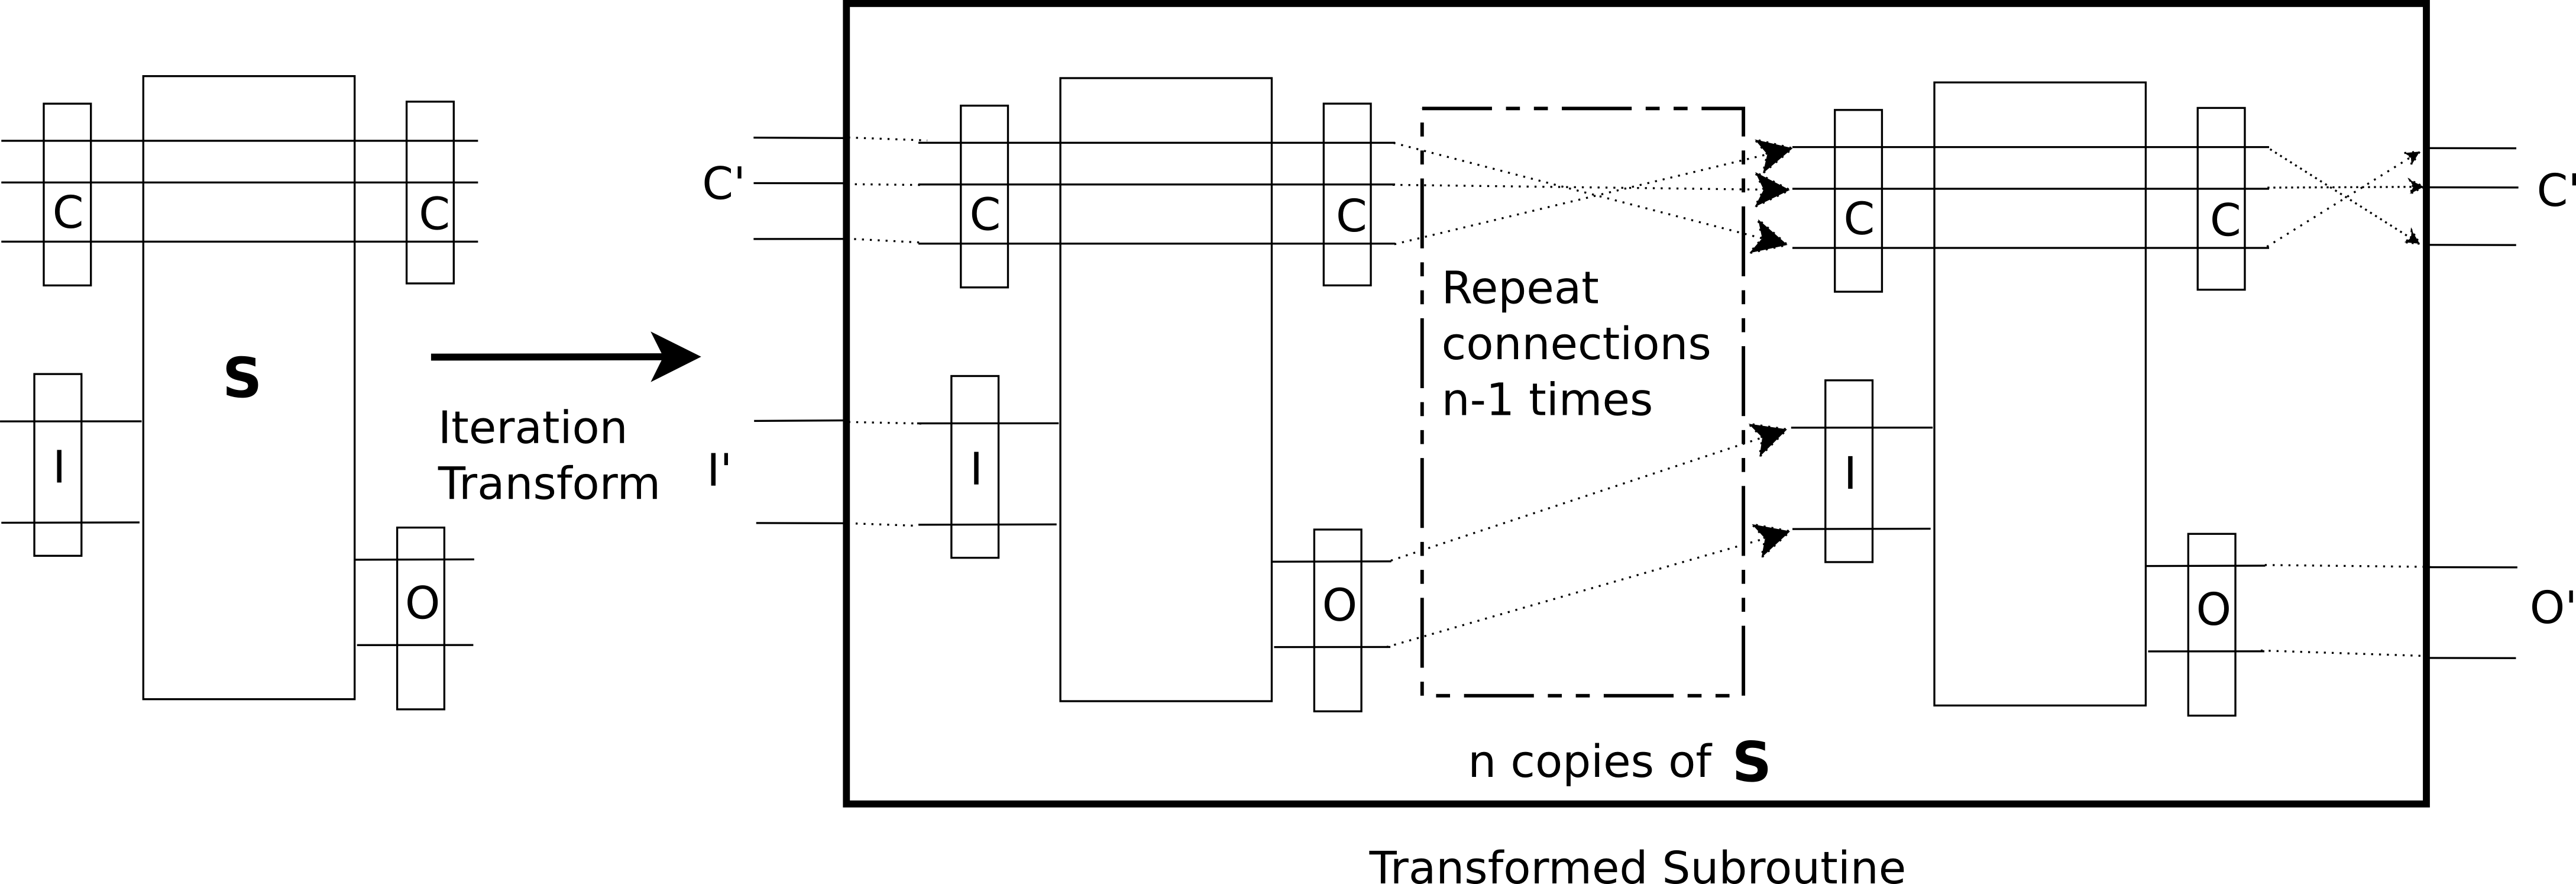
\includegraphics[scale=.4]{diagrams/SubroutineIterationTransform.png}
   \caption{Transforming a subroutine to an iterated subroutine}
   \label{fig:transforming_a_subroutine_to_an_iterated_subroutine}
\end{figure}
% subsection iteration_transformation_of_a_subroutine (end)

\subsection{Folding subroutines} % (fold)
\label{sub:folding_subroutines}

In addition to the concept of iteration the ability to fold
subroutines over data structures could also be useful. A
folded call of a subroutine is similar to an iteration, in
that controls and possibly some of the inputs
and outputs are iterated. The difference occurs in that we
expect to take some of the inputs from a data structure and
return some of the outputs to a data structure. An example of
this would be folding over a list of \qubit{s} where
each qubit is taken as a input for each iteration.

First, we will examine the requirements for a non-linear
safe fold, that is, where no input duplication on the
control wires is allow



\begin{definition}\label{def:linear_only_subroutine_fold}
  Given a subroutine $S=([gate],C,I,O,c,r,n)$, a starting context of
  typed wires $W_1$ and a data structure on wires $D\subset W_1$, a
  \emph{linear-only folded call} of $S$ over $D$ resulting in the context
  of typed wires $W_2$ and the data structure $E\subset W_2$ consists of the
  tuple $(CI_f,CO_f,  g, h, ciof_b, s_{in}, s_{out})$ where
  \begin{itemize}
    \item $CI_f::\type{Arity}, \dom{CI_f} \subset \dom{C}\cup \dom{I}$,
    \item $CO_f::\type{Arity}, \dom{CO_f} \subset \dom{C}\cup \dom{O}$,
    \item $g:\dom{C}\cup\dom I / \dom{CI_f} \to W_1$ and $g$ is injective,
    \item $h:\dom{C}\cup\dom O /\dom{CO_f} \to W_2$ and $h$ is injective
    \item $ciof_b$ is a bijection between $(\dom{C}\cup\dom{O})/\dom{CO_f}$
      and $(\dom{C}\cup\dom{I})/\dom{CI_f}$,
    \item $s_{in}: \dom{CI_f} \to W_1$ (pulls from $D$),
    \item $s_{out}: \dom{CO_f} \to W_2$ (pushes to $E$),
    \item $g + s_{in} \in F(\nothing,I,W_1)$,
    \item $ciof_b^{-1} + s_{in} \in F(\nothing,I,W_1)$,
    \item $ciof_b + s_{out} \in F(\nothing,O,W_2)$,
    \item $h + s_{out} \in F(\nothing,O,W_2)$,
    \item $|\dom{CI_f}| = leafsize(D)$,
    \item $leafsize(E) = |\dom{CO_f}|$.
  \end{itemize}
\end{definition}

\begin{definition}\label{def:structured_linear_folded_call}
  Given the data for an linear-only folded call,
  a \emph{structured linear-only folded call} is a pair of high level
  structures $(i_s,o_s)$ and $(i_{fs},o_{fs})$  and a pair of quantum
  terms $(a,b)$ such that:
  \begin{itemize}
    \item $i_s(a) = g + s_{in}$,
    \item $o_s(h + s_{out}) = b$,
    \item $i_{fs}(a) = s_{in}$, and
    \item $o_{fs}(s_{out}) = b$.
  \end{itemize}

\end{definition}

Discussion points:
\begin{itemize}
  \item Does the structured call get rid of the last two items regarding
  leafsize?  Same issue with non-linear safe call.
  \item For the structured call, it appears to me that there is only
  one pair of terms $a,b$ with two different (de)structuring morphisms.
\end{itemize}

The action on the wires of the calling program will be given by this relation:
\[
s_{out} + h \circ (s_{out} + cio_f + s_{in})^{len(D)}
\circ (g + s_{in})^{-1}.
\]
\begin{example}[Fold over Carry]\label{ex:fold_over_carry}
\end{example}

For this example, we use the carry portion of the addition algorithm found
in \cite{Vedral:1995ga}.

The carry circuit is shown below:
\[\Qcircuit @C=1em @R=.7em {
\lstick{anc} & \ctrl{2} & \qw & \qw & \rstick{anc} \qw \\
\lstick{a}  & \qw & \ctrl{1} & \ctrl{1} & \rstick{a} \qw \\
\lstick{b}  & \ctrl{1} & \targ & \ctrl{1} & \rstick{b} \qw \\
\lstick{c}  & \targ & \qw& \targ & \rstick{c} \qw
}
\]

The intent of this circuit is to compute the final carry when
adding the quregisters $A$ and $B$. The input prepares
the $anc$ in state $\ket{0}$ and an auxiliary register $R$,
the same size as $A$ and $B$ as $\ket{00\ldots0}$. Assume
that $A = [w_1,w_2,w_3], B=[w_4,w_5,w_6], anc=w_7$ and
$R=[w_8,w_9,w_{10}]$. $(A,B,R)$, a tuple of three registers
forms our $D$ --- the input to the fold. Then,
we may perform a folded call of carry as follows:
\begin{itemize}
  \item $\dom{C} = \{anc,a\},\ \dom{I} = \{b,c\} = \dom{O}$;
  \item $\dom{CI_f} = \{a,b,c\}$ and $\dom{CO_f} = \{anc,a,b\}$;
  \item $g = \{anc \mapsto w_{6}\}$, $h=\{c\mapsto w_{10}\}$
  \item $ciof_b = \{c \mapsto anc \}$
  \item $s_{in} = \{a \mapsto D[0], b \mapsto D[1], c \mapsto D[2]\}$
  \item $s_{out} = \{anc \mapsto E[2], a \mapsto E[0], b \mapsto E[1]\}$.
\end{itemize}
From the mapping $s_{out}$, we set $E = (A,B,R')$ where $R'=[w_7,w_8,w_9]$.

Discussion points:
\begin{itemize}
  \item Is there a non-linear safe use case? Carry seemed quite simple,
    but it required linear safe inputs when folded.
  \item Each fold iteration input might be multiple \qubit{s},
  combined into a single data structure, as in 
    \vref{ex:fold_over_carry}.
  \item The number of inputs and outputs no longer need
    to agree as they did in iteration.  An example would be a subroutine that
    applied a two \qubit gate and then discarded one of the \qubits.
    The fold would be expected to convert a list of pairs  of \qubit{s}
    to a list of \qubit{s}. (Note this subroutine would not be reversible
    or controllable).
  \item The shape of the foldable in and out as well as the number of \qubits
    at each leaf would need to be known.
  \item The $F(C,K,W)$ permissible functions are not quite right for
    linear-only folds --- we do not want to allow duplication of any of
    the inputs, so $F(C,K,W)$ becomes $F(\nothing,C+K,W)$.
\end{itemize}

\begin{definition}\label{def:subroutine_fold}
  Given a subroutine $S=([gate],C,I,O,c,r,n)$, a starting context of
  typed wires $W_1$ and a data structure on wires $D\subset W_1$, a
  \emph{folded call} of $S$ over $D$ resulting in the context of typed wires
  $W_2$ and the data structure $E\subset W_2$ consists of the tuple
  $(I_f,O_f, f_{in}, f_{out}, g, h, c_b, iof_b, s_{in}, s_{out} )$ where
  \begin{itemize}
    \item $I_f::\type{Arity}, \dom{I_f} \subset \dom{I}$,
    \item $O_f::\type{Arity}, \dom{O_f} \subset \dom{O}$,
    \item $f_{in}:\dom C \to W_1\cup W_2$
    \item $f_{out}:\dom C \to W_1\cup W_2$
    \item $g:\dom I / \dom{I_f} \to W_1$
    \item $h:\dom O /\dom{O_f} \to W_2$
    \item $c_b$ is a bijection (permutation) of $C$,
    \item $iof_b$ is a bijection between $\dom{O}/\dom{O_f}$
      and $\dom{I}/\dom{I_f}$,
    \item $s_{in}: \dom{I_f} \to W_1$ (pulls from $D$)
    \item $s_{out}: \dom{O_f} \to W_2$ (pushes to $E$)
    \item $f_{in}+ g+ s_{in} \in F(C,I,W_1)$,
    \item $f_{out}+ h + s_{out} \in F(C,O,W_2)$,
    \item $iof_b + s_{in} \in F(\nothing,I,W_1)$,
    \item $iof_b + s_{out} \in F(\nothing,O,W_2)$,
    \item $|\dom{I_f}| = leafsize(D)$
    \item $leafsize(E) = |\dom{O_f}|$
  \end{itemize}

\end{definition}

\begin{definition}\label{def:structured_folded_call}
  Given the data for an folded call,
  a \emph{structured folded call} is a pair of high level structures
  $(i_s,o_s)$ and $(i_{fs},o_{fs})$  and a pair of quantum
  terms $(a,b)$ such that:
  \begin{itemize}
    \item $i_s(a) = f_{in}+g + s_{in}$,
    \item $o_s(f_{out} + h + s_{out}) = b$,
    \item $i_{fs}(a) = s_{in}$, and
    \item $o_{fs}(s_{out}) = b$.
  \end{itemize}

\end{definition}

% subsection folding_subroutines (end)

\subsection{Subroutine to folded subroutine transform} % (fold)
\label{sub:subroutine_to_folded_subroutine_transform}

In order to transform a given subroutine, we require the following data:
\begin{itemize}
  \item A bijection from some subset of the control and output wires to some
  subset of the control and input wires;
  \item a count of the number of iterations.
\end{itemize}

This allows us to derive a new $C,I,O$ for the fold subroutine. We proceed
with the formal definition.
\begin{definition}\label{def:fold_transform_of_a_subroutine}
  The \emph{fold transform} of a subroutine is a function $S_f$ with
  parameters $(n,b_{cio})$ which takes the subroutine $(gates,C,I,O,r,c,n)$
  to the subroutine $(gates',C',I',O',r,c,n)$.
  The parameters have the following types:
  \begin{align*}
    n&::\type{Int}, n>0;\\
    b_{cio}&::\type{bijection(CI \leftrightarrow CO)} \\
      &\text{where }CI\subseteq C\cup I\text{ and }\subseteq C\cup O.
  \end{align*}
\end{definition}

Note that $b_{cio}$ may be defined as a set of ordered pairs
\begin{equation}
  \{(f,t)|f\in C\cup I, t \in C\cup O,\text{ and } f,t \text{ appear at most once}\}.
  \label{eq:defintion_of_bcio}
\end{equation}
The data we need to create for the end result are the set of control wires,
the input and output wires and the new gates sequence. We proceed with
presenting the algorithm for the control wires.

When considering which inputs (and hence outputs) are control wires in the
transformed subroutine, we must follow the path of a control input. A control
input to the base subroutine will remain a control input to the transformed
subroutine only if its full folded path contains only control wires before
exiting. Depending upon the structure of $b_{cio}$ it is possible all, none
or some finite subset of specific control wires become controls for the
transformed routine.

To determine if a wire is a control, we will calculate a characteristic of the
wire and show that it requires at most $k$ iterations to calculate, where
$k$ is the number of control wires of the original subroutine.

First, define:
\begin{align*}
  \Omega &:: C \to C \cup \{*,@\}\\
  \Omega(c) &=
    \begin{cases}
      c'&\text{if }b_{cio}(c) = c'\text{ and }c'\in C,\\
      *&\text{if $c$ is not the first element of any pair in }b_{cio},\\
      @&\text{if }b_{cio}(c) = j\text{ and }j\in I.
    \end{cases}
\end{align*}
Then, noting that $k = |C|$, define:
\begin{align*}
  \Gamma &:: C \to \nat \cup \{\infty\}\\
  \Gamma(c) &=
  \begin{cases}
    \infty & \Omega(c) = *,\\
    0 & \Omega(c) = @,\\
    1 + \Gamma(\Omega(c)) & \Gamma(\Omega(c)) < k,\\
    \infty & \Gamma(\Omega(c)) \ge k.
  \end{cases}
\end{align*}

Dually, we may define functions  $\Theta(c)$ and $\Delta(c)$:
\begin{align*}
\Theta &:: C \to C \cup \{*,@\}\\
\Theta(c) &=
  \begin{cases}
    c'&\text{if }b_{cio}(c') = c\text{ and }c'\in C,\\
    *&\text{if $c$ is not the second element of any pair in }b_{cio},\\
    @&\text{if }b_{cio}(o) = c\text{ and }o\in O.
  \end{cases}\\
  \Delta &:: C \to \nat \cup \{\infty\}\\
  \Delta(c) &=
  \begin{cases}
    \infty & \Theta(c) = *,\\
    0 & \Theta(c) = @,\\
    1 + \Delta(\Theta(c)) & \Delta(\Theta(c)) < k,\\
    \infty & \Delta(\Theta(c)) \ge k.
  \end{cases}
\end{align*}

Note that in the case of cycles among control wires, the cycle \emph{must} be
of size $k$ or less. As such, at most $k$ iterations of $\Gamma$ are required
before confirming a value for $\Gamma(c)$. The same argument applies to
computing $\Theta$.

Assuming that $C$ is ordered, the data for $b_{cio}$ may be stored such that
computing $b_{cio}(c)$ and therefore $\Omega(c)$ is of $\BigO{\log k}$.
Therefore, $\Gamma$ is of complexity $\BigO{k\log k}$ and computing
$\Gamma$ for all of $C$ will then be of $\BigO{k^2 \log k}$. Computing
$\Delta$ will have the same complexity.

We may now describe the  algorithm for determining control wires, $C'$
input wires, $I'$ and output wires, $O'$ of the transformed subroutine.
In the algorithm, $n$ is the number of iterations, $k$ is the cardinality
of $C$. Additionally, we compute a \emph{rank} of each $c$ in $C'$. The
\emph{rank} of $c$ is the number of iterations that $c$ will go through.
\begin{enumerate}
  \item Add all members of $I$ to $I'$, subscripting with $1$.
  \item For all $i\in I$ where $i \nin \rng b_{cio}$, add
    $i_2,i_3,\ldots,i_n$ to $I'$.
  \item Add all members of $O$ to $O'$, subscripting with $n$.
  \item For all $o\in O$ where $o \nin \dom b_{cio}$, add
    $o_1,o_2,\ldots,o_{n-1}$ to $O'$.
  \item Partition $C$ into four subsets:
  \begin{align*}
    C_*    &= \{c|c\nin \dom b_{cio}\text{ and }c\nin \rng b_{cio}\},\\
    C_d    &= \{c|c\in \dom b_{cio}\text{ and }c\nin \rng b_{cio}\},\\
    C_r    &= \{c|c\nin \dom b_{cio}\text{ and }c\in \rng b_{cio}\},\\
    C_{dr} &= \{c|c\in \dom b_{cio}\text{ and }c\in \rng b_{cio}\}.
  \end{align*}
  \item For each $c\in C_*$, add $c_1,c_2,\ldots,c_n$ to $C'$. Set the
    rank of each of these to $0$.
  \item For each $c\in C_d$, compute $j=\Gamma(c)$. If $j \ge n$, add
    $c_1,c_2,\ldots,c_n$ to $C'$. If not, then:
    \begin{itemize}
      \item Add $c_{n-j},c_{n-j+1},\ldots,c_n$ to $C'$, setting the
        rank of $c_\ell$ to $n-\ell$.
      \item Add $c_1,c_2,\ldots,c_{n-j-1}$ to $I'$.
    \end{itemize}
  \item For each $c\in C_r$, compute $m=\Delta(c)$. If $m \ge n$, add
    $c_1,c_2,\ldots,c_n$ to $C'$, setting each item to rank $0$.
    If not, then:
    \begin{itemize}
      \item Add $c_1,c_2,\ldots,c_{j+1}$ to $C'$, setting each rank to $0$.
      \item Add $c_{j+2},c_{j+3},\ldots,c_{n}$ to $I'$.
    \end{itemize}
  \item For each $c\in C_{dr}$, compute $j=\Gamma(c), m=\Delta(c)$. Then
    if $j>n-1$, add $c_1$ to $C'$, setting its rank to $n-1$, otherwise
    add it to $I'$. Conversely, if $m>n-1$, add $c_n$ to $C'$, setting its
    rank to $0$, otherwise add it to $O'$. In the case
    where both $c_1$ and $c_n$ are added to $C'$, we have actually added
    one too many items to $C'$ as there will be a duplication. This is
    addressed in the final step, where the in-out names of the control
    wires are reconciled.
  \item Reconcile the $C'$ names: For each $c_h\in C'$, compute
    $x=b_{cio}^{Rank(c)}(c)$. In $C'$, replace $x_n$ with $c_h$. After
    completing this computation, remove any duplicates.
\end{enumerate}

% The above algorithm will compute the correct $C'$ and $I'$ for the transformed
% subroutine. Additionally, we must also compute the matching of the control
% wires on input and output. To do this, we must essentially trace the path
% of each of the wires in $C'$ and determine what is the final output. There
% are three cases to consider for each $c$:
% \begin{itemize}
%   \item $\Gamma(c_m) = j>0$. This means that $c_m$ is an input with $j$ or
%     fewer iterations remaining. Compute $c' = \Omega^{rank(c_m)}(c)$. The name
%     matched with $c_m$ is then $c'_{m+rank(c_m)}$.
%   \item $\Gamma(c) = \infty, \Omega(c)=*$. $c$ is an immediate in/out control
%     wire.
%   \item $\Gamma(c) = \infty, \Omega(c)=c'$. This case occurs when $c$ is part
%     of a cycle. As noted above, the cycle must be of length $j \le k$. Hence,
%     compute $c_{\ell}=\Omega^{\ell}(c)$ where $\ell=n-1 \mod j$. Then
%     $c_\ell$ is the name of the output matched with $c$.
% \end{itemize}


% subsection subroutine_to_folded_subroutine_transform (end)
\subsection{Examples of folding} % (fold)
\label{sub:examples_of_folding}

\begin{example}\label{exmpl:fold_example_with_three_mixed_in_out}
  Consider $S=(\_,\{a,b\},\{c\},\{d\},\_,\_,\_)$ and $b_{cio}=\{(a,c),(b,a)\}$
  and an iteration count of $3$. See 
  \vref{fig:Fold_with_extra_in_out}.
\end{example}
\begin{figure}[htbp]
  \centering
    \[
\Qcircuit{
 & \dqw& \dqw &\dqw &\dqw &\dqw\ar@{.} [dddr]&\\
 & \dqw& \dqw\ar@{.}[ddr]\\
 & \multigate{3}{S_1}_{a_1} & \qw  \ar@{.}[dddr] &  & \multigate{3}{S_2}_{a_2}&\qw\ar@{.}[dddr]&  & \multigate{3}{S_3}_{a_3}&\qw\\
 & \ghost{S_1}_{b_1} & \qw \ar@{.}[ur]& &\ghost{S_2}_{b_2}&\qw\ar@{.}[ur]& &\ghost{S_3}_{b_3}&\qw\\
 &  & & & & & & & & & &\\
 & \ghost{S_1}_{c_1}& \qw_{d_1} \ar@{.}[ddr]& &\ghost{S_2}_{c_2}&\qw_{d_2}\ar@{.}[dr]& &\ghost{S_3}_{c_3}&\qw_{d_3}\\
 &            &                & &            &              & &\dqw&\dqw\\
 &            &                & & \dqw      &\dqw           &\dqw&\dqw&\dqw
}
\]
  \caption{Fold with extra in/out}
  \label{fig:Fold_with_extra_in_out}
\end{figure}

From the data, we compute:
\begin{align*}
  \Omega(a) &= @\text{ and }\Omega(b) = a,\\
  \Gamma(a) &=0\text{ and }\Gamma(b) = 1,\\
  \Theta(b) &=*\text{ and }\Delta(b)=\infty,\\
  \Theta(a)=b\text{ and } \Delta(a)=\infty.
\end{align*}

Now, following the steps of the algorithm,
\begin{enumerate}
  \item $I' \mapsto \{c_1\}$.
  \item No change to $I'$.
  \item $O' \mapsto \{d_3\}$.
  \item $O' \mapsto \{d_1,d_2,d_3\}$.
  \item $C_*=\nothing, C_d=\{b\}, C_r =\nothing, C_{dr}=\{a\}$.
  \item For $C_d$, As $\Gamma(b)=1$, we have $C' \mapsto \{b_2,b_3\}$ and
    $I' \mapsto \{c_1,b_1\}$. The rank of $b_2$ is 1 and the rank of $b_3$
    is 0.
  \item For $C_{dr}=\{a\}$, $\Gamma(a)=0$ and $\Delta(a)=\infty$, therefore
    we add $a_1$ to $I'$ and $a_3$ to $C'$. The rank of $a_3$ is zero.
    At this stage, we now have
    $I'=\{c_1,b_1,a_1\}, O'=\{d_1,d_2,d_3\}$ and $C'=\{b_2,b_3,a_3\}$.
  \item Reconcile $C'$: $b_{cio}(b)=a$ and $b_{cio}(a)=c$, therefore
    $b_{cio}^1(b_2)=a_3$, $b_{cio}^0(b_3)=b_3$, and $b_{cio}^0(a_3)=a_3$.
    Following our replacement scheme, $C'=\{b_2,b_3\}$.
\end{enumerate}

Hence our final result is:
\begin{align*}
  I'&=\{c_1,b_1,a_1\},\\
  O'&=\{d_1,d_2,d_3\}\text{ and}\\
  C'&=\{b_2,b_3\}.
\end{align*}

\begin{example}\label{exmpl:fold_example_with_partial_bcio}
  Consider $S=(\_,\{a,b\},\{c\},\{d\},\_,\_,\_)$ as in 
  \vref{exmpl:fold_example_with_three_mixed_in_out} and
  $b_{cio}=\{(a,c),(b,a),(d,b)\}$ and an iteration count of $3$. See 
  \vref{fig:Fold_with_three_iterations}.
\end{example}
\begin{figure}[htbp]
  \centering
    \[
\Qcircuit{
 & \multigate{3}{S_1}_{a_1} & \qw  \ar@{.}[dddr] &  & \multigate{3}{S_2}_{a_2}&\qw\ar@{.}[dddr]&  & \multigate{3}{S_3}_{a_3}&\qw\\
 & \ghost{S_1}_{b_1} & \qw \ar@{.}[ur]& &\ghost{S_2}_{b_2}&\qw\ar@{.}[ur]& &\ghost{S_3}_{b_3}&\qw\\
 &  & & & & & & & & & &\\
 & \ghost{S_1}_{c_1}& \qw_{d_1} \ar@{.}[uur]& &\ghost{S_2}_{c_2}&\qw_{d_2}\ar@{.}[uur]& &\ghost{S_3}_{c_3}&\qw_{d_3}\\
}
\]
\caption{Fold with three iterations}
  \label{fig:Fold_with_three_iterations}
\end{figure}

From the data, we have:
\begin{align*}
  \Omega(a) &= @\text{ and }&\Gamma(a)=0,\\
  \Omega(b) &= a\text{ and }&\Gamma(b) = 1,\\
  \Theta(b)&=@\text{ and }&\Delta(b)=0,\\
  \Theta(a)&=b\text{ and }&\Delta(a)=1.
\end{align*}

Now, following the steps of the algorithm,
\begin{enumerate}
  \item $I' \mapsto \{c_1\}$.
  \item No change to $I'$.
  \item $O' \mapsto \{d_3\}$.
  \item All $o$ are in the range of $b_{cio}$, therefore no further
    change to $O'$.
  \item $C_*=C_d=C_r = \nothing, C_{dr}=\{a,b\}$.
  \item As $n-1=2 > \Gamma(a),\Gamma(b)$, we have $I'
    \mapsto \{c_1,a_1,b_1\}$. Similarly, since $n-1=2 > \Delta(a),\Delta(b)$,
    $O'\mapsto \{a_3,b_3,d_3\}$
  \item With $C'$ empty, there are no further steps.
\end{enumerate}
Hence our final result is:
\begin{align*}
  I'&=\{c_1,b_1,a_1\},\\
  O'&=\{a_3,b_3,d_3\}\text{ and}\\
  C'&=\nothing.
\end{align*}

\begin{example}\label{exmpl:fold_transform_example_of_carry}
  Consider $C=(\_,\{r,a\},\{b,c\},\{d,e\},\_,\_,\_)$,
  $b_{cio}=\{(e,r)\}$ and an iteration count of $4$. See 
  \vref{fig:fold_carry_transformed}.
\end{example}
\begin{figure}[htbp]
  \centering
    \[
\xymatrix @R=7pt @*=<0em>{
 & \multigate{3}{C}_{r_1} & \qw& \qw & \qw & \qw & \qw & \qw & \qw\\
 & \ghost{C}_{a_1} & \qw       & \qw & \qw & \qw & \qw & \qw & \qw\\
 & \ghost{C}_{b_1} & \qw_{d_1} & \qw & \qw & \qw & \qw & \qw & \qw\\
 & \ghost{C}_{c_1} & \qw_{e_1} & \multigate{3}{C}_{r_2} & \qw & \qw & \qw & \qw  & \qw\\
 & \qw_{a_2}       & \qw       & \ghost{C} & \qw        & \qw & \qw & \qw & \qw\\
 & \qw_{b_2}       & \qw       & \ghost{C} & \qw_{d_2}  & \qw & \qw & \qw & \qw \\
 & \qw_{c_2}       & \qw       & \ghost{C} & \qw_{e_2}  & \multigate{3}{C}_{r_3} &\qw& \qw & \qw\\
 & \qw_{a_3}       & \qw       & \qw       & \qw        & \ghost{C} &\qw      & \qw & \qw \\
 & \qw_{b_3}       & \qw       & \qw       & \qw        & \ghost{C} &\qw_{d_3}& \qw & \qw\\
 & \qw_{c_3}       & \qw       & \qw       & \qw        & \ghost{C} &\qw_{e_3}& \multigate{3}{C}_{r_4} &\qw\\
 & \qw_{a_4}       & \qw       & \qw       & \qw        & \qw       & \qw     & \ghost{C} &\qw\\
 & \qw_{b_4}       & \qw       & \qw       & \qw        & \qw       & \qw     & \ghost{C} &\qw_{d_4}\\
 & \qw_{c_4}       & \qw       & \qw       & \qw        & \qw       & \qw     & \ghost{C} &\qw_{e_4}\\
}
\]
  \caption{Fold of Carry}
  \label{fig:fold_carry_transformed}
\end{figure}

From the data, we have:
\begin{align*}
  \Omega(r) &= *\text{ and }&\Omega(a) = *,\\
  \Gamma(r)&=\infty\text{ and }&\Gamma(a) = \infty,\\
  \Theta(r)&=@\text{ and }&\Delta(r)=0,\\
  \Theta(a)=*\text{ and } &\Delta(a)=\infty.
\end{align*}

Now, following the steps of the algorithm,
\begin{enumerate}
  \item $I' \mapsto \{b_1,c_1\}$.
  \item No element of $I$ appears in $b_{cio}$, therefore we now have
    $I' \mapsto \{b_1,c_1,b_2,c_2,b_3,c_3,b_4,c_4\}$
  \item $O' \mapsto \{d_4,e_4\}$.
  \item Only $e$ is in the range of $b_{cio}$, therefore we add
  $d_1,d_2,d_3$ to  $O'$, giving us $\{d_1,d_2,d_3,d_4,e_4\}$.
  \item $C_*=\{a\},C_d=\nothing, C_r = \{r\},\ C_{dr}=\nothing$.
  \item Considering $C_*$, we add $\{a_1,a_2,a_3,a_4\}$ to $C'$, each with
    rank 0.
  \item Next considering $C_r$, as $\Delta(r)=0$, we add $r_1$ to $C'$ with
    rank 0 and then add $r_2,r_3,r_4$ to $O'$.
  \item As each element of $C'$ is of rank 0, there is no changes
    to the names.
\end{enumerate}

Hence our final result is:
\begin{align*}
  I'&=\{b_1,c_1,b_2,c_2,b_3,c_3,b_4,c_4\},\\
  O'&=\{d_1,d_2,d_3,d_4,e_4,r_2,r_3,r_4\}\text{ and}\\
  C'&=\{r_1,a_1,a_2,a_3,a_4\}.
\end{align*}

% subsection examples_of_folding (end)
% section subroutine_calls_and_transformers (end)

% section diagram_of_folded_carry (end)
\section{Alternate Algorithm for Fold Transformation} % (fold)
\label{sec:alternate_algorithm_for_fold_transformation}
In  this section, we present an alternate algorithm for calculating the
type and names of control, input and output wires for a folded
subroutine.  The starting point is 
\vref{def:fold_transform_of_a_subroutine}
and the ordered pairs of $b_{cio}$: A set of ordered pairs
$\{(f,t)|f\in C\cup I, t \in C\cup O\}$.

To implement the algorithm of calculating the folded subroutines $C,I$ and
$O$, we need the following:
\begin{itemize}
  \item $I\cap O = \nothing$, which may be accomplished by renaming if needed.
  \item We create the sets $C_j,I_j,O_j$ for $j=1\ldots n$ where the members
    of $X_j$ are the elements of $X$ together with the subscript $j$ where
    $X$ is one of $C,I,O$.
\end{itemize}

The algorithm proceeds by creating a set of ``type'' constraints for each of
the elements of the new sets, based upon $b_{cio}$ and membership in a $C,I$
or $O$ set.

The algorithm steps are:
\begin{enumerate}
  \item Create a set $\mathcal{C}$ of pairs $(a_j,b_{j+1})$ for $j$
  ranging from $0$ to $n-1$ based upon the bijection $b_{cio}$.
  \item For each $j=0\ldots n-1$,
  \begin{enumerate}
    \item For all $c\in C_j$, if $(c,\_)\notin\mathcal{C}$,
      add the pair $(c,\nothing)$
    \item For all $c\in C_j$, if $(\_,c)\notin\mathcal{C}$,
      add the pair $(\nothing,c)$
    \item For all $o\in O_j$, if $(o,\_)\notin\mathcal{C}$,
      add the pair $(o,\nothing)$
    \item For all $i\in I_j$, if $(\_,i)\notin\mathcal{C}$,
      add the pair $(\nothing,i)$
  \end{enumerate}
  \item Convert the pairs in $\mathcal{C}$ to equations and constraints as
    follows for each pair $(a,b)$:
  \begin{enumerate}
    \item $a=\nothing\implies \begin{cases}
      b::(b,C)&\text{when }b\in C_j\text{for some }j,\\
      b::(b,I)&\text{when }b\in I_j\text{for some }j.
    \end{cases}$
    \item $a\in C_{j-1}\implies \begin{cases}
      b=a&\text{when }b\in C_j,\\
      b=a, b::I&\text{when }b\in I_j,\\
      a::(C,a)&\text{when }b=\nothing.
    \end{cases}$
    \item $a\in O_{j-1}\implies \begin{cases}
      b=a, b::O&\text{when }b\in C_j,\\
      \text{no equation}&\text{when }b\in I_j,\\
      a::(O,a)&\text{when }b=\nothing.
    \end{cases}$
  \end{enumerate}
  \item Solve the equations with the constraints, with the assumption that
    \[\xymatrix{
      &C\ar[dl]\ar[dr] \ar[d] & \\
      I \ar[dd]&(C,b)\ar[dr] \ar[d]&O\ar[d] \\
      &(b,C)\ar[dl]& (O,b) \\
      (b,I)& & }
    \]
  For example,
  \begin{itemize}
    \item $a::O, a::C$ is solvable with $a::O$;
    \item $a=b,b::(b,C),a::I$ is solved by $b,a::(b,I)$;
    \item $a=b, b=d, a::(a,C), d::(C,d)$ is solved by $a,b,d::(a,C)$.
  \end{itemize}
  \item For the folded subroutine, $X$ will be all items of ``type'' $X$,
    where $X$ is any of $C,I,O$, the names of each entry will be the companion
    name with the ``type''.
\end{enumerate}
\note{The algorithm above works correctly, but likely has too high of a
complexity, depending on the number of iterations. Need to revise in the
next version to see if we can make the complexity proportional to the number
of wires in/out.}
\subsection{Examples of folding with Alternate Algorithm} % (fold)
\label{sub:examples_of_folding_with_alternate_algorithm}
\begin{example}\label{exmpl:alternate_fold_example_with_three_mixed_in_out}
  We repeat \vref{exmpl:fold_example_with_three_mixed_in_out}, that is,
  $S=(\_,\{a,b\},\{c\},\{d\},\_,\_,\_)$ and $b_{cio}=\{(a,c),(b,a),(d,b)\}$
  and an iteration count of $3$. See 
  \vref{fig:Fold_with_three_iterations}.
\end{example}
There are two control wires $a,b$, an input wire $d$ and one output
wire $d$. We  will do three iterations. Our set $\mathcal{C}$ of pairs
becomes:
\begin{align*}
  \{ & (\nothing,a),\ (\nothing,b),\ (\nothing,c),\\
  & (b,a_1),\ (d,b_1),\ (a,c_1),\\
  & (b_1,a_2),\ (d_1,b_2),\ (a_1,c_2),\\
  & (a_2,\nothing),\ (b_2,\nothing),\ (c_2,\nothing)\}.\\
\end{align*}
Translating each of these to equations and constraints, we get:
\begin{align*}
  &a::(a,C), b::(b,C), c::(c,I)\\
  &b=a_1, b_1=d\ b_1::O, a=c_1\ c_1::I\\
  &b_1=a_2, b_2=d_1\ b_2::O, a_1=c_2\ c_2::I\\
  &a_2::(C,a_2), b_2::(C,b_2), d_2::(O,d_2)
\end{align*}
As we have three wires in and three wires out, we expect to see six separate
groupings in the solution to the above equations. We will proceed by starting
from the top left.
\begin{align*}
  \text{start: }a &\quad a=c_1, ::I, ::(a,C) &\implies a::(a,I)\\
  \text{start: }b &\quad  b=a_1,a_1=c_2, ::I, ::(b,C) &\implies b::(b,I)\\
  \text{start: }c &\quad  ::(c,I) &\implies c::(c,I)\\
  \text{start: }b_1 &\quad  b_1=d, b_1=a_2, ::O, ::(C,a_2) &\implies
    a_2::(O,a_2)\\
  \text{start: }b_2 &\quad  b_2=d_1, ::O, ::(C,b_2) &\implies b_2::(O,b_2)\\
  \text{start: }d_2 &\quad  ::(O,d_2) &\implies d_2::(O,d_2)
\end{align*}
% subsection examples_of_folding (end)
% section alternate_algorithm_for_fold_transformation (end)



\begin{singlespace}
\bibliography{bibentries-phd}
\bibliographystyle{plain}
\end{singlespace}
\appendix
%%\fancyhead[RO,LE]{\thepage}
%\fancyfoot{} 

\chapter{First Appendix}

%Start the body text
Lorem ipson dolor sic amet sec in consetum epsom nunc ad valorem. Lorem ipson dolor sic amet
sec in consetum nunc ad valorem. Lorem epsom ipson dolor sic amet sec in consetum nunc ad valorem. 
Lorem ipson dolor sic amet sec in consetum nunc ad valorem. Lorem ipson dolor sic amet
sec in consetum nunc ad valorem. Lorem ipson dolor sic amet sec in epsom consetum nunc ad valorem.

Lorem ipson dolor sic amet sec in consetum epsom nunc ad valorem. Lorem ipson dolor sic amet
sec in consetum nunc ad valorem. Lorem epsom ipson dolor sic amet sec in consetum nunc ad valorem. 
Lorem ipson dolor sic amet sec in consetum nunc ad valorem. Lorem ipson dolor sic amet
sec in consetum nunc ad valorem. Lorem ipson dolor sic amet sec in epsom consetum nunc ad valorem.
Lorem ipson dolor sic amet sec in consetum epsom nunc ad valorem. Lorem ipson dolor sic amet
sec in consetum nunc ad valorem. Lorem epsom ipson dolor sic amet sec in consetum nunc ad valorem. 
Lorem ipson dolor sic amet sec in consetum nunc ad valorem. Lorem ipson dolor sic amet
sec in consetum nunc ad valorem. Lorem ipson dolor sic amet sec in epsom consetum nunc ad valorem.
Lorem ipson dolor sic amet sec in consetum epsom nunc ad valorem. Lorem ipson dolor sic amet
sec in consetum nunc ad valorem. Lorem epsom ipson dolor sic amet sec in consetum nunc ad valorem. 
Lorem ipson dolor sic amet sec in consetum nunc ad valorem. Lorem ipson dolor sic amet
sec in consetum nunc ad valorem. Lorem ipson dolor sic amet sec in epsom consetum nunc ad valorem.

Lorem ipson dolor sic amet sec in consetum epsom nunc ad valorem. Lorem ipson dolor sic amet
sec in consetum nunc ad valorem. Lorem epsom ipson dolor sic amet sec in consetum nunc ad valorem. 
Lorem ipson dolor sic amet sec in consetum nunc ad valorem. Lorem ipson dolor sic amet
sec in consetum nunc ad valorem. Lorem ipson dolor sic amet sec in epsom consetum nunc ad valorem.
Lorem ipson dolor sic amet sec in consetum epsom nunc ad valorem. Lorem ipson dolor sic amet
sec in consetum nunc ad valorem. Lorem epsom ipson dolor sic amet sec in consetum nunc ad valorem. 
Lorem ipson dolor sic amet sec in consetum nunc ad valorem. Lorem ipson dolor sic amet
sec in consetum nunc ad valorem. Lorem ipson dolor sic amet sec in epsom consetum nunc ad valorem.
\begin{figure}
Place the figure here
\caption{Figure in the appendix}
\end{figure}

Lorem ipson dolor sic amet sec in consetum epsom nunc ad valorem. Lorem ipson dolor sic amet
sec in consetum nunc ad valorem. Lorem epsom ipson dolor sic amet sec in consetum nunc ad valorem. 
Lorem ipson dolor sic amet sec in consetum nunc ad valorem. Lorem ipson dolor sic amet
sec in consetum nunc ad valorem. Lorem ipson dolor sic amet sec in epsom consetum nunc ad valorem.
Lorem ipson dolor sic amet sec in consetum epsom nunc ad valorem. Lorem ipson dolor sic amet
sec in consetum nunc ad valorem. Lorem epsom ipson dolor sic amet sec in consetum nunc ad valorem. 
Lorem ipson dolor sic amet sec in consetum nunc ad valorem. Lorem ipson dolor sic amet
sec in consetum nunc ad valorem. Lorem ipson dolor sic amet sec in epsom consetum nunc ad valorem.

Lorem ipson dolor sic amet sec in consetum epsom nunc ad valorem. Lorem ipson dolor sic amet
sec in consetum nunc ad valorem. Lorem epsom ipson dolor sic amet sec in consetum nunc ad valorem. 
Lorem ipson dolor sic amet sec in consetum nunc ad valorem. Lorem ipson dolor sic amet
sec in consetum nunc ad valorem. Lorem ipson dolor sic amet sec in epsom consetum nunc ad valorem.
Lorem ipson dolor sic amet sec in consetum epsom nunc ad valorem. Lorem ipson dolor sic amet
sec in consetum nunc ad valorem. Lorem epsom ipson dolor sic amet sec in consetum nunc ad valorem. 
Lorem ipson dolor sic amet sec in consetum nunc ad valorem. Lorem ipson dolor sic amet
sec in consetum nunc ad valorem. Lorem ipson dolor sic amet sec in epsom consetum nunc ad valorem.

Lorem ipson dolor sic amet sec in consetum epsom nunc ad valorem. Lorem ipson dolor sic amet
sec in consetum nunc ad valorem. Lorem epsom ipson dolor sic amet sec in consetum nunc ad valorem. 
Lorem ipson dolor sic amet sec in consetum nunc ad valorem. Lorem ipson dolor sic amet
sec in consetum nunc ad valorem. Lorem ipson dolor sic amet sec in epsom consetum nunc ad valorem.
Lorem ipson dolor sic amet sec in consetum epsom nunc ad valorem. Lorem ipson dolor sic amet
sec in consetum nunc ad valorem. Lorem epsom ipson dolor sic amet sec in consetum nunc ad valorem. 
Lorem ipson dolor sic amet sec in consetum nunc ad valorem. Lorem ipson dolor sic amet
sec in consetum nunc ad valorem. Lorem ipson dolor sic amet sec in epsom consetum nunc ad valorem.
\begin{table}
Place the table here
\caption{Table in the appendix}
\end{table}
Lorem ipson dolor sic amet sec in consetum epsom nunc ad valorem. Lorem ipson dolor sic amet
sec in consetum nunc ad valorem. Lorem epsom ipson dolor sic amet sec in consetum nunc ad valorem. 
Lorem ipson dolor sic amet sec in consetum nunc ad valorem. Lorem ipson dolor sic amet
sec in consetum nunc ad valorem. Lorem ipson dolor sic amet sec in epsom consetum nunc ad valorem.
Lorem ipson dolor sic amet sec in consetum epsom nunc ad valorem. Lorem ipson dolor sic amet
sec in consetum nunc ad valorem. Lorem epsom ipson dolor sic amet sec in consetum nunc ad valorem. 
Lorem ipson dolor sic amet sec in consetum nunc ad valorem. Lorem ipson dolor sic amet
sec in consetum nunc ad valorem. Lorem ipson dolor sic amet sec in epsom consetum nunc ad valorem.

Lorem ipson dolor sic amet sec in consetum epsom nunc ad valorem. Lorem ipson dolor sic amet
sec in consetum nunc ad valorem. Lorem epsom ipson dolor sic amet sec in consetum nunc ad valorem. 
Lorem ipson dolor sic amet sec in consetum nunc ad valorem. Lorem ipson dolor sic amet
sec in consetum nunc ad valorem. Lorem ipson dolor sic amet sec in epsom consetum nunc ad valorem.
Lorem ipson dolor sic amet sec in consetum epsom nunc ad valorem. Lorem ipson dolor sic amet
sec in consetum nunc ad valorem. Lorem epsom ipson dolor sic amet sec in consetum nunc ad valorem. 
Lorem ipson dolor sic amet sec in consetum nunc ad valorem. Lorem ipson dolor sic amet
sec in consetum nunc ad valorem. Lorem ipson dolor sic amet sec in epsom consetum nunc ad valorem.


Lorem ipson dolor sic amet sec in consetum epsom nunc ad valorem. Lorem ipson dolor sic amet
sec in consetum nunc ad valorem. Lorem epsom ipson dolor sic amet sec in consetum nunc ad valorem. 
Lorem ipson dolor sic amet sec in consetum nunc ad valorem. Lorem ipson dolor sic amet
sec in consetum nunc ad valorem. Lorem ipson dolor sic amet sec in epsom consetum nunc ad valorem.
Lorem ipson dolor sic amet sec in consetum epsom nunc ad valorem. Lorem ipson dolor sic amet
sec in consetum nunc ad valorem. Lorem epsom ipson dolor sic amet sec in consetum nunc ad valorem. 
Lorem ipson dolor sic amet sec in consetum nunc ad valorem. Lorem ipson dolor sic amet
sec in consetum nunc ad valorem. Lorem ipson dolor sic amet sec in epsom consetum nunc ad valorem.



\end{document}
